\documentclass[]{article}
\usepackage[T1]{fontenc}
\usepackage{lmodern}
\usepackage{amssymb,amsmath}
\usepackage{ifxetex,ifluatex}
\usepackage{fixltx2e} % provides \textsubscript

%put a newpage before sections http://blog.dreasgrech.com/2010/01/starting-new-page-with-every-section-in.html
\let\stdsection\section
\renewcommand\section{\newpage\stdsection}

% use upquote if available, for straight quotes in verbatim environments
\IfFileExists{upquote.sty}{\usepackage{upquote}}{}
\ifnum 0\ifxetex 1\fi\ifluatex 1\fi=0 % if pdftex
  \usepackage[utf8]{inputenc}
\else % if luatex or xelatex
  \usepackage{fontspec}
  \ifxetex
    \usepackage{xltxtra,xunicode}
  \fi
  \defaultfontfeatures{Mapping=tex-text,Scale=MatchLowercase}
  \newcommand{\euro}{€}
\fi
% use microtype if available
\IfFileExists{microtype.sty}{\usepackage{microtype}}{}
\usepackage{color}
\usepackage{fancyvrb}
\DefineShortVerb[commandchars=\\\{\}]{\|}
\DefineVerbatimEnvironment{Highlighting}{Verbatim}{commandchars=\\\{\}}
% Add ',fontsize=\small' for more characters per line
\newenvironment{Shaded}{}{}
\newcommand{\KeywordTok}[1]{\textcolor[rgb]{0.00,0.44,0.13}{\textbf{{#1}}}}
\newcommand{\DataTypeTok}[1]{\textcolor[rgb]{0.56,0.13,0.00}{{#1}}}
\newcommand{\DecValTok}[1]{\textcolor[rgb]{0.25,0.63,0.44}{{#1}}}
\newcommand{\BaseNTok}[1]{\textcolor[rgb]{0.25,0.63,0.44}{{#1}}}
\newcommand{\FloatTok}[1]{\textcolor[rgb]{0.25,0.63,0.44}{{#1}}}
\newcommand{\CharTok}[1]{\textcolor[rgb]{0.25,0.44,0.63}{{#1}}}
\newcommand{\StringTok}[1]{\textcolor[rgb]{0.25,0.44,0.63}{{#1}}}
\newcommand{\CommentTok}[1]{\textcolor[rgb]{0.38,0.63,0.69}{\textit{{#1}}}}
\newcommand{\OtherTok}[1]{\textcolor[rgb]{0.00,0.44,0.13}{{#1}}}
\newcommand{\AlertTok}[1]{\textcolor[rgb]{1.00,0.00,0.00}{\textbf{{#1}}}}
\newcommand{\FunctionTok}[1]{\textcolor[rgb]{0.02,0.16,0.49}{{#1}}}
\newcommand{\RegionMarkerTok}[1]{{#1}}
\newcommand{\ErrorTok}[1]{\textcolor[rgb]{1.00,0.00,0.00}{\textbf{{#1}}}}
\newcommand{\NormalTok}[1]{{#1}}
\usepackage{longtable}
\usepackage{graphicx}
% We will generate all images so they have a width \maxwidth. This means
% that they will get their normal width if they fit onto the page, but
% are scaled down if they would overflow the margins.
\makeatletter
\def\maxwidth{\ifdim\Gin@nat@width>\linewidth\linewidth
\else\Gin@nat@width\fi}
\makeatother
\let\Oldincludegraphics\includegraphics
\renewcommand{\includegraphics}[1]{\Oldincludegraphics[width=\maxwidth]{#1}}
\ifxetex
  \usepackage[setpagesize=false, % page size defined by xetex
              unicode=false, % unicode breaks when used with xetex
              xetex]{hyperref}
\else
  \usepackage[unicode=true]{hyperref}
\fi
\hypersetup{breaklinks=true,
            bookmarks=true,
            pdfauthor={Jim Higson},
            pdftitle={Oboe.js: An approach to I/O for REST clients which is neither batch nor stream; nor SAX nor DOM},
            colorlinks=true,
            urlcolor=blue,
            linkcolor=magenta,
            pdfborder={0 0 0}}
\urlstyle{same}  % don't use monospace font for urls
\setlength{\parindent}{0pt}
\setlength{\parskip}{6pt plus 2pt minus 1pt}
\setlength{\emergencystretch}{3em}  % prevent overfull lines
\setcounter{secnumdepth}{5}

\title{Oboe.js: An approach to I/O for REST clients which is neither batch nor
       stream; nor SAX nor DOM}
\author{Jim Higson}
\date{2013}

\begin{document}
\maketitle


{
\clearpage
\hypersetup{linkcolor=black}
\setcounter{tocdepth}{3}
\tableofcontents
}

\clearpage
\listoffigures

\clearpage

\section{Abstract}

A new design for http client libraries incorporating http streaming,
pattern matching, and incremental parsing, with the aim of improving
performance, fault tolerance, and encouraging a greater degree of loose
coupling between programs. A Javascript client library capable of
progressively parsing JSON resources is presented targeting both Node.js
and web browsers. Loose coupling is particularly considered in light of
the application of Agile methodologies to REST and SOA, providing a
framework in which it is acceptable to partially restructure the JSON
format of a resource while maintaining compatibility with dependent
systems.

A critique is made of current practice under which resources are
entirely retrieved before items of interest are extracted
programmatically. An alternative model is presented allowing the
specification of items of interest using a declarative syntax similar to
JSONPath. The identified items are then provided incrementally while the
resource is still downloading.

In addition to a consideration of performance in absolute terms, the
usability implications of an incremental model are also considered with
regards to developer ergonomics and user perception of performance.

\section{Introduction}

This purpose of this dissertation is to encourage the REST paradigm to
be viewed through a novel lens which in application may be used to
deliver tangible benefits to many common REST use cases. Although I
express my thesis through programming, the contribution I hope to make
is felt more strongly as a modification in how we \emph{think} about
http than as the delivery of new software.

In the interest of developer ergonomics, REST clients have tended to
style the calling of remote resources similar to the call style of the
host programming language. Depending on the language, one of two schemas
are followed: a synchronous, blocking style in which a some invocation
halts execution for the duration of the request before evaluating to the
fetched resource; or asynchronous, non-blocking in which some logic is
specified to be applied to a response once it is available. Languages
encourage our thinking to follow the terms that they easily
support(Whorf 1956). Languages which promote concurrency though
threading generally consider blocking in a single thread to be
acceptable and will prefer the synchronous mode whereas languages with
first class functions are naturally conversant in callbacks and will
prefer asynchronous I/O. We should remember in programming that
languages limit the patterns that we readily see (Yukihiro 2003) and
that better mappings may be possible. This observation extends to
graphical notations such as UML whose constructs strongly reflect the
programming languages of the day. For any multi-packet message sent via
a network some parts will arrive before others, at least approximately
in-order, but viewed from inside a language whose statements invariably
yield single, discrete values it comfortable to conceptualise the REST
response as a discrete event. UML sequence diagrams contain the syntax
for instantaneously delivered return values, with no corresponding
notation for a resource whose data is progressively revealed.

In most practical cases where we wish to be fast in performing a task
there is no reasonable distinction between acting \emph{earlier} and
being \emph{quicker}. To create efficient software we should be using
data at the first possible opportunity: examining content \emph{while it
streams} rather than holding it unexamined until it is wholly available.

While the coining of the term REST represented a shift in how we think
about http, away from the transfer of hypertext documents to that of
arbitrary data (Fielding 2000, 407--416), it introduced no fundamentally
new methods. Similarly building on previous ideas, no new computing
techniques need be invented to realise my thesis. As a minimum it
requires an http client which reveals the response whilst it is in
progress and a parser which can begin to interpret that response before
it sees all of it. Nor is it novel to use these preexisting parts in
composition. Every current web browser already implements such a schema;
load any complex webpage -- essentially an aggregation of hypertext and
other resources -- the HTML will be parsed and displayed incrementally
while it is downloading and resources such as images are requested in
parallel as soon as they are referenced. in the case of progressive
JPEGs or SVGs\footnote{For quite an obviously visible example of
  progressive SVG loading, try loading this SVG using a recent version
  of Google Chrome:
  \url{http://upload.wikimedia.org/wikipedia/commons/0/04/Marriage_(Same-Sex_Couples)_Bill,_Second_Reading.svg}
  For the perfectionist SVG artist, not just the final image should be
  considered but also the XML source order, for example in this case it
  would be helpful if the outline of the UK appeared first and the
  exploded sections last.} the images may themselves be presented
incrementally. This incremental display is achieved through highly
optimised software created for a single task, that of displaying web
pages. The new contribution of this dissertation is to provide a generic
analogue, applicable to any problem domain.

\subsection{How REST aggregation could be faster}

\begin{figure}[htbp]
\centering
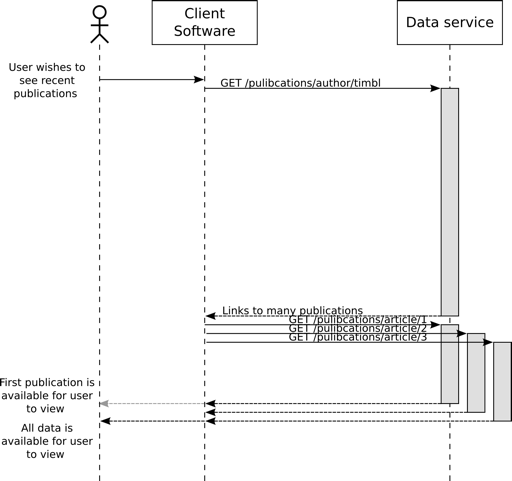
\includegraphics{images/rest_timeline_1.png}
\caption{\textbf{Sequence diagram showing the aggregation of low-level
REST resources by an intermediary.} A client fetches an author's
publication list and then their first three articles. This sequence
represents the most commonly used technique in which the client does not
react to the response until it is complete. In this example the second
wave of requests cannot be made until the original response is complete,
at which time they are issued in quick succession.
\label{rest_timeline_1}}
\end{figure}

\begin{figure}[htbp]
\centering
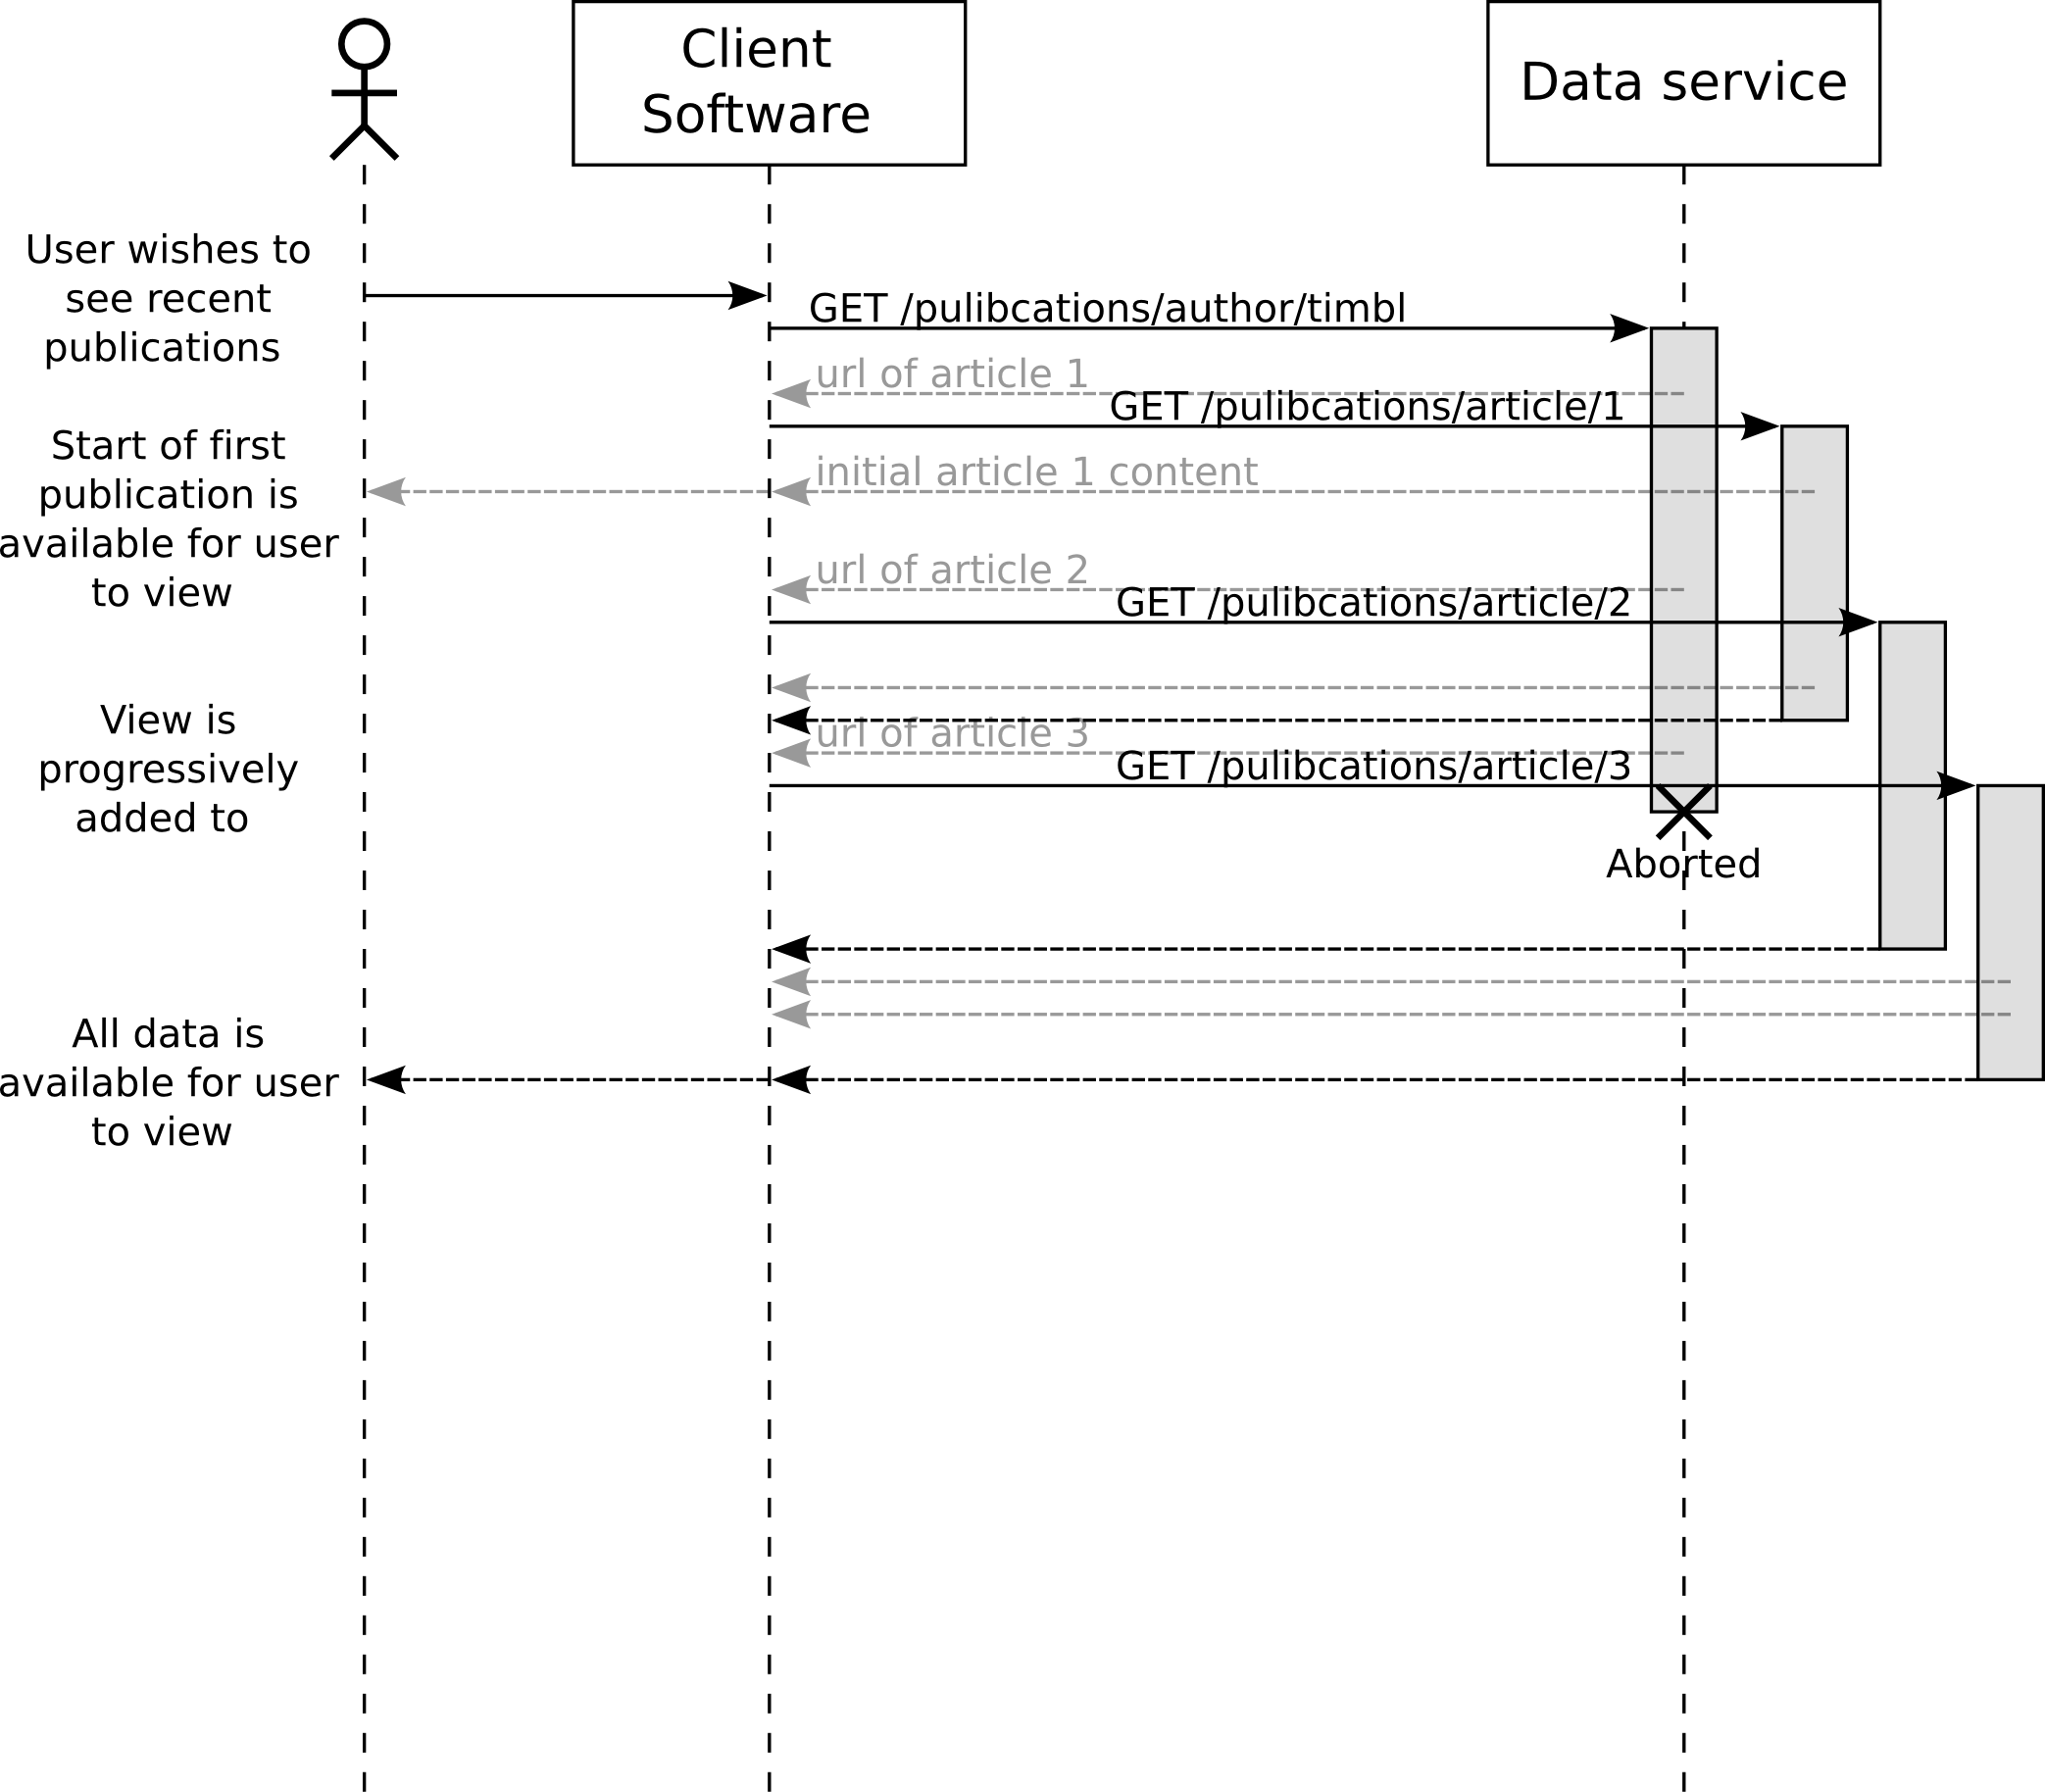
\includegraphics{images/rest_timeline_2.png}
\caption{\textbf{Revised aggregation sequence for a client capable of
progressively interpreting the resources.} Because arrows in UML
sequence diagrams draw returned values as a one-off happening rather
than a continuous process, I have introduced a lighter arrow notation
representing fragments of an incremental response. Each request for an
individual publication is made as soon as the its URL can be extracted
from the publications list and once all required data has been read from
the original response it is aborted rather than continuing to download
unnecessary data. \label{rest_timeline_2}}
\end{figure}

Figures \ref{rest_timeline_1} and \ref{rest_timeline_2} comparatively
illustrate how a progressive client may, without adjustments to the
server, be used to produce an aggregated resource sooner. This results
in a moderate improvement in the time taken to show the complete
aggregation but a dramatic improvement in the time to show the first
content. The ability to present the first content as early as possible
is a desirable trait for system usability because it allows the user to
start reading earlier and a progressively rendered display in itself
increases the human perception of speed (Geelhoed et al. 1995). Note
also how the cadence of requests is more steady in Figure
\ref{rest_timeline_2} with four connections opened at roughly equal
intervals rather than a single request followed by a rapid burst of
three. Both clients and servers routinely limit the number of
simultaneous connections per peer so avoiding bursts is further to our
advantage. \hyperref[appendix_http_limits]{Appendix i} lists some actual
limits.

Nodes in an n-tier architecture defy categorisation as `client' or
`server' in a way which is appropriate from all frames of reference. A
node might be labeled as the `server' from the layer below and `client'
from the layer above. Although the ``client software'' labels in the
figures \ref{rest_timeline_1} and \ref{rest_timeline_2} hint at
something running directly on a user's own device, the same benefits
apply if this layer is running remotely. If this layer were generating a
web page on the server-side to be displayed by the client's browser, the
same perceptual speed improvements apply because of http chunked
encoding (Stefanov 2009). If this layer were a remote aggregation
service, starting to write out the aggregated response early provides
much the same benefits for a client able to interpret it progressively
and, even if it is not, the overall delivery remains faster.

\subsection{Stepping outside the big-small tradeoff}

Where a domain model is requestable via REST and contains data in a
series with continuous ranges I have often noticed a tradeoff in client
design with regards to how much should be requested with each call.
Because at any time it shows only a small window into a much larger
model, the social networking site Twitter might be a good example. The
Twitter interface designers adopted a popular interface pattern,
Infinite Scrolling (Ahuvia 2013). Starting from an initial page showing
some finite number of tweets, once the user scrolls and reaches the end
of the list the next batch is automatically requested. When loaded, this
new batch is converted to HTML and added to the bottom of the page.
Applied repeatedly the illusion of an infinitely long page in
maintained, albeit punctuated with pauses whenever new content is
loaded. For the programmers working on this presentation layer there is
a tradeoff between sporadically requesting many tweets, yielding long,
infrequent delays and frequently requesting a few, giving an interface
which stutters momentarily but often.

I propose that progressive loading could render this tradeoff
unnecessary by simultaneously delivering the best of both strategies. In
the Twitter example this could be achieved by making large requests but
instead of deferring all rendering until the request completes, add the
individual tweets to the page as they are incrementally parsed out of
the ongoing response. With a streaming transport, the time taken to
receive the first tweet should not vary depending on the total number
that are also being sent so there is no relationship between the size of
the request made and the time required to first update the interface.

\subsection{Staying fast on a fallible network}

REST operates over networks whose reliability varies widely. On
unreliable networks connections are abruptly dropped and in my opinion
existing http clients handle unexpected terminations suboptimally.
Consider the everyday situation of a person using a smartphone browser
to check their email. Mobile data coverage is often weak outside of
major cities (Gill 2013) so while travelling the signal will be lost and
reestablished many times. The web developer's standard toolkit is
structured in a way that encourages early terminated connections to be
considered as wholly unsuccessful rather than as partially successful.
For example, the popular AJAX library jQuery automatically parses JSON
or XML responses before passing back to the application but given an
early disconnection there is no attempt to hand over the partial
response. To the programmer who knows where to look the partial
responses are extractable as raw text but handling them involves writing
a special case and is difficult because standard parsers are not
amenable to incomplete markup. Because of this difficulty I can only
find examples of partial messages being dropped without inspection. For
the user checking her email, even if 90\% of her inbox had been
retrieved before her phone signal was lost, the web application will
behave as if it received none and show her nothing. Later, when the
network is available again the inbox will be downloaded from scratch,
including the 90\% which has already been successfully delivered. I see
much potential for improvement here.

I propose moving away from this polarised view of
successful/unsuccessful requests to one in which identifiable parts of a
message are recognised as interesting in themselves, regardless of what
follows, and these parts are handed back to the application as streaming
occurs. This follows naturally from a conceptualisation of the http
response as a progressive stream of many small parts; as each part
arrives it should be possible to use it without knowing if the next will
be delivered successfully. Should an early disconnection occur, the
content delivered up to that point will have already been handled so no
special case is required to salvage it. In most cases the only recovery
necessary will be to make a new request for just the part that was
missed. This approach is not incompatible with a problem domain where
the usefulness of an earlier part is dependent on the correct delivery
of the whole providing optimistic locking is used. In this case earlier
parts may be used immediately but their effect rolled back should a
notification of failure be received.

\subsection{Agile methodologies, frequent deployments, and compatibility
today with versions tomorrow}

In most respects a SOA architecture fits well with the fast release
cycle encouraged by Agile methodologies. Because in SOA we may consider
that all data is local rather than global and that the components are
loosely coupled and autonomous, frequent releases of any particular
sub-system shouldn't pose a problem to the correct operation of the
whole. In allowing a design to emerge organically it should be possible
for the structure of resource formats to be realised slowly and
iteratively while a greater understanding of the problem is gained.
Unfortunately in practice the ability to change often is hampered by
tools which encourage programming against rigidly specified formats.
When a data consumer is allowed to be tightly coupled to a data format
it will resist changes to the programs which produce data in that
format. Working in enterprise I have often seen the release of dozens of
components cancelled because of a single unit that failed to meet
acceptance criteria. By insisting on exact data formats, subsystems
become tightly coupled and the perfect environment is created for
contagion whereby the updating of any single unit may only be done as
part of the updating of the whole.

An effective response to this problem would be to integrate into a REST
clients the ability to use a response whilst being only loosely coupled
to the overall \emph{shape} of the message.

\subsection{Deliverables}

To avoid feature creep I am paring down the software deliverables to the
smallest work which can we said to realise my thesis, the guiding
principle being that it is preferable to produce a little well than more
badly. Amongst commentators on start-up companies this is known as a
\emph{zoom-in pivot} (Reis 2011 p172) and the work it produces should be
the \emph{Minimum Viable Product} or MVP (Reis 2011 p106-110). With a
focus on quality I could not deliver a full stack so I am obliged to
implement only solutions which interoperate with existing deployments.
This is advantageous; to somebody looking to improve their system small
enhancements are more inviting than wholesale change.

To reify the vision above a streaming client is the MVP. Although an
explicitly streaming server would improve the situation further, because
all network transmissions may be viewed though a streaming lens it is
not required to start taking advantage of progressive REST. In the
interest of creating something new, whilst http servers capable of
streaming are quite common even if they are not always programmed as
such, I have been unable to find any example of a streaming-receptive
REST client.

\subsection{Criteria for success}

In evaluating this project we may say it has been a success if
non-trivial improvements in speed can be made without a corresponding
increase in the difficulty of programming the client. This improvement
may be in terms of the absolute total time required to complete a
representative task or in a user's perception of the application
responsiveness while performing the task. Because applications in the
target domain are much more I/O-bound than CPU-bound, optimisation in
terms of the execution time of a algorithms will be de-emphasised unless
especially egregious. Additionally, I shall be considering how the
semantics of a message are expanded as a system's design emerges and
commenting on the value of loose coupling between data formats and the
programs which act on them in avoiding disruption given unanticipated
format changes.

\section{Background}

\begin{figure}[htbp]
\centering
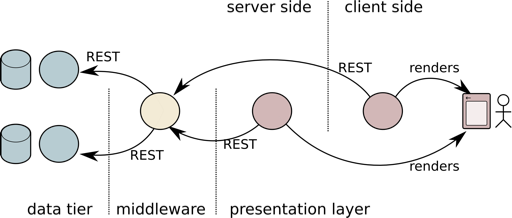
\includegraphics{images/architecture.png}
\caption{\textbf{Labelling nodes in an n-tier architecture}. Regardless
of where a node is located, REST may be used as the means of
communication. By focusing on REST clients, nodes in the middleware and
presentation layer fall in our scope. Although network topology is often
split about client and server side, for our purposes categorisation as
data, middleware, and presentation is the more meaningful distinction.
According to this split the client-side presentation layer and
server-side presentation layer serve the same purpose, generating
mark-up based on aggregated data prepared by the middle tier
\label{architecture}}
\end{figure}

\subsection{The web as an application platform}

Application design has historically charted an undulating path pulled by
competing approaches of thick and thin clients. Having evolved from a
document viewing system to the preferred application platform for all
but the most specialised interfaces, the web perpetuates this narrative
by resisting categorisation as either mode.

While the trend is generally for more client scripting and for many
sites a Javascript runtime is now requisite, there are also
counter-trends. In 2012 twitter reduced load times to one fifth of their
previous design by moving much of their rendering back to the
server-side, commenting that ``The future is coming and it looks just
like the past'' (Lea 2012). Under this architecture short, fast-loading
pages are generated on the server-side but Javascript also provides
progressive enhancements. Although it does not generate pages anew, the
Javascript must know how to create most of the interface elements so one
weakness of this architecture is that much of the presentation layer
logic must be expressed twice.

Despite client devices taking on responsibilities which would previously
have been performed on a server, there is a limit to how much of the
stack may safely be offloaded in this direction. The client-side
ultimately falls under the control of the user so no important business
decisions should be taken here. A banking site should not allow loan
approval to take place in the browser because for the knowledgeable user
any decision would be possible. Separated from data stores by the public
internet, the client is also a poor place to perform data aggregation or
examine large data sets. For non-trivial applications these restrictions
encourage a middle tier to execute business logic and produce aggregate
data.

While REST may not be the only communications technology employed by an
application architecture, for this project we should examine where REST
clients libraries may fit into the picture. REST is used by the
presentation layer to pull data from middleware regardless of where the
presentation resides. Likewise, rather than connect to databases
directly, for portability middlewares often communicate with a thin REST
layer which wraps data stores. This suggests three uses:

\begin{itemize}
\itemsep1pt\parskip0pt\parsep0pt
\item
  From web browser to middleware
\item
  From server-side presentation layer to middleware
\item
  From middleware to nodes in a data tier
\end{itemize}

Fortunately, each of these contexts requires a similar performance
profile. The work done is computationally light and answering a request
involves more time waiting than processing. The node is essentially
acting as a data router serving messages containing a small subset of
the data from a larger model. As a part of an interactive system low
latency is important whereas throughput can be increased relatively
cheaply by adding more hardware, especially in a cloud hosted
environment. As demand for the system increases the total work required
grows but the complexity in responding to any one of the requests
remains constant. Although serving any particular request might be done
in series, the workload as a whole is embarrassingly parallelisable.

\subsection{Node.js}

Node.js is a general purpose tool for executing Javascript outside of a
browser. It has the aim of low-latency I/O and is used mostly for server
applications and command line tools. It is difficult to judge to what
degree Javascript is a distraction from Node's principled design and to
what degree the language defines the platform.

For most imperative languages the thread is the basic unit of
concurrency, whereas Node presents the programmer with a single-threaded
abstraction. Threads are an effective means to share parallel
computation over multiple cores but are less well suited to scheduling
concurrent tasks which are mostly I/O dependent. Programming threads
safely with shared access to mutable objects requires great care and
experience, otherwise the programmer is liable to create race
conditions. Consider for example a Java http aggregator; because we wish
to fetch in parallel each http request is assigned to a thread. These
`requester' tasks are computationally simple: make a request, wait for a
complete response, and then participate in a Barrier while the other
requesters complete. Each thread consumes considerable resources but
during its multi-second lifespan requires only a fraction of a
millisecond on the CPU. It is unlikely any two requests return closely
enough in time that the threads will process in series rather than
parallel, loosing thread's natural strengths for utilising multiple
cores. Even if they do, the actual CPU time required in making an http
request is so short that any concurrent processing is a pyrrhic victory.

\begin{figure}[htbp]
\centering

\includegraphics{images/placeholder.png}
\caption{\textbf{Single-threaded vs multi-threaded scheduling for an
http aggregator}}
\end{figure}

Node builds on the model of event-based, asynchronous i/o that was
established by web browser Javascript execution. Although Javascript in
a browser may be performing multiple tasks simultaneously, for example
requesting several resources from the server side, it does so from
within a single-threaded virtual machine. Node facilitates concurrency
by managing an event loop of queued tasks and providing exclusively
non-blocking I/O. Unlike Erlang, Node does not swap tasks out
preemptively, it always waits for a task to complete before moving onto
the next. This means that each task must complete quickly to avoid
holding up others. \emph{Prima facie} this might seem like an onerous
requirement to put on the programmer but in practice with only
non-blocking I/O available each task naturally exits quickly without any
special effort. Accidental non-terminating loops or heavy
number-crunching aside, with no reason for a task to wait it is
difficult to write a node program in which the tasks do not complete
quickly.

Each task in node is simply a Javascript function. Node is able to swap
its single Javascript thread between these tasks efficiently while
providing the programmer with an intuitive interface because of
closures. Utilising closures, the responsibility of maintaining state
between issuing an asynchronous call and receiving the callback is
removed from the programmer by folding the storage invisibly into the
language. This implicit data store requires no syntax and feels so
natural and inevitable that it is often not obvious that the
responsibility exists at all.

Consider the example below. The code schedules three tasks, each of
which are very short and exit quickly allowing Node to finely interlace
them between other concurrent concerns. The \texttt{on} method is used
to attach functions as listeners to streams. However sophisticated and
performant this style of programming, to the developer it is hardly any
more difficult an expression than if I/O were used. It is certainly
harder to make mistakes programming in this way than managing
synchronised access to mutable objects that are shared between threads.

\begin{Shaded}
\begin{Highlighting}[]
\KeywordTok{function} \FunctionTok{printResourceToConsole}\NormalTok{(url) \{}

   \OtherTok{http}\NormalTok{.}\FunctionTok{get}\NormalTok{(url)}
      \NormalTok{.}\FunctionTok{on}\NormalTok{(}\StringTok{'response'}\NormalTok{, }\KeywordTok{function}\NormalTok{(response)\{}
      
         \CommentTok{// This function will be called when the response starts.}
         \CommentTok{// It logs to the console, adds a listener and quickly }
         \CommentTok{// exits.}
         
         \CommentTok{// Because it is captured by a closure we are able to }
         \CommentTok{// reference the url parameter after the scope that }
         \CommentTok{// declared it has finished.            }
         \OtherTok{console}\NormalTok{.}\FunctionTok{log}\NormalTok{(}\StringTok{"The response has started for "}\NormalTok{, url);}
      
         \OtherTok{response}\NormalTok{.}\FunctionTok{on}\NormalTok{(}\StringTok{'data'}\NormalTok{, }\KeywordTok{function}\NormalTok{(chunk) \{      }
            \CommentTok{// This function is called each time some data is}
            \CommentTok{// received from the http request. The task writes}
            \CommentTok{// the response to the console and quickly exits.}
            \OtherTok{console}\NormalTok{.}\FunctionTok{log}\NormalTok{(}\StringTok{'Got some response '}\NormalTok{, chunk);}
                   
         \NormalTok{\}).}\FunctionTok{on}\NormalTok{(}\StringTok{'end'}\NormalTok{, }\KeywordTok{function}\NormalTok{()\{}
            \OtherTok{console}\NormalTok{.}\FunctionTok{log}\NormalTok{(}\StringTok{'The response is complete'}\NormalTok{);}
         \NormalTok{\})}
         
      \NormalTok{\}).}\FunctionTok{on}\NormalTok{(}\StringTok{"error"}\NormalTok{, }\KeywordTok{function}\NormalTok{(e)\{}
         
         \OtherTok{console}\NormalTok{.}\FunctionTok{log}\NormalTok{(}\StringTok{"There was an error: "} \NormalTok{+ }\OtherTok{e}\NormalTok{.}\FunctionTok{message}\NormalTok{);}
      \NormalTok{\});      }
   \OtherTok{console}\NormalTok{.}\FunctionTok{log}\NormalTok{(}\StringTok{"The request has been made"}\NormalTok{);}
\NormalTok{\}   }
\end{Highlighting}
\end{Shaded}

\begin{quote}
``Node Stream API, which is the core I/O abstraction in Node.js (which
is a tool for I/O) is essentially an abstract in/out interface that can
handle any protocol/stream that also happens to be written in
JavaScript.'' (Ogden 2012)
\end{quote}

In Node I/O is performed using a unified data streaming interface
regardless of the source. The streams fit comfortably with the wider
event-driven model by implementing Node's EventEmitter interface, a
generic Observer pattern API. Although the abstraction provided by
streams is quite a thin layer on top of the host system's socket, it
forms a powerful and intuitive interface. For many tasks it is
preferable to program in a `plumbing' style by joining one stream's
output to another's input. In the example below a resource from the
internet is written to the local filesystem.

\begin{Shaded}
\begin{Highlighting}[]
\OtherTok{http}\NormalTok{.}\FunctionTok{get}\NormalTok{(url)}
   \NormalTok{.}\FunctionTok{on}\NormalTok{(}\StringTok{'response'}\NormalTok{, }\KeywordTok{function}\NormalTok{(response)\{}
      \OtherTok{response}\NormalTok{.}\FunctionTok{pipe}\NormalTok{(}\OtherTok{fs}\NormalTok{.}\FunctionTok{createWriteStream}\NormalTok{(pathToFile));}
   \NormalTok{\});}
\end{Highlighting}
\end{Shaded}

Following Node's lead, traditionally thread-based environments are
beginning to embrace asynchronous, single-threaded servers. The Netty
project can be though of as roughly the Java equivalent of Node.

\subsection{Json and XML data transfer formats}

Both XML and JSON are text based, tree shaped data formats with human
and machine readability. One of the design goals of XML was to simplify
SGML to the point that a graduate student could implement a full parser
in a week (Eberhart and Fischer 2002 p287). Continuing this arc of
simpler data formats, JSON ``The fat-free alternative to XML (Douglas
2009)'' isolates Javascript's syntax for literal values into a
stand-alone serialisation language. For the graduate tackling JSON
parsing the task is simpler still, being expressible as fifteen context
free grammars.

Whereas XML's design can be traced to document formats, JSON's lineage
is in a programming language. From these roots isn't surprising that
JSON maps more directly to the metamodel that most programmers think in.
XML parsers produce Elements, Text, Attributes, ProcessingInstruction
which require extra translation before they are convenient to use inside
a programming language. Because JSON already closely resembles how a
programmer would construct a runtime model of their data, fewer steps
are required before using the deserialised form. The JSON nodes:
\emph{strings}, \emph{numbers}, \emph{objects} and \emph{arrays} will in
many cases map directly onto language types and, for loosely typed
languages at least, the parser output bears enough similarity to domain
model objects that it may be used directly without any further
transformation.

\begin{Shaded}
\begin{Highlighting}[]
\NormalTok{\{}
   \DataTypeTok{people}\NormalTok{: [}
      \NormalTok{\{}\DataTypeTok{name}\NormalTok{: }\StringTok{'James'}\NormalTok{, }\DataTypeTok{town}\NormalTok{:}\StringTok{'London'}\NormalTok{\},}
      \NormalTok{\{}\DataTypeTok{name}\NormalTok{: }\StringTok{'Thomas'}\NormalTok{, }\DataTypeTok{town}\NormalTok{:}\StringTok{'Bristol'}\NormalTok{\}}
      \NormalTok{\{}\DataTypeTok{town}\NormalTok{:}\StringTok{'Cambridge'}\NormalTok{, }\DataTypeTok{name}\NormalTok{: }\StringTok{'Sally'}\NormalTok{\}}
   \NormalTok{]}
\NormalTok{\}}
\end{Highlighting}
\end{Shaded}

Both JSON and XML are used to serialise to and from orderless constructs
but but while serialised to text, an ordered list of characters, the
nodes are inevitably encountered according to some serialisation order.
There is no rule forbidding serialisation to JSON or XML attributes in
an order-significant way but in general the order is considered to not
be significant in the serialised format's model. In the example above,
the people objects would probably have been written out to represent
either a class with two public properties or a hash map. On receiving
this data the text would be demarshalled into similar structures and
that the data found an ordered expression during transport would be
quickly forgotten. However, when viewing a document through a streaming
and interpreting documents while still incomplete this detail cannot be
ignored as a concern relating only to the accidents of transfer. If
nodes were interpreted based on their first field in the example above
Walter would find a different handling than the other two. Because the
serialisation will contain items which are written to follow an
indeterminate order it will be important to ensure that, despite the
streaming, the REST client does not encourage programming in a way that
depends on the order that these fields are received.

\subsection{Common patterns for connecting to REST services}

For languages such as Javascript or Clojure with a loosely-typed
representation of objects as generic key-value pairs, when a JSON REST
resource is received, the output from the parser resembles the normal
object types closely enough that it is acceptable to use it directly
throughout the program. For XML this is not the case and some marshaling
is required. In more strongly typed OO languages such as Java or C\#,
JSON's relatively freeform, classless objects are less convenient. For
the example JSON from \hyperref[jsonxml2]{the previous section} to be
smoothly consumed, instantiating instances of a domain model Person
class with methods such as \texttt{getName()} and \texttt{getTown()}
would be preferable, representing the remote resource's objects no
differently than if they had originated locally. Automatic marshaling
generalises this process by providing a two-way mapping between the
domain model and its serialisation, either completely automatically or
based on a declarative specification. It is common in strongly typed
languages for REST client libraries to automatically demarshal as part
of receiving a fetched rest response. From the programmer's vantage it
is as if the domain objects themselves had been fetched. Adding an
additional layer, another common design pattern intended to give a
degree of isolation between remote resources and the local domain model
is to demarshal automatically only so far as \emph{Data Transfer
Objects} (DTOs). DTOs are instances of classes which implement no logic
other than storage, and from these DTOs the domain model objects may be
programmatically instantiated. DTOs are more necessary when using XML.
For reading JSON resources we might say that the JSON objects \emph{are}
the DTOs.

The degree of marshaling that is used generally changes only the types
of the entities that the REST client library hands over to the
application developer without affecting the overall structure of the
message. Regardless of the exact types given, having received the
response model the developer will usually start by addressing the
pertinent parts of the response by drilling down into the structures
using assessor operators from the programming language itself.

\begin{Shaded}
\begin{Highlighting}[]
\CommentTok{// Java example - programmatic approach to domain model interrogation }

\CommentTok{// The methods used to drill down to desired components }
\CommentTok{// are all getters: getPeople, getName, and getTown.}
 
\DataTypeTok{void} \FunctionTok{handleResponse}\NormalTok{( RestResponse response ) \{}

   \KeywordTok{for}\NormalTok{( Person p : response.}\FunctionTok{getPeople}\NormalTok{() ) \{}
      \FunctionTok{addPersonToDb}\NormalTok{( p.}\FunctionTok{getName}\NormalTok{(), p.}\FunctionTok{getTown}\NormalTok{() );}
   \NormalTok{\}   }
\NormalTok{\}}
\end{Highlighting}
\end{Shaded}

\begin{Shaded}
\begin{Highlighting}[]
\CommentTok{// equivalent Javascript - the programming follows the same basic}
\CommentTok{// process. This time using Javascript's dot operator.}

\KeywordTok{function} \FunctionTok{handleResponse}\NormalTok{( response )\{}

   \OtherTok{response}\NormalTok{.}\OtherTok{people}\NormalTok{.}\FunctionTok{forEach}\NormalTok{( }\KeywordTok{function}\NormalTok{( person )\{}
      \FunctionTok{addPersonToDb}\NormalTok{( }\OtherTok{p}\NormalTok{.}\FunctionTok{name}\NormalTok{, }\OtherTok{p}\NormalTok{.}\FunctionTok{town} \NormalTok{);}
   \NormalTok{\});}
\NormalTok{\}}
\end{Highlighting}
\end{Shaded}

One weakness in this means of drilling down is that the code making the
inspection is quite tightly coupled to the precise structure of the
thing that it is inspecting. Taking the above example, if the resource
being fetched were later refactored such that the town concept were
refactored into a fuller address with a town-county-country tuple, the
code addressing the structure would also have to change just to continue
to do the same thing. Although this kind of drill-down programming is
commonly practiced and not generally recognised as a code smell,
requiring knock-on changes when an unrelated system is refactored seems
to me as undesirable here as it would be anywhere else.

In \emph{the Red Queen's race} it took ``all the running you can do, to
keep in the same place''. Ideally as a programmer I'd like to expend
effort to make my code to do something new, or to perform something that
it already did better, not so that it keeps the same. Following an
object oriented encapsulation of data such that a caller does not have
to concern themselves with the data structures behind an interface, the
internal implementation may be changed without disruptions to the rest
of the code base. However when the structure of the inter-object
composition is revised, isolation from the changes is less often
recognised as a desirable trait. A method of programming which truly
embraced extreme programming would allow structural refactoring to occur
without disparate, parts having to be modified in parallel.

Extraneous changes also dilute a VCS changelog, making it less easily to
later follow a narrative of code changes which are intrinsic to the
difference in logic expressed by the program, and therefore harder to
later understand the thinking behind the change and the reason for the
change.

\subsection{JsonPath and XPath selector languages}

\label{jsonpathxpath}

The problem of drilling down to pertinent fragments of a message without
tightly coupling to the format could be somewhat solved if instead of
programmatically descending step-by-step, a language were used which
allows the right amount of specificity regarding which parts to select.
For markup languages there are associated query languages whose coupling
is loose enough that not every node that is descended through must be
specified. The best known is XPATH but there is also JSONPath, a JSON
equivalent (Goessner 2007).

As far as possible the JSONPath language follows the javascript to
descend into the same sub-tree.

\begin{Shaded}
\begin{Highlighting}[]
\CommentTok{// in Javascript we can get the town of the second person as:}
\KeywordTok{let} \NormalTok{town = }\OtherTok{subject}\NormalTok{.}\FunctionTok{people}\NormalTok{[}\DecValTok{2}\NormalTok{].}\FunctionTok{town}

\CommentTok{// the equivalent JSONPath expression is identical:}
\KeywordTok{let} \NormalTok{townSelector = }\StringTok{"people[2].town"}

\CommentTok{// We would be wise not to write overly-specific selectors.}
\CommentTok{// JSONPath also provides an ancestor relationship not found in Javascript:}
\KeywordTok{let} \NormalTok{betterTownSelector = }\StringTok{"people[2]..town"}
\end{Highlighting}
\end{Shaded}

Consider the resource below:

\begin{Shaded}
\begin{Highlighting}[]
\NormalTok{\{}
   \DataTypeTok{people}\NormalTok{: [}
      \NormalTok{\{}\DataTypeTok{name}\NormalTok{: }\StringTok{'John'}\NormalTok{, }\DataTypeTok{town}\NormalTok{:}\StringTok{'Oxford'}\NormalTok{\},}
      \NormalTok{\{}\DataTypeTok{name}\NormalTok{: }\StringTok{'Jack'}\NormalTok{, }\DataTypeTok{town}\NormalTok{:}\StringTok{'Bristol'}\NormalTok{\}}
      \NormalTok{\{}\DataTypeTok{town}\NormalTok{:}\StringTok{'Cambridge'}\NormalTok{, }\DataTypeTok{name}\NormalTok{: }\StringTok{'Walter'}\NormalTok{\}}
   \NormalTok{]}
\NormalTok{\}}
\end{Highlighting}
\end{Shaded}

The JSONPath \texttt{people.*..town} against the above JSON format would
continue to select correctly after a refactor to the JSON below:

\begin{Shaded}
\begin{Highlighting}[]
\NormalTok{\{}
   \DataTypeTok{people}\NormalTok{: [}
      \NormalTok{\{  }\DataTypeTok{name}\NormalTok{: }\StringTok{'John'}\NormalTok{, }
         \DataTypeTok{address}\NormalTok{:\{}\DataTypeTok{town}\NormalTok{:}\StringTok{'Oxford'}\NormalTok{, }\DataTypeTok{county}\NormalTok{:}\StringTok{'Oxon'}\NormalTok{, }\DataTypeTok{country}\NormalTok{:}\StringTok{'uk'}\NormalTok{\}}
      \NormalTok{\},}
      \NormalTok{\{  }\DataTypeTok{name}\NormalTok{: }\StringTok{'Jack'}\NormalTok{,}
         \DataTypeTok{address}\NormalTok{:\{}\DataTypeTok{town}\NormalTok{:}\StringTok{'Bristol'}\NormalTok{, }\DataTypeTok{county}\NormalTok{:}\StringTok{'Bristol'}\NormalTok{, }\DataTypeTok{country}\NormalTok{:}\StringTok{'uk'}\NormalTok{\}}
      \NormalTok{\}}
      \NormalTok{\{  }\DataTypeTok{address}\NormalTok{:\{}
            \DataTypeTok{town}\NormalTok{:}\StringTok{'Cambridge'}\NormalTok{, }\DataTypeTok{county}\NormalTok{:}\StringTok{'Cambridgeshire'}\NormalTok{, }
            \DataTypeTok{country}\NormalTok{:}\StringTok{'uk'}
         \NormalTok{\},}
         \DataTypeTok{name}\NormalTok{: }\StringTok{'Walter'}
      \NormalTok{\}}
   \NormalTok{]}
\NormalTok{\}}
\end{Highlighting}
\end{Shaded}

Maintaining compatibility with unanticipated format revisions through
selector languages is easier with JSON than XML. The XML metamodel
contains overlapping representations of equivalent entities which a
refactored format is liable to switch between. Each XML element has two
distinct lists of child nodes, attribute children and node list
children; from one perspective attributes are child nodes of their
parent element but they can alternatively be considered as data stored
in the element. Because of this classification ambiguity an XML document
doesn't form a single, correct n-way tree. Because of the difference in
expressivity between attributes which may only be strings and child
nodes which allow recursive structure, this is a common refactor when a
more detailed mapping is required and a scalar value is upgraded to be
compound. XPath selectors written in the most natural way do not track
this change.

\begin{Shaded}
\begin{Highlighting}[]
\KeywordTok{<people>}
   \KeywordTok{<person}\OtherTok{ name=}\StringTok{"John"}\OtherTok{ town=}\StringTok{"Oxford"}\KeywordTok{></person>}
\KeywordTok{</people>}
\end{Highlighting}
\end{Shaded}

The XPath \texttt{//person@town} matches the XML above but because of
the refactor from attribute to child element fails to match the revised
version below.

\begin{Shaded}
\begin{Highlighting}[]
\KeywordTok{<people>}
   \KeywordTok{<person>}
      \KeywordTok{<name>}
         \NormalTok{John}
      \KeywordTok{</name>}
      \KeywordTok{<address>}
         \KeywordTok{<town>}\NormalTok{Oxford}\KeywordTok{</town>} \KeywordTok{<county>}\NormalTok{Oxon}\KeywordTok{</county>}
      \KeywordTok{</address>}
   \KeywordTok{</person>}
\KeywordTok{</people>}
\end{Highlighting}
\end{Shaded}

Reflecting its dual purpose for marking up for documents or data, XML
also invites ambiguous interpretation of the whitespace between tags.
Whitespace is usually meaningful for documents but ignorable for data.
Strictly, whitespace text nodes are a part of the document but in
practice many tree walkers discard them as insignificant. In the XML
above the \texttt{\textless{}person\textgreater{}} element may be
enumerated as either the first or second child of
\texttt{\textless{}people\textgreater{}} depending on whether the
whitespace before it is considered. Likewise, the text inside
\texttt{\textless{}name\textgreater{}} might be \texttt{'John'} or
\texttt{'(newline)(tab)(tab)John'}. Inherited from JSON's programming
language ancestry, the space between tokens is never significant.

Programming against a changing service is always going to be a moving
target, but it is easier to miss with XPATH than with JSON. In JSON each
nodes has only one, unambiguous set of children so the metamodel does
not present the format author with a selection from logical equivalents
that are addressed through different mechanisms. If a scalar value is
updated to a compound only the node itself changes, the addressing of
the node is unaffected.

Generally in descriptive hierarchical data there is a trend for
ancestorship to denote the same relationship between concepts regardless
of the number of intermediate generations. In the example above,
\texttt{town} transitioned from child to grandchild of \texttt{person}
without disturbing the implicit `lives in' relationship. In JSONPath the
\texttt{..} operator provides matching through zero or more generations,
unperturbed when extra levels are added. Of course, this trend will not
hold for every conceivable way of building message semantics because it
is possible that an intermediate node on the path from ancestor to
descendant will change the nature of the expressed relationship. A
slightly contrived example might be if we expanded our model to contain
fuzzy knowledge:

\begin{Shaded}
\begin{Highlighting}[]
\KeywordTok{<people>}
   \KeywordTok{<person>}
      \KeywordTok{<name>}
         \KeywordTok{<isProbably>}\NormalTok{Bob}\KeywordTok{</isProbably>}
      \KeywordTok{</name>}
   \KeywordTok{</person>}
\KeywordTok{</people>}
\end{Highlighting}
\end{Shaded}

Considering the general case, it will not be possible to track all
possible service refactors safely. By necessity a resource consumer
should limit their ambitions to tracking ontology additions which do not
change the meaning of the existing concepts. In practice integration
testing against the beta version of a service will be necessary to be
pre-warned of upcoming, incompatible changes. If an incompatibility is
found the ability to then create an expression which is compatible with
with a present and known future version remains a valuable tool because
it decouples service consumer and provider update schedules, removing
the need for the client to march perfectly in sync with the service.

\subsection{Browser XML HTTP Request (XHR)}

Making http requests from Javascript, commonly termed AJAX, was so
significant in establishing the modern web architecture that it is
sometimes used synonymously with Javascript-rich web applications.
Although AJAX is an acronym for \textbf{A}synchronous
\textbf{J}avascript (\textbf{a}nd) \textbf{X}ML, this reflects the early
millennial enthusiasm for XML as the one true data format and in
practice any textual format may be transferred. Today JSON is generally
preferred, especially for delivery to client-side web applications.
During the `browser war' years web browsers competed by adding
non-standard features; Internet Explorer made AJAX possible in 2000 by
exposing Microsoft's Active X \emph{Xml Http Request} (XHR) class to the
Javascript sandbox. This was widely copied and near equivalents were
added to all major browsers. In 2006 the interface was eventually
formalised by the W3C (van Kesteren and Jackson 2006). XHR's slow
progresss to standardisation reflected a period of general stagnation
for web standards. HTML4 reached Recommendation status in 2001 but
having subsequently found several evolutionary dead ends such as XHTML,
there would be no major updates until HTML5 started to gather pace some
ten years later.

Despite a reputation for being poorly standardised, as a language
Javascript enjoys consistent implementation. More accurately we would
say that browser APIs exposed to Javascript lack compatibility. Given
this backdrop of vendor extensions and lagging standardisation,
abstraction layers predictably rose in popularity. Various abstractions
competed primarily on developer ergonomics with the popular jQuery and
Prototype.js libraries promoting themselves as \emph{``do more, write
less''} and \emph{``elegant APIs around the clumsy interfaces of
Ajax''}. Written against the unadorned browser, Javascript applications
read as a maze of platform-detection and special cases. Once
applications were built using Javascript abstractions over the
underlying browser differences, they could be written purposefully and
were able to express more complex ideas without becoming
incomprehensible.

JSON is today the main format output by REST end points when requesting
via AJAX. Javascript programmers occupy a privileged position whereby
their serialisation format maps exactly onto the inbuilt types of their
programming language. As such there is never any confusion regarding
which object structure to de-serialise to. Should this advantage seem
insubstantial, contrast with the plethora of confusing and incompatible
representations of JSON that are output by the various Java parsers:
JSON's Object better resembles Java's Map interface than Java Objects,
creating linguistic difficulties, and the confusion between JSON null,
Java null, and Jackson's NullNode\footnote{See
  \url{http://jackson.codehaus.org/1.0.1/javadoc/org/codehaus/jackson/node/NullNode.html}.}
is a common cause of errors. Emboldened by certainty regarding
deserialisation, AJAX libraries directly integrated JSON parsers,
providing a call style for working with remote resources so streamlined
as to require hardly any additional effort.

\begin{Shaded}
\begin{Highlighting}[]
\OtherTok{jQuery}\NormalTok{.}\FunctionTok{ajax}\NormalTok{(}\StringTok{'http://example.com/people.json'}\NormalTok{, }\KeywordTok{function}\NormalTok{( people ) \{}

   \CommentTok{// The parsing of the people json into a javascript object}
   \CommentTok{// feels so natural that it is easy to forget from looking }
   \CommentTok{// at the code that parsing happens at all. }
   
   \FunctionTok{alert}\NormalTok{(}\StringTok{'the first person is called '} \NormalTok{+ people[}\DecValTok{0}\NormalTok{].}\FunctionTok{name}\NormalTok{);}
\NormalTok{\});}
\end{Highlighting}
\end{Shaded}

\subsection{XHRs and streaming}

\label{xhrsandstreaming}

Browser abstraction layers brought an improvement in expressivity to web
application programming but were ultimately limited to supporting the
lowest common denominator of the available browser abilities. At the
time that the call style above was developed the most popular browser
gave no means of access to partial responses. Inevitably, it draws a
conceptualisation of the response as a one-time event with no
accommodation offered for progressively delivered data.

The followup standard, XHR2 is now at Working Draft stage. Given
ambitions to build a streaming REST client, of greatest interest is the
progress event:

\begin{quote}
While the download is progressing, queue a task to fire a progress event
named progress about every 50ms or for every byte received, whichever is
least frequent. (van Kesteren 2012)
\end{quote}

The historic lack of streaming for data fetched using XHR stands
incongruously with the browser as a platform in which almost every other
remote resource is interpreted progressively. Examples include
progressive image formats, html, svg, video, and Javascript itself
(script interpretation starts before the script is fully loaded).

The progress event is supported by the latest version of all major
browsers. However, Internet Explorer only added support recently with
version 10 and there is a significant user base remaining on versions 8
and 9.

\subsection{Browser streaming frameworks}

\label{browserstreamingframeworks}

The web's remit is increasingly widening to encompass scenarios which
would have previously been the domain of native applications. In order
to use live data many current webapps employ frameworks which push soft
real-time events to the client side. In comparison to the XHR2 progress
event, this form of streaming has a different but overlapping purpose.
Whereas XHR2 enables downloads to be viewed as short-lived streams but
does not otherwise disrupt the sequence of http's request-response
model, streaming frameworks facilitate an entirely different sequence,
that of perpetual data. Consider a webmail interface; initially the
user's inbox is downloaded via REST and a streaming download might be
used to speed its display. Regardless of if the response is interpreted
progressively, this inbox download is a standard REST call and shares
little in common with the push events which follow to provide instant
notification as new messages arrive.

\textbf{Push tables} sidestep the browser's absent data streaming
abilities by leaning on a resource that it can stream: progressive html.
From the client a page containing a table is hidden in an off-screen
iframe. This table is served from a a page that never completes, fed by
a connection that never closes. When the server wishes to push a message
to the client it writes a new row in this table which is then noticed by
Javascript monitoring the iframe on the client. More recently,
\textbf{Websockets} is a new standard that builds a standardised
streaming transport on top of http's chunked mode. Websockets requires
browser implementation and cannot be retrofitted to older browsers
through Javascript. Websockets are a promising technology but for the
time being patchy support means it cannot be used without a suitable
fallback.

These frameworks do not interoperate at all with REST. Because the
resources they serve never complete they may not be read by a standard
REST client. Unlike REST they also are not amenable to standard http
mechanics such as caching. A server which writes to an esoteric format
requiring a specific, known, specialised client also feels quite
anti-REST, especially when we consider that the format design reflects
the nature of the transport more so than the resource. This form of
streaming is not, however, entirely alien to a SOA mindset. The data
formats, while not designed primarily for human readability are
nontheless text based and a person may take a peek inside the system's
plumbing simply by observing the traffic at a particular URL. In the
case of push-tables, an actual table of the event's properties may be
viewed from a browser as the messages are streamed.

\subsection{Parsing: SAX and Dom}

From the XML world two standard parser types exist, SAX and DOM, with
DOM by far the more popular. Although the terms originate in XML, both
styles of parsers are also available for JSON. DOM performs a parse as a
single evaluation and returns a single object model representing the
whole of the document. Conversely, SAX parsers are probably better
considered as tokenisers, providing a very low-level event driven
interface following the Observer pattern that notifies the programmer of
each token separately as it is found. From DOM's level of abstraction
the markup syntax is a distant concern whereas for SAX each element's
opening and closing tag is noted so the developer may not put the data's
serialisation aside. SAX has the advantages that it may read a document
progressively and has lower memory requirements because it does not
store the parsed tree. Correspondingly, it it popular for embedded
systems on limited hardware which need to handle documents larger than
the available RAM.

Suppose we have some json representing people and want to extract the
name of the first person. Given a DOM parser this may be written quite
succinctly:

\begin{Shaded}
\begin{Highlighting}[]
\KeywordTok{function} \FunctionTok{nameOfFirstPerson}\NormalTok{( myJsonString ) \{}

   \CommentTok{// All recent browsers provide JSON.parse as standard. }

   \KeywordTok{var} \NormalTok{document = }\OtherTok{JSON}\NormalTok{.}\FunctionTok{parse}\NormalTok{( myJsonString );}
   \KeywordTok{return} \OtherTok{document}\NormalTok{.}\FunctionTok{people}\NormalTok{[}\DecValTok{0}\NormalTok{].}\FunctionTok{name}\NormalTok{; }\CommentTok{// that was easy!}
\NormalTok{\}}
\end{Highlighting}
\end{Shaded}

To contrast, the equivalent below uses SAX, expressed in the most
natural way for the technology.\footnote{For an example closer to the
  real world see
  \url{https://github.com/dscape/clarinet/blob/master/samples/twitter.js}.}

\begin{Shaded}
\begin{Highlighting}[]
\KeywordTok{function} \FunctionTok{nameOfFirstPerson}\NormalTok{( myJsonString, callbackFunction )\{}


   \KeywordTok{var} \NormalTok{clarinet = }\OtherTok{clarinet}\NormalTok{.}\FunctionTok{parser}\NormalTok{(),}
   
       \CommentTok{// With a SAX parser it is the developer's responsibility }
       \CommentTok{// to track where in the document the cursor currently is,}
       \CommentTok{// Several variables are used to maintain this state.        }
       \NormalTok{inPeopleArray = }\KeywordTok{false}\NormalTok{,   }
       \NormalTok{inPersonObject = }\KeywordTok{false}\NormalTok{,}
       \NormalTok{inNameAttribute = }\KeywordTok{false}\NormalTok{,}
       \NormalTok{found = }\KeywordTok{false}\NormalTok{;}
   
   \OtherTok{clarinet}\NormalTok{.}\FunctionTok{onopenarray} \NormalTok{= }\KeywordTok{function}\NormalTok{()\{}
      \CommentTok{// For brevity we'll cheat by assuming there is only one}
      \CommentTok{// array in the document. In practice this would be overly}
      \CommentTok{// brittle.}
      
      \NormalTok{inPeopleArray = }\KeywordTok{true}\NormalTok{; }
   \NormalTok{\};}
   
   \OtherTok{clarinet}\NormalTok{.}\FunctionTok{onclosearray} \NormalTok{= }\KeywordTok{function}\NormalTok{()\{}
      \NormalTok{inPeopleArray = }\KeywordTok{false}\NormalTok{;}
   \NormalTok{\};   }
   
   \OtherTok{clarinet}\NormalTok{.}\FunctionTok{onopenobject} \NormalTok{= }\KeywordTok{function}\NormalTok{()\{}
      \NormalTok{inPersonObject = inPeopleArray; }
   \NormalTok{\};}
   
   \OtherTok{clarinet}\NormalTok{.}\FunctionTok{oncloseobject} \NormalTok{= }\KeywordTok{function}\NormalTok{()\{}
      \NormalTok{inPersonObject = }\KeywordTok{false}\NormalTok{;}
   \NormalTok{\};   }
      
   \OtherTok{clarinet}\NormalTok{.}\FunctionTok{onkey} \NormalTok{= }\KeywordTok{function}\NormalTok{(key)\{}
      \NormalTok{inNameAttribute = ( inPeopleObject && key == }\StringTok{'name'}\NormalTok{);}
   \NormalTok{\};}

   \OtherTok{clarinet}\NormalTok{.}\FunctionTok{onvalue} \NormalTok{= }\KeywordTok{function}\NormalTok{(value)\{}
      \KeywordTok{if}\NormalTok{( !found && inNameAttribute ) \{}
         \CommentTok{// finally!}
         \FunctionTok{callbackFunction}\NormalTok{( value );}
         \NormalTok{found = }\KeywordTok{true}\NormalTok{;}
      \NormalTok{\}}
   \NormalTok{\};      }
   
   \OtherTok{clarinet}\NormalTok{.}\FunctionTok{write}\NormalTok{(myJsonString);   }
\NormalTok{\}}
\end{Highlighting}
\end{Shaded}

The developer pays a high price for progressive parsing, the SAX version
is considerably longer and more difficult to read. SAX's low-level
semantics require a lengthy expression and push the responsibility of
maintaining state regarding the current position in the document and the
nodes that have previously been seen onto the programmer. This
maintenance of state tends to programmed once per usage rather than
assembled as the composition of reusable parts. I find the order of the
code under SAX quite unintuitive; event handlers cover multiple
unrelated cases and each concern spans multiple handlers. This lends to
a style of programming in which separate concerns do not find separate
expression in the code. It is also notable that, unlike DOM, as the
depth of the document being interpreted increases, the length of the
programming required to interpret it also increases, mandating more
state be stored and an increased number of cases be covered per event
handler.

While SAX addresses many of the problems raised in this dissertation, I
find the unfriendly developer ergonomics pose too high a barrier to its
adoption for all but fringe uses.

\section{Design and Reflection:}

Using a combination of techniques from the previous chapter I propose
that it is possible to combine the desirable properties from SAX and DOM
parsers into a REST client library which allows streaming but is also
convenient to program.

By observing the flow of data streams through a SAX parser we can say
that the REST workflow is more efficient if we do not wait until we have
everything before we start using the parts that we do have. However, the
SAX model presents poor developer ergonomics because it is not usually
convenient to think on the level of abstraction that it presents: that
of markup tokens. Using SAX, a programmer may only operate on a
convenient abstraction after inferring it from a lengthy series of
callbacks. In terms of ease of use, DOM is generally preferred because
it provides the resource whole and in a convenient form. My design aims
to duplicate this convenience and combine it with progressive
interpretation by removing one restriction: that the node which is given
is always the document root. From a hierarchical markup such as XML or
JSON, when read in order, the sub-trees are fully known before we fully
know their parent tree. We may select pertinent parts of a document and
deliver them as fully-formed entities as soon as they are known, without
waiting for the remainder of the document to arrive.

By my design, identifying the interesting parts of a document before it
is complete involves turning the established model for drilling-down
inside-out. Under asynchronous I/O the programmer's callback
traditionally receives the whole resource and then, inside the callback,
locates the sub-parts that are required for a particular task. Inverting
this process, I propose extracting the locating logic currently found
inside the callback and using it to decide when the callback should be
used. The callback will receive complete fragments from the response
once they have been selected according to this logic.

I will be implementing using the Javascript language because it has good
support for non-blocking I/O and covers both contexts where this project
will be most useful: in-browser programming and server programming.
Focusing on the MVP, I will only be implementing the parsing of one
mark-up language. Although this technique could be applied to any
text-based, tree-shaped markup, I find that JSON best meets my goals
because it is widely supported, easy to parse, and because it defines a
single n-way tree, is amenable to selectors which span multiple format
versions.

JSONPath is especially applicable to node selection as a document is
read because it specifies only constraints on paths and `contains'
relationships. Because of the top-down serialisation order, on
encountering any node in a serialised JSON stream, I will have already
seen enough of the prior document to know its full path. JSONPath would
not be so amenable if it expressed sibling relationships because there
is no similar guarantee of having seen other nodes on the same level
when any particular node is encountered. A new implementation of the
language is required because the existing JSONPath library is
implemented only as a means to search through already gathered objects
and is too narrow in applicability to be useful in our context.

Not all of the JSONPath language is well suited when we consider we are
selecting specifically inside a REST resource. Given this context it is
likely that we will not be examining a full model but rather a subset
that we requested and was assembled on our behalf according to the
parameters that we supplied. We can expect to be interested in all of
the content so search-style selections such as `books costing less than
X' are less useful than queries which identify nodes because of their
type and position such as `all books in the discount set', or, because
we know we are examining \texttt{/books/discount}, simply `all books'.
In creating a new JSONPath implementation I have chosen to follow the
existing language somewhat loosely, thereby specialising the matching
and avoiding unnecessary code. It is difficult to anticipate what the
real-world matching requirements will be but if I deliver now the 20\%
of possible features that I'm reasonably sure will be used for 80\% of
tasks, for the time being any functionality which is not covered may be
implemented inside the callbacks themselves and later added to the
selection language. For example, somebody wishing to filter on the price
of books might use branching to further select inside their callback. I
anticipate that the selections will frequently involve types so it is
useful to analyse the nature of type imposition with regards to JSON.

\subsection{Detecting types in JSON}

JSON markup describes only a few basic types. On a certain level this is
also true for XML -- most nodes are either of type Element or Text.
However, the XML metamodel provides tagnames; essentially, a built-in
type system for subclassifying the elements. JSON has no similar notion
of types beyond the basic constructs: array, object, string, number. To
understand data written in JSON's largely typeless model it is often
useful if we think in terms of a more complex type system. This
imposition of type is the responsibility of the observer rather than of
the observed. The reader of a document is free to choose the taxonomy
they will use to interpret it and this decision will vary depending on
the purposes of the reader. The required specificity of taxonomy differs
by the level of involvement in a field. Whereas `watch' may be a
reasonable type for most data consumers, to a horologist it is likely to
be unsatisfactory without further sub-types. To serve disparate
purposes, the JSONPath variant provided for node selection will have no
inbuilt concept of type, the aim being to support programmers in
creating their own.

\begin{Shaded}
\begin{Highlighting}[]
\CommentTok{<!--  XML leaves no doubt as to the labels we give to an Element's type.}
\CommentTok{      Although we might further interpret, this is a 'person' -->}
\KeywordTok{<person}\OtherTok{  name=}\StringTok{'...'}\OtherTok{ gender=}\StringTok{"male"}
\OtherTok{         age=}\StringTok{"45"}\OtherTok{ height=}\StringTok{"175cm"}\OtherTok{ profession=}\StringTok{"architect"}\KeywordTok{>}
\KeywordTok{</person>}
\end{Highlighting}
\end{Shaded}

\begin{Shaded}
\begin{Highlighting}[]
\CommentTok{/*    JSON meanwhile provides no built-in type concept. }
\CommentTok{      This node's type might be 'thing', 'animal', 'human', 'male', 'man', }
\CommentTok{      'architect', 'artist' or any other of many overlapping impositions }
\CommentTok{      depending on our reason for examining this data */}
\NormalTok{\{  }\StringTok{"name"}\NormalTok{:}\StringTok{"..."}\NormalTok{, }\StringTok{"gender"}\NormalTok{:}\StringTok{"male"}\NormalTok{, }\StringTok{"age"}\NormalTok{:}\StringTok{"45"} 
   \StringTok{"height"}\NormalTok{:}\StringTok{"172cm"} \StringTok{"profession"}\NormalTok{:}\StringTok{"architect"}\NormalTok{>}
\NormalTok{\}         }
\end{Highlighting}
\end{Shaded}

In the absence of node typing beyond categorisation as objects, arrays
and various primitives, the key immediately mapping to an object is
often taken as a loose marker of its type. In the below example we may
impose the the type `address' prior to examining the contents because of
the field name in the parent node.

\begin{Shaded}
\begin{Highlighting}[]
\NormalTok{\{}
   \StringTok{"name"}\NormalTok{: }\StringTok{""}
\NormalTok{,  }\StringTok{"residence"}\NormalTok{: \{}
      \StringTok{"address"}\NormalTok{: [}
         \StringTok{"47"}\NormalTok{, }\StringTok{"Cloud street"}\NormalTok{, }\StringTok{"Dreamytown"}
      \NormalTok{]}
   \NormalTok{\}}
\NormalTok{,  }\StringTok{"employer"}\NormalTok{: \{}
      \StringTok{"name"}\NormalTok{: }\StringTok{"Mega ultra-corp"}
   \NormalTok{,  }\StringTok{"address"}\NormalTok{:[}
         \StringTok{"Floor 2"}\NormalTok{, }\StringTok{"The Offices"}\NormalTok{, }\StringTok{"Alvediston"}\NormalTok{, }\StringTok{"Wiltshire"}      
      \NormalTok{]}
   \NormalTok{\}   }
\NormalTok{\}}
\end{Highlighting}
\end{Shaded}

This means of imposing type is simply expressed in JSONPath. The
selector \texttt{address} would match all nodes whose parent maps to
them via an address key.

As a loosely typed language, Javascript gives no protection against
lists which store disparate types but by sensible convention this is
avoided. Likewise, in JSON, although type is a loose concept, the items
in a collection will generally be of the same type. From here follows a
sister convention illustrated in the example below, whereby each item
from an array is typed according to the key in the grandparent node
which maps to the array.

\begin{Shaded}
\begin{Highlighting}[]
\NormalTok{\{}
   \StringTok{"residences"}\NormalTok{: \{}
      \StringTok{"addresses"}\NormalTok{: [}
         \NormalTok{[}\StringTok{"10"}\NormalTok{, }\StringTok{"Downing street"}\NormalTok{, }\StringTok{"London"}\NormalTok{]}
      \NormalTok{,  [}\StringTok{"Chequers Court"}\NormalTok{, }\StringTok{"Ellesborough, "}\NormalTok{Buckinghamshire}\StringTok{"]      }
      \NormalTok{,  [}\StringTok{"Beach Hut"}\NormalTok{, }\StringTok{"Secret Island"}\NormalTok{, }\StringTok{"Bahamas"}\NormalTok{]}
      \NormalTok{]}
   \NormalTok{\}}
\NormalTok{\}}
\end{Highlighting}
\end{Shaded}

In the above JSON, \texttt{addresses.*} would correctly identify the
addresses. The pluralisation of field names such as `address' becoming
`addresses' is common when marshaling from OO languages because the JSON
keys are based on getters whose name typically reflects their
cardinality; \texttt{public Address getAddress()} or
\texttt{public List\textless{}Address\textgreater{} getAddresses()}.
This may pose a problem in some cases and it would be interesting in
future to investigate a system such as Ruby on Rails that natively
understands English pluralisation. I considered introducing unions as an
easy way to cover this situation, allowing expressions resembling
\texttt{address\textbar{}addresses.*} but decided that it is simpler if
this problem is solves outside of the JSONPath language if the
programmer registers two selection specifications against the same
handler function.

In the below example types may not be easily inferred from ancestor
keys.

\begin{Shaded}
\begin{Highlighting}[]
\NormalTok{\{}
   \StringTok{"name"}\NormalTok{: }\StringTok{"..."}
\NormalTok{,  }\StringTok{"residence"}\NormalTok{: \{}
      \StringTok{"number"}\NormalTok{:}\StringTok{"..."}\NormalTok{, }\StringTok{"street"}\NormalTok{:}\StringTok{"..."}\NormalTok{, }\StringTok{"town"}\NormalTok{:}\StringTok{"..."} 
   \NormalTok{\}}
\NormalTok{,  }\StringTok{"employer"}\NormalTok{:\{}
      \StringTok{"name"}\NormalTok{: }\StringTok{"..."}
   \NormalTok{,  }\StringTok{"premises"}\NormalTok{:[}
         \NormalTok{\{ }\StringTok{"number"}\NormalTok{:}\StringTok{"..."}\NormalTok{, }\StringTok{"street"}\NormalTok{:}\StringTok{"..."}\NormalTok{, }\StringTok{"town"}\NormalTok{:}\StringTok{"..."} \NormalTok{\}}
      \NormalTok{,  \{ }\StringTok{"number"}\NormalTok{:}\StringTok{"..."}\NormalTok{, }\StringTok{"street"}\NormalTok{:}\StringTok{"..."}\NormalTok{, }\StringTok{"town"}\NormalTok{:}\StringTok{"..."} \NormalTok{\}}
      \NormalTok{,  \{ }\StringTok{"number"}\NormalTok{:}\StringTok{"..."}\NormalTok{, }\StringTok{"street"}\NormalTok{:}\StringTok{"..."}\NormalTok{, }\StringTok{"town"}\NormalTok{:}\StringTok{"..."} \NormalTok{\}}
      \NormalTok{]}
   \NormalTok{,  }\StringTok{"registeredOffice"}\NormalTok{:\{}
         \StringTok{"number"}\NormalTok{:}\StringTok{"..."}\NormalTok{, }\StringTok{"street"}\NormalTok{:}\StringTok{"..."}\NormalTok{, }\StringTok{"town"}\NormalTok{:}\StringTok{"..."}
      \NormalTok{\}}
   \NormalTok{\}}
\NormalTok{\}  }
\end{Highlighting}
\end{Shaded}

Here, the keys which map onto addresses are named by the relationship
between the parent and child nodes rather than by the type of the child.
The type classification problem could be solved using an ontology with
`address' subtypes `residence', `premises', and `office' but this
solution feels quite heavyweight for a simple selection language. I
chose instead to import the idea of \emph{duck typing} from Python
programing, as named in a 2000 usenet discussion:

\begin{quote}
In other words, don't check whether it IS-a duck: check whether it
QUACKS-like-a duck, WALKS-like-a duck, etc, etc, depending on exactly
what subset of duck-like behaviour you need (Martelli 2000)
\end{quote}

A `duck-definition' for the above JSON would be any object which has
number, street, and town properties. We take an individualistic approach
by deriving type from the node in itself rather than the situation in
which it occurs. Because I find this selection technique simple and
powerful I decided to add it to my JSONPath variant. As discussed in
section \ref{jsonpathxpath}, JSONPath's syntax is designed to resemble
the equivalent Javascript accessors, but Javascript has no syntax for a
value-free list of object keys. The closest available notation is for
object literals so I created a duck-type syntax derived from this by
omitting the values, quotation marks, and commas. The address type
described above would be written as \texttt{\{number street town\}}.
Field order is insignificant so \texttt{\{a b\}} and \texttt{\{b a\}}
are equivalent.

It is difficult to generalise but when selecting items from a document I
believe it will often be useful if nodes which are covariant with the
given type are also matched. We may consider that there is a root duck
type \texttt{\{\}} which matches any node, that we create a
sub-duck-type if we add to the list of required fields, and a
super-duck-type if we remove from it. Because in OOP extended classes
may add new fields, this idea of the attribute list expanding for a
sub-type applies neatly to JSON REST resources marshaled from an OO
representation. In implementation, to conform to a duck-type a node must
have all of the required fields but could also have any others.

\emph{limitations: why must be last term}

\subsection{Importing CSS4's explicit capturing to Oboe's JSONPath}

JSONPath naturally expresses a `contained in' relationship using the dot
notation but no provision is made for the inverse `containing'
relationship. \emph{Cascading Style Sheets}, CSS, the web's styling
language, has historically shared this restriction but a proposal for
extended selectors which is currently at Editor's Draft stage (Etemad
and Atkins 2013) introduces an elegant solution. Rather than add an
explicit `containing' relationship, the draft observes that previously
CSS has always selected the element conforming to the right-most of the
selector terms, allowing only the deepest mentioned element to be
styled. This restriction is lifted by allowing terms to be prefixed with
\texttt{\$} in order to make them explicitly capturing; a selector
without an explicit capturing term continues to work as before. The CSS
selector \texttt{form.important input.mandatory} selects mandatory
inputs inside important forms but
\texttt{\$form.important input.mandatory} selects important forms with
mandatory fields.

The new css4 capturing technique will be adapted for Oboe JSONPath. By
duplicating a syntax which the majority of web developers should become
familiar with over the next few years I hope that Oboe's learning curve
can be made a little more gradual. Taking on this feature, the selector
\texttt{person.\$address.town} would identify an address node with a
town child, or \texttt{\$people.\{name, dob\}} would provide the people
array repeatedly whenever a new person is added to it. Javascript
frameworks such as d3.js and Angular are designed to work with whole
models as they change. Consequently, the interface they present
converses more fluently with collections than individual entities. If we
are downloading data to use with these libraries it is more convenient
if we use explicit capturing so that we are notified whenever the
collection is expanded and can pass it on.

\subsection{Parsing the JSON response}

While SAX parsers provide an unappealing interface to application
developers, as a starting point to handle low-level parsing in
higher-level libraries they work very well (most XML DOM parsers are
built in this way). The pre-existing Clarinet project is well tested,
liberally licenced, and compact, meeting our needs perfectly. The name
of this project, Oboe.js, was chosen in tribute to the value delivered
by Clarinet.

\subsection{API design}

Everything that Oboe is designed to do can already be achieved by
combining a SAX parser with imperatively coded node selection. This has
not been adopted widely because it requires verbose, difficult
programming in a style which is unfamiliar to most programmers. With
this in mind it is a high priority to design a public API for Oboe which
is concise, simple, and resembles other commonly used tools. If Oboe's
API is made similar to common tools, a lesser modification should be
required to switch existing projects to streaming http.

For some common use cases it should be possible to create an API which
is a close enough equivalent to popular tools that it can be used as a
direct drop-in replacement. Although used in this way no progressive
loading would be enacted, when refactoring towards a goal the first step
is often to create a new expression of the same logic (Martin 2008,
212). By giving basic support for non-progressive downloading, the door
is open for apps to incrementally refactor towards a progressive
expression. Allowing adoption as a series of small, easily manageable
steps rather than a single leap is especially helpful for teams working
under Scrum because all work must fit within a fairly short timeframe.

jQuery is by far the most popular library for AJAX today. The basic call
style for making an AJAX GET request is as follows:

\begin{Shaded}
\begin{Highlighting}[]
\OtherTok{jQuery}\NormalTok{.}\FunctionTok{ajax}\NormalTok{(}\StringTok{"resources/shortMessage.txt"}\NormalTok{)}
   \NormalTok{.}\FunctionTok{done}\NormalTok{(}\KeywordTok{function}\NormalTok{( text ) \{}
      \OtherTok{console}\NormalTok{.}\FunctionTok{log}\NormalTok{( }\StringTok{"Got the text: "} \NormalTok{+ text ); }
   \NormalTok{\}).}
   \NormalTok{.}\FunctionTok{fail}\NormalTok{(}\KeywordTok{function}\NormalTok{() \{}
      \OtherTok{console}\NormalTok{.}\FunctionTok{log}\NormalTok{( }\StringTok{"the request failed"} \NormalTok{);      }
   \NormalTok{\});}
\end{Highlighting}
\end{Shaded}

While jQuery is callback-based and internally event driven, the public
API it exposes does not wrap asynchronously retrieved content in event
objects. Event type is expressed by the name of the method used to add
the listener. These names, \texttt{done} and \texttt{fail}, follow
generic phrasing and are common to every functionality that jQuery
provides asynchronously. Promoting brevity, the methods are chainable so
that several listeners may be added from one statement. Although
Javascript supports exception throwing, a fail event is used. Exceptions
are not applicable to non-blocking I/O because at the time of the
failure the call which provoked the exception will have already been
popped from the call stack.

\texttt{jQuery.ajax} is overloaded and the parameter may be an object,
allowing more information to be given:

\begin{Shaded}
\begin{Highlighting}[]
\OtherTok{jQuery}\NormalTok{.}\FunctionTok{ajax}\NormalTok{(\{ }\StringTok{"url"}\NormalTok{:}\StringTok{"resources/shortMessage.txt"}\NormalTok{,}
              \StringTok{"accepts"}\NormalTok{: }\StringTok{"text/plain"}\NormalTok{,}
              \StringTok{"headers"}\NormalTok{: \{ }\StringTok{"X-MY-COOKIE"}\NormalTok{: }\StringTok{"123ABC"} \NormalTok{\}}
           \NormalTok{\});}
\end{Highlighting}
\end{Shaded}

This pattern of passing arguments as an object literal is common in
Javascript for functions which take a large number of arguments,
particularly if some are optional. This avoids having to pad unprovided
optional arguments in the middle of the list with null values and,
because the purpose of the values is apparent from the callee, also
avoids an anti-pattern where a callsite can only be understood after
counting the position of the arguments.

Taking on this style while extending it to cover events for progressive
parsing, we arrive at the following Oboe public API:

\begin{Shaded}
\begin{Highlighting}[]
\FunctionTok{oboe}\NormalTok{(}\StringTok{"resources/people.json"}\NormalTok{)}
   \NormalTok{.}\FunctionTok{node}\NormalTok{( }\StringTok{"person.name"}\NormalTok{, }\KeywordTok{function}\NormalTok{(name, path, ancestors) \{}
      \OtherTok{console}\NormalTok{.}\FunctionTok{log}\NormalTok{(}\StringTok{"There is somebody called "} \NormalTok{+ name);   }
   \NormalTok{\})}
   \NormalTok{.}\FunctionTok{done}\NormalTok{( }\KeywordTok{function}\NormalTok{( wholeJson ) \{}
      \OtherTok{console}\NormalTok{.}\FunctionTok{log}\NormalTok{(}\StringTok{"That is everyone!"}\NormalTok{);}
   \NormalTok{\})}
   \NormalTok{.}\FunctionTok{fail}\NormalTok{( }\KeywordTok{function}\NormalTok{() \{}
      \OtherTok{console}\NormalTok{.}\FunctionTok{log}\NormalTok{(}\StringTok{"Actually, the download failed. Please forget "} \NormalTok{+ }
                  \StringTok{"the people I just told you about"}\NormalTok{);}
   \NormalTok{\});}
\end{Highlighting}
\end{Shaded}

In jQuery only one \texttt{done} handler is usually added to a request;
the whole content is always given so there is only one thing to receive.
Under Oboe there will usually be several separately selected areas of
interest inside a JSON document so I anticipate that typically multiple
handlers will be added. A shortcut style is provided for adding several
selector/handler pairs at a time:

\begin{Shaded}
\begin{Highlighting}[]
\FunctionTok{oboe}\NormalTok{(}\StringTok{"resources/people.json"}\NormalTok{)}
   \NormalTok{.}\FunctionTok{node}\NormalTok{(\{  }
      \StringTok{"person.name"}\NormalTok{: }\KeywordTok{function}\NormalTok{(personName, path, ancestors) \{}
         \OtherTok{console}\NormalTok{.}\FunctionTok{log}\NormalTok{(}\StringTok{"Let me tell you about "} \NormalTok{+ name + }\StringTok{"..."}\NormalTok{);}
      \NormalTok{\},}
      \StringTok{"person.address.town"}\NormalTok{: }\KeywordTok{function}\NormalTok{(townName, path, ancestors) \{}
         \OtherTok{console}\NormalTok{.}\FunctionTok{log}\NormalTok{(}\StringTok{"they live in "} \NormalTok{+ townName);}
      \NormalTok{\}}
   \NormalTok{\});}
\end{Highlighting}
\end{Shaded}

Note the \texttt{path} and \texttt{ancestors} parameters in the examples
above. These provide additional information regarding the context in
which the identified node was found. Consider the following JSON:

\begin{Shaded}
\begin{Highlighting}[]
\NormalTok{\{ }
   \StringTok{"event"}\NormalTok{: }\StringTok{"Mens' 100m sprint"}\NormalTok{,}
   \StringTok{"date"}\NormalTok{: }\StringTok{"5 Aug 2012"}\NormalTok{,}
   \StringTok{"medalWinners"}\NormalTok{: \{}
      \StringTok{"gold"}\NormalTok{:     \{}\StringTok{"name"}\NormalTok{: }\StringTok{"Bolt"}\NormalTok{,    }\StringTok{"time"}\NormalTok{: }\StringTok{"9.63s"}\NormalTok{\},}
      \StringTok{"silver"}\NormalTok{:   \{}\StringTok{"name"}\NormalTok{: }\StringTok{"Blake"}\NormalTok{,   }\StringTok{"time"}\NormalTok{: }\StringTok{"9.75s"}\NormalTok{\},}
      \StringTok{"bronze"}\NormalTok{:   \{}\StringTok{"name"}\NormalTok{: }\StringTok{"Gatlin"}\NormalTok{,  }\StringTok{"time"}\NormalTok{: }\StringTok{"9.79s"}\NormalTok{\}}
   \NormalTok{\}}
\NormalTok{\}  }
\end{Highlighting}
\end{Shaded}

In this JSON we may extract the runners using the pattern
\texttt{\{name time\}} or \texttt{medalWinners.*} but nodes alone are
insufficient because their location communicates information which is as
important as their content. The \texttt{path} parameter provides the
location as an array of strings plotting a descent from the JSON root to
the found node. For example, Bolt has path
\texttt{{[}'medalWinners', 'gold'{]}}. Similarly, the \texttt{ancestors}
array is a list of the ancestors starting at the immediate parent of the
found node and ending with the JSON root node. For all but the root
node, which in any case has no ancestors, the nodes in the ancestor list
will have been only partially parsed.

\begin{Shaded}
\begin{Highlighting}[]
\FunctionTok{oboe}\NormalTok{(}\StringTok{"resources/someJson.json"}\NormalTok{)}
   \NormalTok{.}\FunctionTok{node}\NormalTok{( }\StringTok{"medalWinners.*"}\NormalTok{, }\KeywordTok{function}\NormalTok{(person, path) \{}
   
      \OtherTok{console}\NormalTok{.}\FunctionTok{log}\NormalTok{( }\OtherTok{person}\NormalTok{.}\FunctionTok{name} \NormalTok{+ }\StringTok{" won the "} \NormalTok{+ }\FunctionTok{lastOf}\NormalTok{(path) + }\StringTok{" medal "}
         \NormalTok{+ }\StringTok{"with a time of "} \NormalTok{+ }\OtherTok{person}\NormalTok{.}\FunctionTok{time} \NormalTok{);}
   \NormalTok{\});}
\end{Highlighting}
\end{Shaded}

Being loosely typed, Javascript would not enforce that ternary callbacks
are used as selection handlers. Given that before a callback is made the
application programmer must have provided a JSONPath selector for the
locations in the document she is interested in, for most JSON formats
the content alone is sufficient. The API design orders the callback
parameters so that in most common cases a unary or binary function can
be given.

Using Node.js the code style is more obviously event-based. Listeners
are normally added using an \texttt{.on} method and the event name is a
string given as the first argument. Adopting this style, my API design
for oboe.js also allows events to be added as:

\begin{Shaded}
\begin{Highlighting}[]
\FunctionTok{oboe}\NormalTok{(}\StringTok{"resources/someJson.json"}\NormalTok{)}
   \NormalTok{.}\FunctionTok{on}\NormalTok{( }\StringTok{"node"}\NormalTok{, }\StringTok{"medalWinners.*"}\NormalTok{, }\KeywordTok{function}\NormalTok{(person) \{}
   
      \OtherTok{console}\NormalTok{.}\FunctionTok{log}\NormalTok{( }\StringTok{"Well done "} \NormalTok{+ }\OtherTok{person}\NormalTok{.}\FunctionTok{name} \NormalTok{);}
   \NormalTok{\});}
\end{Highlighting}
\end{Shaded}

While allowing both styles creates an API which is larger than it needs
to be, creating a library which is targeted at both the client and
server side is a ballance between self-consistency spanning environments
and consistency \emph{with} the environment, I hope this will help
adoption by either camp. The two styles are similar enough that a person
familiar with one should be able to work with the other without
difficulty. Implementating the duplicative parts of the API should
require only a minimal degree of extra coding because they may be
expressed in common using partial completion. Because \texttt{'!'} is
the JSONPath for the root of the document, for some callback \texttt{c},
\texttt{.done(c)} is a equal to \texttt{.node('!', c)}. Likewise,
\texttt{.node} is easily expressible as a partial completion of
\texttt{.on} with \texttt{'node'}. Below a thin interface layer may
share a commonb implementation.

\emph{API allows body to be given as Object and converts into JSON
because it is anticipated that REST services which emmit JSON will also
accept it}

\subsection{Earlier callbacks when paths are found prior to nodes}

Following with the project's aim of giving callbacks as early as
possible, sometimes useful work can be done when a node is known to
exist but before we have the contents of the node. This means that each
node found in a JSON document can potentially trigger notifications at
two points: when it is first addressed and when it is complete. The API
facilitates this by providing a \texttt{path} event following much the
same pattern as \texttt{node}.

\begin{Shaded}
\begin{Highlighting}[]
\FunctionTok{oboe}\NormalTok{(}\StringTok{"events.json"}\NormalTok{)}
   \NormalTok{.}\FunctionTok{path}\NormalTok{( }\StringTok{"medalWinners"}\NormalTok{, }\KeywordTok{function}\NormalTok{() \{}
      \CommentTok{// We don"t know the winners yet but we know we have some so let"s}
      \CommentTok{// start drawing the table already:    }
      \OtherTok{gui}\NormalTok{.}\FunctionTok{showMedalTable}\NormalTok{();}
   \NormalTok{\})}
   \NormalTok{.}\FunctionTok{node}\NormalTok{( }\StringTok{"medalWinners.*"}\NormalTok{, }\KeywordTok{function}\NormalTok{(person, path) \{    }
      \KeywordTok{let} \NormalTok{metal = }\FunctionTok{lastOf}\NormalTok{(path);}
      \OtherTok{gui}\NormalTok{.}\FunctionTok{addPersonToMedalTable}\NormalTok{(person, metal);}
   \NormalTok{\})}
   \NormalTok{.}\FunctionTok{fail}\NormalTok{( }\KeywordTok{function}\NormalTok{()\{}
      \CommentTok{// That didn"t work. Revert!}
      \OtherTok{gui}\NormalTok{.}\FunctionTok{hideMedalTable}\NormalTok{();}
   \NormalTok{\});}
\end{Highlighting}
\end{Shaded}

Implementing path notifications requires little extra code, requiring
JSONPath expressions can be evaluated when items are found in addition
to when they are completed.

\subsection{Choice of streaming data transport}

As discussed in section \ref{browserstreamingframeworks}, current
techniques to provide streaming over http encourage a dichotomous split
of traffic as either stream or download. I find that this split is not
necessary and that streaming may be used as the most effective means of
downloading. Streaming services implemented using push pages or
websockets are not REST. Under these frameworks a stream has a URL
address but data in the stream is not addressable. This is similar to
STREST, the \emph{Service Trampled REST} anti-pattern (Cragg 2006), in
which http URLs are viewed as locating endpoints for services rather
than the actual resources. Being unaddressable, the data in the stream
is also uncacheable: an event which is streamed live cannot later, when
it is historic, be retrieved from a cache which was populated by the
stream. These frameworks use http as the underlying transport but I find
they do not follow http's principled design. Because of these concerns,
in the browser I will only be supporting downloading using XHR.

Although I am designing Oboe as a client for ordinary REST resources and
not focusing on the library a means to receive live events, it is
interesting to speculate if Oboe could be used as a REST-compatible
bridge to unify live and static data. Consider a REST service which
gives the results per-constituency for a UK general election. Requesting
historic results, the data is delivered in JSON format much as usual.
Requesting the results for the current year on the night of the
election, an incomplete JSON with the constituencies known so far would
be immediately sent, followed by the remainder sent individually as the
results are called. When all results are known the JSON would finally
close leaving a complete resource. A few days later, somebody wishing to
fetch the results would use the \emph{same url for the historic data as
was used on the night for the live data}. This is possible because the
URL refers only to the data that is required, not to whether it is
current or historic. Because it eventually formed a complete http
response, the data that was streamed is not incompatible with http
caching and a cache which saw the data when it was live could store it
as usual and later serve it as historic. More sophisticated intermediate
caches sitting on the network between client and service recognise when
a new request has the same url as an already ongoing request, serve the
response received so far, and then continue by giving both inbound
requests the content as it arrives from the already established outbound
request. Hence, the resource would be cacheable even while the election
results are streaming. An application developer programming with Oboe
would not have to handle live and historic data as separate cases
because the node and path events they receive are the same. Without
branching, the code which displays results as they are announced would
automatically be able to show historic data.

Taking this idea one step further, Oboe might be used for infinite data
which intentionally never completes. In principle this is not
incompatible with http caching although more research would have to be
done into how current caches handle requests which do not finish. A REST
service which serves infinite resources would have to confirm that it is
delivering to a streaming client, perhaps with a request header.
Otherwise, if a non-streaming REST client were to use the service it
would try to get `all' of the data and never complete its task.

Supporting only XHR as a transport unfortunately means that on older
browsers which do not fire progress events (see section
\ref{xhrsandstreaming}) a progressive conceptualisation of the data
transfer is not possible. I will not be using streaming workarounds such
as push tables because this would create a client which is unable to
connect to the majority of REST services. Degrading gracefully, the best
compatible behaviour is to wait until the document completes and then
interpret the whole content as if it were streamed. Because nothing is
done until the request is complete the callbacks will be fired later
than on a more capable platform but will have the same content and be in
the same order. By reverting to non-progressive AJAX on legacy platforms
application authors will not have to write special cases and the
performance should be no worse than with a traditional ajax library such
as jQuery. On legacy browsers Oboe could not be used to receive live
data because nothing can be read before the request finishes. In the
election results example, no constituencies would be shown until they
had all been called.

Node's standard http library provides a view of the response as a
standard ReadableStream so there will be no problems programming to a
progressive interpretation of http. In Node all streams provide a common
API regardless of their origin so there is no reason not to allow
arbitrary streams to be read. Although Oboe is intended primarily as a
REST client, under Node it will be capable of reading data from any
source. Oboe might be used to read from a local file, an ftp server, a
cryptography source, or the process's standard input.

\subsection{Handling transport failures}

Oboe cannot know the correct behaviour when a connection is lost so this
decision is left to the containing application. Generally on request
failure one of two behaviours are expected: if the actions performed in
response to data so far remains valid in the absence of a full
transmission their effects will be kept and a new request made for just
the missed part; alternatively, if all the data is required for the
actions to be valid, the application should take an optimistic locking
approach and perform a rollback.

\subsection{Oboe.js as a micro-library}

Http traffic is often compressed using gzip so that it transfers more
quickly, particularly for entropy-sparse text formats such as
Javascript. Measuring a library's download footprint it usually makes
more sense to compare post-compression. For the sake of adoption smaller
is better because site creators are sensitive to the download size of
their sites. Javascript micro-libraries are listed at
\href{http://microjs.com}{microjs.com}, which includes this project, a
library qualifies as being \emph{micro} if it is delivered in 5kb or
less, 5120 bytes. Micro-libraries tend to follow the ethos that it is
better for an application developer to gather together several tiny
libraries than find one with a one-size-fits-all approach, perhaps
echoing the unix command line tradition for small programs which each do
do exactly one thing. As well as being a small library, in the spirit of
a micro-library a project should impose as few restrictions as possible
on its use and be be agnostic as to which other libraries or programming
styles it will be combined with. Oboe feels on the edge of what is
possible to elegantly do as a micro-library so while the limit is
somewhat arbitrary, and keeping below this limit whilst writing readable
code provides an interesting extra challenge.

\section{Implementation}

\subsection{Components of the project}

\begin{figure}[htbp]
\centering
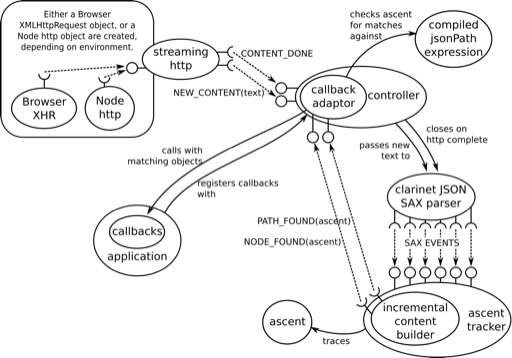
\includegraphics{images/overallDesign.png}
\caption{\textbf{Major components of Oboe.js illustrating program flow
from http transport to application callbacks.} UML facet/receptacle
notation is used to show the flow of events and event names are given in
capitals. For clarity events are depicted as transferring directly
between publisher and subscriber but this is actually performed through
an intermediary. \label{overallDesign}}
\end{figure}

Oboe's architecture describes a fairly linear pipeline visiting a small
number of tasks between receiving http content and notifying application
callbacks. The internal componentisation is designed primarily so that
automated testing can provide a high degree of confidence regarding the
correct working of the library. A local event bus facilitates
communication inside the Oboe instance and most components interact
solely by using this bus; receiving events, processing them, and
publishing further events in response. The use of an event bus is a
variation on the Observer pattern which removes the need for each unit
to locate specific other units before it may listen to their events,
giving a highly decoupled shape to the library in which each part knows
the events it requires but not who publishes them. Once everything is
wired into the bus no central control is required and the larger
behaviours emerge as the consequence of interaction between finer ones.

\subsection{Design for automated testing}

\begin{figure}[htbp]
\centering
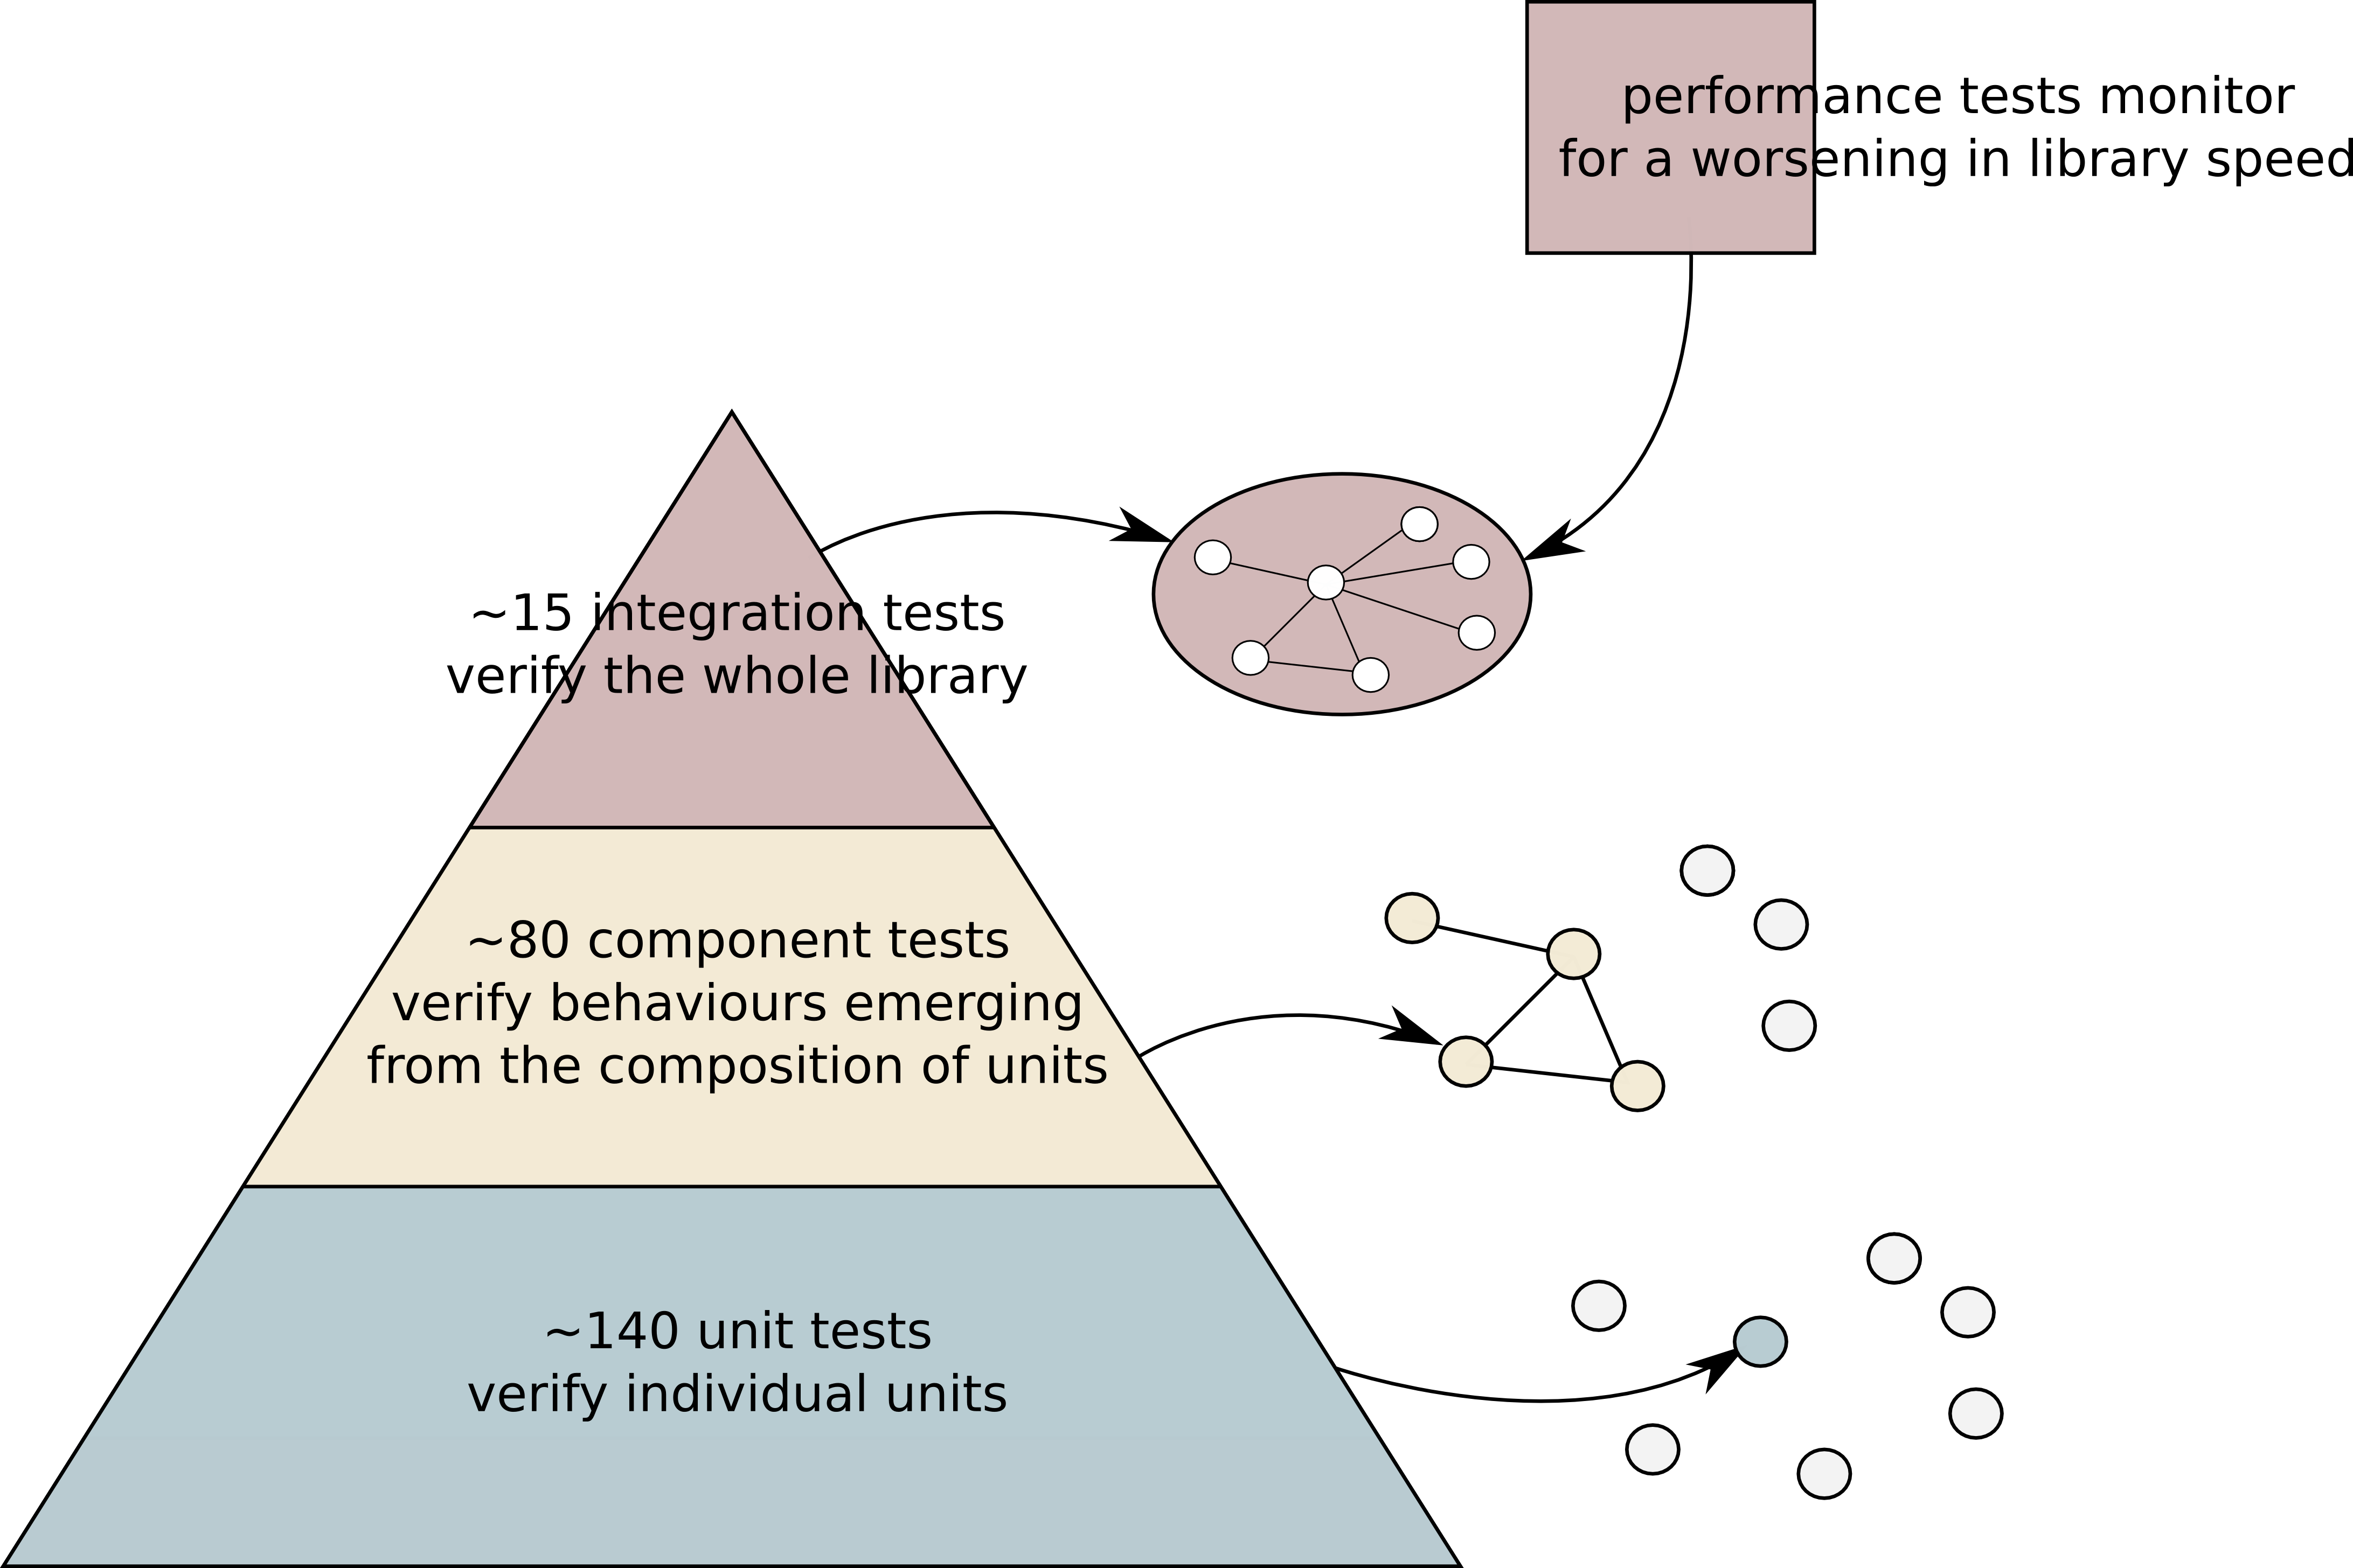
\includegraphics{images/testPyramid.png}
\caption{\textbf{The test pyramid}. Much testing is done on the
low-level components of the system, less on their composed behaviours,
and less still on a whole-system level. \label{testpyramid}}
\end{figure}

80\% of the code written for this project is test specification. Because
the correct behaviour of a composition requires the correct behaviour of
its components, the majority are \emph{unit tests}. The general style of
a unit test is to plug the item under test into a mock event bus and
check that when it receives input events the expected output events are
consequently published.

The \emph{Component tests} step back from examining individual
components to a position where their behaviour as a composition may be
examined. Because the compositions are quite simple there are fewer
component tests than unit tests. The component tests do not take account
of \emph{how} the composition is drawn and predominantly examine the
behaviour of the library through its public API. One exception is that
the streamingXHR component is switched for a stub so that http traffic
can be simulated.

At the apex of the test pyramid are a small number of \emph{integration
tests}. These verify Oboe as a black box without any knowledge of, or
access to, the internals, using the same API as is exposed to
application programmers. These tests are the most expensive to write but
a small number are necessary in order to verify that Oboe works
correctly end-to-end. Without access to the internals http traffic
cannot be faked so before these tests can be performed a corresponding
REST service is started. This test service is written using Node and
returns known content progressively according to predefined timings,
somewhat emulating a slow internet connection. The integration tests
particularly verify behaviours where platform differences could cause
inconsistencies. For example, the test url \texttt{/tenSlowNumbers}
writes out the first ten natural numbers as a JSON array at a rate of
two per second. The test registers a JSONPath selector that matches the
numbers against a callback that aborts the http request on seeing the
fifth. The correct behaviour is to get no sixth callback, even when
running on a platform lacking support for XHR2 and all ten will have
already been downloaded.

Confidently black-box testing a stateful unit is difficult. Because of
side-effects and hidden state we do not know if the same call will later
give a different behaviour. Building up the parse result from SAX events
is a fairly complex process which cannot be implemented efficiently as
stateless Javascript. To promote testability the state is delegated to a
simple state-storing unit. The intricate logic may then be expressed as
a separately tested set of side-effect free functions which transition
between one state and the next. Although proof of correctness is
impossible, for whichever results the functions give while under test,
uninfluenced by state I can be confident that they will always yield the
same response given the same future events. The separate unit
maintaining the state has exactly one responsibility, to hold the parse
result between function calls, and is trivial to test. This approach
slightly breaks with the object oriented principle of encapsulation by
hiding state behind the logic which acts on it but I feel that the
departure is justified by the more testable codebase.

To enhance testability Oboe has also embraced dependency injection.
Components do not instantiate their dependencies but rather rely on them
being passed in by an inversion of control container during the wiring
phase. For example, the network component which hides browser
differences does not know how to create the underlying XHR that it
adapts. Undoubtedly, by not instantiating its own transport this
component presents a less friendly interface: it's data source is no
longer a hidden implementation detail but exposed as a part of the it's
API at the responsibility of the caller. I feel this is mitigated by the
interface being purely internal. Dependency injection in this case
allows the tests to be written more simply because it is easy to
substitute the real XHR for a stub. Unit tests should test exactly one
unit, were the streaming http object to create its own transport, the
XHR would also be under test, plus whichever external service it
connects to. Because Javascript allows redefinition of built in types
the stubbing could have potentially also be done by overwriting the XHR
constructor to return a mock. However this is to be avoided as it opens
up the possibility of changes to the environment leaking between test
cases.

\subsection{Running the tests}

\begin{figure}[htbp]
\centering

\includegraphics{images/placeholder.png}
\caption{\textbf{Relationship between various files and test libraries}
\emph{other half of sketch from notebook}}
\end{figure}

The Grunt task runner is used to automate routine tasks such as
executing the tests and building, configured so that the unit and
component tests run automatically whenever a change is made to a source
file or specification. As well as executing correctly, the project is
required not to surpass a certain size so this also checked on every
save. Because Oboe is a small, tightly focused project the majority of
the programming time is spent refactoring already working code. Running
tests on save provides quick feedback so that mistakes are found before
my mind has moved on to the next context. Agile practitioners emphasise
the importance of tests that execute quickly (Martin 2008 p.314:T9) --
Oboe's 220 unit and component tests run in less than a second so
discovering programming mistakes is almost instant. If the ``content of
any medium is always another medium'' (McLuhan 1964 p.8), we might say
that the content of programming is the process that is realised by its
execution. A person working in a physical medium sees the thing they are
making but the programmer does usually not see their program's execution
simultaneously as they create. Conway notes that an artisan works by
transform-in-place ``start with the working material in place and you
step by step transform it into its final form,'' but software is created
through intermediate proxies. He attempts to close this gap by merging
programming with the results of programming (Conway 2004 pp.8-9). I feel
that if we bring together the medium and the message by viewing the
result of code while we write it, we can build as a series of small,
iterative, correct steps and programming can be more explorative and
expressive. Running the tests subtly, automatically hundreds of times
per day builds isn't merely convenient, this build process makes me a
better programmer.

Integration tests are not run on save. They intentionally simulate a
slow network so they take some time to run and I'd already have started
the next micro-task by the time they complete. Oboe is version
controlled using git and hosted on github. The integration tests are
used as the final check before a branch in git is merged into the
master.

\subsection{Packaging to a single distributable file}

As an interpreted language Javascript may be run without any prior
compilation. Directly running the files that are open in the editor is
convenient while programming but, unless a project is written as a
single file, in practice some build phase is required to create an
easily distributable form. Dependency managers have not yet become
standard for client-side web development so dependant libraries are
usually manually downloaded. For a developer wishing to include my
library in their own project a single file is much more convenient than
the multi-file raw source. If they are not using a similar build process
on their site, a single file is also faster to transfer to their users,
mostly because the http overhead is of constant size per resource.

Javascript files are interpreted in series by the browser so load-time
dependencies must precede dependants. If several valid Javascript files
are concatenated in the same order as delivered to the browser, the
joined version is functionally equivalent to the individual files. This
is a common technique so that code can be written and debugged as many
files but distributed as one. Several tools exist to automate this stage
of the build process that topologically sort the dependency graph before
concatenation in order to find a suitable script order.

Early in the project I chose \emph{Require.js} for this task. Javascript
as a language doesn't have an import statement. Require contributes the
importing ability to Javascript from inside the language itself by
providing an asynchronous \texttt{require} function. Calls to
\texttt{require} AJAX in and execute the imported source, passing any
exported items to the given callback. For non-trivial applications
loading each dependency individually over AJAX is intended only for
debugging because making so many requests is slow. For efficient
delivery Require also has the \texttt{optimise} command which
concatenates an application into a single file by using static analysis
to deduce a workable source order. Because the \texttt{require} function
may be called from anywhere, this is undecidable in the general case so
Require falls back to lazy loading. In practice this isn't a problem
because imports are generally not subject to branching. For larger
webapps lazy loading is a feature because it speeds up the initial page
load. The technique of \emph{Asynchronous Module Definition} (AMD)
intentionally imports rarely-loaded modules in response to events; by
resisting static analysis the dependant Javascript will not be
downloaded until it is needed. AMD is mostly of interest to applications
with a central hub but also some rarely used parts. For example, most
visits to online banking will not need to create standing orders so it
is better if this part is loaded on-demand rather than increase the
initial page load time.

I hoped to use Require's \texttt{optimise} to automate the creation of a
combined Javascript file for Oboe. Oboe would not benefit from AMD
because everybody who uses it will use all of the library but using
Require to find a working source order would save having to manually
implement one. Unfortunately this was not feasible. Even after
optimisation, Require's design necessitates that calls to the
\texttt{require} function are left in the code and that the Require
run-time component is available to handle them. At more than 5k gzipped
this would have more than doubled Oboe's download footprint.

After removing Require I decided to pick up the simplest tool which
could possibly work. With about 15 source files and a fairly sparse
dependency graph finding a working order on paper wasn't a daunting
task. Combined with a Grunt analogue to the unix \texttt{cat} command I
quickly had a working build process and a distributable library
requiring no run-time dependency management to be loaded.

For future consideration there is Browserify. This library reverses the
`browser first' Javascript mindset by viewing Node as the primary target
for Javascript development and adapting the browser environment to
match. Browserify converts applications written for Node into a single
file packaged for delivery to a web browser. Significantly, other than
Adaptors wrapping the browser APIs and presenting their features as if
they were the Node equivalents, Browserify leaves no trace of itself in
the final Javascript. Additionally, the http adaptor\footnote{\href{https://github.com/substack/http-browserify}{Https://github.com/substack/http-browserify}.}
is capable of using XHRs as a streaming source when used with supporting
browsers.

After combining into a single file Javascript source can be made
significantly smaller by \emph{minification} techniques such as reducing
scoped symbols to a single character or deleting the comments. For Oboe
the popular minifier library \emph{Uglify} was chosen. Uglify performs
only surface optimisations, concentrating mostly on producing compact
syntax by manipulating the code's abstract syntax tree. I also
considered Google's \emph{Closure Compiler} which resembles a
traditional optimiser by leveraging a deeper understanding of the code
semantics. Unfortunately, proving equivalence in highly dynamic
languages is often impossible and Closure Compiler is only safe given a
well-advised subset of Javascript. It delivers no reasonable guarantee
of equivalence if code is not written as the Closure team expected.
Integration tests would catch any such failures but for the time being I
decided that even given the micro-library limits, a slightly larger file
is a worthwhile tradeoff for a safer build process

\subsection{Styles of programming}

Oboe does not follow any single paradigm and is written as a mix of
procedural, functional and object-oriented programming styles. Classical
object orientation is used only so far as the library exposes an
Object-oriented public API. Although Javascript supports them, classes
and constructors are not used, nor is there any inheritance or notable
polymorphism. Closures form the primary means of data storage and
hiding. Most entities do not give a Javascript object on instantiation,
they are constructed as a set of event handlers with access to shared
values from a common closure. As inner-functions of the same containing
function, the handlers share access to variables from the containing
scope. From outside the closure the values are not only protected as
private as would be seen in an OO model, they are inherently
unaddressable.

Although not following an established object orientated metamodel, the
high-level componentisation hasn't departed very far from what I would
make were I following that style and OO design patterns have influenced
their layout considerably. If we wished to think in terms of the OO
paradigm we might say that values trapped inside closures are private
attributes and that the handlers registered on the event bus are public
methods. In this regard, the high-level internal design of Oboe can be
discussed using the terms from a more standard object oriented
metamodel.

Even where it creates a larger deliverable library I have generally
preferred writing as short functions which are combined to form longer
ones. Writing shorter functions reduces the size of the minimum testable
unit which, because each test can test a very small unit of
functionality, encourages very simple unit tests. Because the tests are
simple there is less room for unanticipated cases to hide. Due to
pressures on code size I decided not to use a general purpose functional
library and created my own with only the parts that are needed. See
\hyperref[functional.js]{functional.js} (Appendix
p.\pageref{functional.js}). Functional programming in Javascript is
known to be slower than other styles, particularly in Firefox which
lacks optimisations such as Lambda Lifting (Guo 2013). I do not think
this should be a major problem. Because of its single-threaded execution
model, in the browser any Javascript is ran during script execution
frames, interlaced with frames for other concurrent concerns. To
minimise the impact on other concerns such as rendering it is important
that no task occupies the CPU for very long. Since most monitors refresh
at 60Hz, about 16ms is a fair target for the maximum duration of a
script frame. In Node no limit can be implied from a display but any
CPU-hogging task degrades the responsiveness of concurrent concerns.
Switching tasks is cheap so sharing the CPU well generally prefers many
small execution frames over a few larger ones. Whether running in a
browser or server, the bottleneck is more often I/O than processing
speed; providing no task contiguously holds the CPU for an unusually
long time an application can usually be considered fast enough. Oboe's
progressive model favours sharing because it naturally splits the work
over many execution frames which by a non-progressive mode would be
performed during a single frame. Although the overall CPU time will be
higher, Oboe should share better with other concerns and because of
better I/O management the total system performance should be improved.

\subsection{Incrementally building the parsed content}

As shown in figure \ref{overallDesign} on page \pageref{overallDesign},
there is an \emph{incremental content builder} and \emph{ascent tracer}
which handle SAX events from the Clarinet JSON parser. By presenting to
the controller a simpler interface than is provided by Clarinet, taken
together these might be considered as an Adaptor pattern, albeit
modified to be even-driven rather than call-driven: we receive six event
types and in response emit from a vocabulary of two,
\texttt{NODE\_FOUND} and \texttt{PATH\_FOUND}. The events from Clarinet
are low level, reporting the sequence of tokens in the markup; those
emitted are at a much higher level of abstraction, reporting the JSON
nodes and paths as they are discovered. Testing a JSONPath expression
for a match against any particular node requires the node itself, the
path to the node, and the ancestor nodes. For each newly found item in
the JSON this information is delivered as the payload of the two event
types emitted by the content builder. When the callback adaptors receive
these events they have the information required to test registered
patterns for matches and notify application callbacks if required.

\begin{figure}[htbp]
\centering
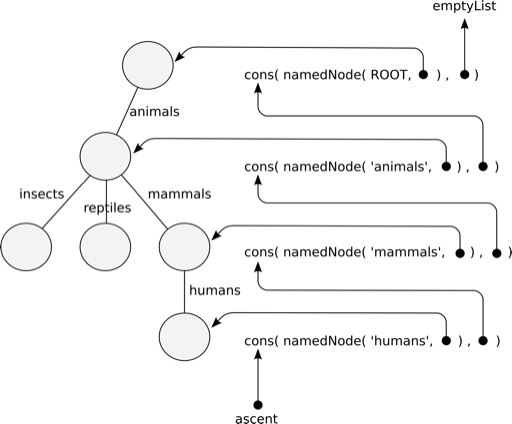
\includegraphics{images/ascent.png}
\caption{\textbf{List representation of an ascent rising from leaf to
root through a JSON tree.} Note the special ROOT value which represents
the location of the pathless root node. The ROOT value is an object,
taking advantage of object uniqueness to ensure that its location is
unequal to all others. \label{ascent}}
\end{figure}

The path to the current node is maintained as a singly linked list in
which each item holds the node and the field name that links to the node
from its parent. Each link in the list is immutable, enforced in newer
Javascript engines by using frozen objects.\footnote{See
  \url{https://developer.mozilla.org/en-US/docs/Web/JavaScript/Reference/Global\textbackslash{}_Objects/Object/freeze}.
  Although older engines don't provide any ability to create immutable
  objects, we can be fairly certain that the code does not mutate these
  objects or the tests would fail with attempts to modify in
  environments which are able to enforce it.} The list is arranged as an
ascent with the current node at the near end and the root at the far
end. Although paths are typically written as a \emph{descent}, ordering
as an \emph{ascent} is more efficient because every SAX event can be
processed in constant time by adding to or removing from the head of the
list. For familiarity, where paths are passed to application callbacks
they are first reversed and converted to arrays.

For each Clarinet event the builder provides a corresponding handler
which, working from the current ascent, returns the next ascent after
the event has been applied. For example, the \texttt{objectopen} and
\texttt{arrayopen} event types are handled by adding a new item at the
head of the ascent but for \texttt{closeobject} and \texttt{closearray}
one is removed. Over the course of parsing a JSON resource the ascent
will in this way be manipulated to visit every node, allowing each to be
tested against the registered JSONPath expressions. Internally, the
builder's handlers for SAX events are declared as the combination of a
smaller number of basic reusable parts. Several of Clarinet's event
types differ only by the type of the node that they announce but the
builder is largely unconcerned regarding a JSON node's type. On picking
up \texttt{openobject} and \texttt{openarray} events, both pass through
to the same \texttt{nodeFound} function, differing only in the type of
the node which is first created. Similarly, Clarinet emits a
\texttt{value} event when a string or number is found in the markup.
Because primitive nodes are always leaves the builder treats them as a
node which instantaneously starts and ends, handled programmatically as
the composition of the \texttt{nodeFound} and \texttt{nodeFinished}
functions.

Although the builder functions are stateless and side-effect free, while
visiting each JSON node the current ascent needs to be stored. This is
handled by the ascent tracker which serves as a holder for this data.
Starting with the ascent initialised as an empty list, on receiving a
SAX event it passes the ascent to the handler and stores the result so
that when the next SAX event is received the updated ascent can be given
to the next handler.

For the ascents linked lists were chosen in preference to the more
conventional approach of using native Javascript Arrays for several
reasons. Firstly, I find the program more easy to test and debug given
immutable data structures. Employing native Arrays without mutating
would be very expensive because on each new path the whole array would
have to be copied. Secondly, while debugging, unpicking a stack trace is
easier if I know that every value revealed is the value that has always
occupied that space and I don't have to project along the time axis by
imagining which values were in the same space earlier or will be later.
Thirdly, the lack of side effects means that I can try new commands in
the debugger's CLI without worrying about breaking the execution of the
program. Most Javascript virtual machines are also quite poor at array
growing and shrinking so for collections whose size changes often,
arrays are relatively inperformant. Finally, lists are a very convenient
format for the JSONPath engine to match against as will be discussed in
the next section. The Javascript file \hyperref[lists.js]{lists.js}
(Appendix p.\pageref{lists.js}) implements various list functions:
\texttt{cons}, \texttt{head}, \texttt{tail}, \texttt{map},
\texttt{foldR}, \texttt{all}, \texttt{without} as well as providing
conversions to and from arrays.

\subsection{Oboe JSONPath implementation}

On the first commit the JSONPath implementation was little more than a
series of regular expressions\footnote{JSONPath compiler from the first
  commit can be found at line 159 here:
  \url{https://github.com/jimhigson/oboe.js/blob/a17db7accc3a371853a2a0fd755153b10994c91e/src/main/progressive.js}\#L159
  for contrast, the current source can be found
  \hyperref[jsonPath.js]{in the appendix} on page \pageref{src_jsonPath}
  or at
  \url{https://github.com/jimhigson/oboe.js/blob/master/src/jsonPath.js}.}
but has slowly evolved into a featureful and efficient implementation.
The extent of the rewriting was possible because the correct behaviour
is well defined by test specifications\footnote{The current tests are
  viewable at
  \url{https://github.com/jimhigson/oboe.js/blob/master/test/specs/jsonPath.unit.spec.js}
  and
  \url{https://github.com/jimhigson/oboe.js/blob/master/test/specs/jsonPathTokens.unit.spec.js}.}.
The JSONPath compiler exposes a single higher-order function. This
function takes the JSONPath as a string and, proving it is a valid
expression, returns a function which tests for matches to the pattern.
The type of is difficult to express in Javascript but expressed as
Haskell would be:

\begin{Shaded}
\begin{Highlighting}[]
\DataTypeTok{String} \OtherTok{->} \DataTypeTok{Ascent} \OtherTok{->} \DataTypeTok{JsonPathMatchResult}
\end{Highlighting}
\end{Shaded}

The match result is either a hit or a miss. If a hit, the return value
is the node captured by the match. Should the pattern have an explicitly
capturing clause the node corresponding to that clause is captured,
otherwise it is the node at the head of the ascent. Implementation as a
higher-order function was chosen even though it might have been simpler
to create a first-order version as seen in the original JSONPath
implementation:

\begin{Shaded}
\begin{Highlighting}[]
\NormalTok{(}\DataTypeTok{String}\NormalTok{, }\DataTypeTok{Ascent}\NormalTok{) }\OtherTok{->} \DataTypeTok{JsonPathMatchResult}
\end{Highlighting}
\end{Shaded}

This version was rejected because the pattern string would have to be
freshly reinterpreted on each evaluation, repeating computation
unnecessarily. Because a pattern is registered once but then evaluated
perhaps hundreds of times per JSON file the most pressing performance
consideration is for matching to execute quickly. The extra time needed
to compile a pattern when new application callbacks are registered is
relatively insignificant because it is performed much less often.

The compilation is performed by recursively by examining the left-most
side of the string for a JSONPath clause. For each clause type there is
a function which tests ascents for that clause, for example by checking
the field name; by partial completion the field name function would be
specialised to match against one particular name. Having generated a
function to match against the left-most clause, compilation continues
recursively by passing itself the remaining unparsed right-side of the
string. The recursion continues until the terminal case where there is
nothing left to parse. On each recursive call the clause function
generated wraps the result from the last recursive call, resulting
ultimately in a concentric series of clause functions. The order of
these functions mirrors the ordering of paths as an ascent, so that the
outermost function matches against the node at the near end of the
ascent, and the innermost against the far end. When evaluated against an
ascent, each clause function examines the head of the list and, if it
matches, passes the list onto the next function. A special clause
function, \texttt{skip1} is used for the \texttt{.} (parent) syntax and
places no condition on the head of the list, unconditionally passing the
tail on to the next clause, thus moving matching on to the parent node.
Similarly, there is a function \texttt{skipMany} which maps onto the
\texttt{..} (ancestor) syntax and recursively consumes the minimum
number of ascent items necessary for the next clause to match or fails
if this cannot be done. In this way, we peel off layers from the ascent
as we move through the function list until we either exhaust the
functions, indicating a match, or cannot continue, indicating a fail.

This JSONPath implementation allows the compilation of complex
expressions into an executable form by combining many very simple
functions. As an example, the pattern
\texttt{!.\$person..\{height tShirtSize\}} once compiled would resemble
the Javascript functional representation below:

\begin{Shaded}
\begin{Highlighting}[]
\FunctionTok{statementExpr}\NormalTok{(             }\CommentTok{// outermost wrapper, added when JSONPath }
                           \CommentTok{//    is zero-length }
   \FunctionTok{duckTypeClause}\NormalTok{(         }\CommentTok{// token 5, \{height tShirtSize\}}
      \FunctionTok{skipMany}\NormalTok{(            }\CommentTok{// token 4, '..', ancestor relationship }
         \FunctionTok{capture}\NormalTok{(          }\CommentTok{// token 3, '$' from '$person'}
            \FunctionTok{nameClause}\NormalTok{(    }\CommentTok{// token 3, 'person' from '$person'}
               \FunctionTok{skip1}\NormalTok{(      }\CommentTok{// token 2, '.', parent relationship}
                  \NormalTok{rootExpr }\CommentTok{// token 1, '!', matches only the root}
               \NormalTok{) }
            \StringTok{'person'} \NormalTok{)}
         \NormalTok{)}
   \NormalTok{), [}\StringTok{'height'}\NormalTok{, }\StringTok{'tShirtSize'}\NormalTok{])}
\NormalTok{)      }
\end{Highlighting}
\end{Shaded}

Since I am using a side-effect free subset of Javascript for pattern
matching it would be safe to use a functional cache. As well as saving
time by avoiding repeated execution this could potentially also save
memory because where two JSONPath strings contain a common left side
they could share the inner part of their functional expression. Given
the patterns \texttt{!.animals.mammals.human} and
\texttt{!.animals.mammals.cats}, the JSONPath engine will currently
create two identical evaluators for \texttt{!.animals.mammals}.
Likewise, while evaluating of a pattern that requires matches at
multiple depths in the JSON hierarchy against sibling elements, the same
JSONPath evaluator term could be tested against the parent element many
times, always with the same result. Although Javascript doesn't come
with functional caching, it can be added using the language itself,
probably the best known example being \texttt{memoize} from
Underscore.js. I suspect, however, that hashing the cache parameters
might be slower than performing the matching. Although the parameters
are all immutable and could in theory be hashed by object identity, in
practice there is no way to access an object id from inside the language
so any hash of a node parsed out of JSON would have to walk the entire
subtree rooted from that node. Current Javascript implementations also
make it difficult to manage caches in general from inside the language
because there is no way to occupy only spare memory. Weak references are
proposed in ECMAScript 6 but currently only experimentally
supported\footnote{At time of writing, Firefox is the only engine
  supporting WeakHashMap by default. In Chome it is implemented but not
  available to Javascript unless explicitly enabled by a browser flag.
  \url{https://developer.mozilla.org/en-US/docs/Web/JavaScript/Reference/Global\textbackslash{}_Objects/WeakMap}
  retrieved 11th October 2013.}. If the hashing problem were solved, for
adding functional caching in future the WeakHashMap would be ideal.

Functions describing the tokenisation of the JSONPath language are split
out to their own source file and tested independently of the
compilation. Regular expressions are used because they are the simplest
form able to express the clause patterns. Each regular expressions
starts with \texttt{\^{}} so that they only match at the head of the
string, the `y' flag would be a more elegant alternative but as of now
this lacks wider browser support\footnote{\href{https://developer.mozilla.org/en-US/docs/Web/JavaScript/Guide/Regular\textbackslash{}_Expressions}{Https://developer.mozilla.org/en-US/docs/Web/JavaScript/Guide/Regular\textbackslash{}\_Expressions}.}.
By verifying the tokenisation functions through their own tests it is
simpler to create thorough specification because the tests may focus on
the tokenisation more clearly without having to observe its results
though another layer. For JSONPath matching we might consider the unit
test layer of the test pyramid (figure \ref{testpyramid}
p.\pageref{testpyramid}) is split further into two sub-layers. Arguably,
the upper of these sub-layers is not a unit test because it is verifying
more than one unit, the tokeniser and the compiler, and there is some
redundancy since the tokenisation is tested both independently and
through a proxy. However, a more purist approach would not be any more
useful because stubbing out the tokeniser functions before testing the
compiler would be a considerable effort and I do not believe it would
improve the rigor of the JSONPath specification.

\section{Conclusion}

\subsection{Differences in programs written using Oboe.js}

A program written using Oboe.js will be subtly different from one
written using more conventional libraries, even if the programmer means
to express the same thing. Consider the two examples below which use
Node.js to read a local JSON file and write to the console.

\begin{Shaded}
\begin{Highlighting}[]
\FunctionTok{oboe}\NormalTok{( }\OtherTok{fs}\NormalTok{.}\FunctionTok{createReadStream}\NormalTok{( }\StringTok{'/home/me/secretPlans.json'} \NormalTok{) )}
   \NormalTok{.}\FunctionTok{on}\NormalTok{(}\StringTok{'node'}\NormalTok{, \{}
      \StringTok{'schemes.*'}\NormalTok{: }\KeywordTok{function}\NormalTok{(scheme)\{}
         \OtherTok{console}\NormalTok{.}\FunctionTok{log}\NormalTok{(}\StringTok{'Aha! '} \NormalTok{+ scheme);}
      \NormalTok{\},}
      \StringTok{'plottings.*'}\NormalTok{: }\KeywordTok{function}\NormalTok{(deviousPlot)\{}
         \OtherTok{console}\NormalTok{.}\FunctionTok{log}\NormalTok{(}\StringTok{'Hmmm! '} \NormalTok{+ deviousPlot);}
      \NormalTok{\}   }
   \NormalTok{\})}
   \NormalTok{.}\FunctionTok{on}\NormalTok{(}\StringTok{'done'}\NormalTok{, }\KeywordTok{function}\NormalTok{()\{}
      \OtherTok{console}\NormalTok{.}\FunctionTok{log}\NormalTok{(}\StringTok{"*twiddles mustache*"}\NormalTok{);}
   \NormalTok{\})}
   \NormalTok{.}\FunctionTok{on}\NormalTok{(}\StringTok{'fail'}\NormalTok{, }\KeywordTok{function}\NormalTok{()\{}
      \OtherTok{console}\NormalTok{.}\FunctionTok{log}\NormalTok{(}\StringTok{"Drat! Foiled again!"}\NormalTok{);   }
   \NormalTok{\});}
\end{Highlighting}
\end{Shaded}

\begin{Shaded}
\begin{Highlighting}[]
\OtherTok{fs}\NormalTok{.}\FunctionTok{readFile}\NormalTok{(}\StringTok{'/home/me/secretPlans.json'}\NormalTok{, }\KeywordTok{function}\NormalTok{( err, plansJson )\{     }
   \KeywordTok{if}\NormalTok{( err ) \{}
      \OtherTok{console}\NormalTok{.}\FunctionTok{log}\NormalTok{(}\StringTok{"Drat! Foiled again!"}\NormalTok{);}
      \KeywordTok{return}\NormalTok{;}
   \NormalTok{\}}
   \KeywordTok{var} \NormalTok{plans = }\OtherTok{JSON}\NormalTok{.}\FunctionTok{parse}\NormalTok{(err, plansJson);}
   
   \OtherTok{plans}\NormalTok{.}\OtherTok{schemes}\NormalTok{.}\FunctionTok{forEach}\NormalTok{(}\KeywordTok{function}\NormalTok{( scheme )\{}
      \OtherTok{console}\NormalTok{.}\FunctionTok{log}\NormalTok{(}\StringTok{'Aha! '} \NormalTok{+ scheme);   }
   \NormalTok{\});   }
   \OtherTok{plans}\NormalTok{.}\OtherTok{plottings}\NormalTok{.}\FunctionTok{forEach}\NormalTok{(}\KeywordTok{function}\NormalTok{(deviousPlot)\{}
      \OtherTok{console}\NormalTok{.}\FunctionTok{log}\NormalTok{(}\StringTok{'Hmmm! '} \NormalTok{+ deviousPlot);}
   \NormalTok{\});}
      
   \OtherTok{console}\NormalTok{.}\FunctionTok{log}\NormalTok{(}\StringTok{"*twiddles mustache*"}\NormalTok{);   }
\NormalTok{\});}
\end{Highlighting}
\end{Shaded}

While the primary behaviours are similar, some accidental
side-behaviours differ between the two examples. It is likely the
programmer would not consider these differences as they write. In the
first example,the order of the output for schemes and plans will match
the order in the JSON, whereas for the second scheming is always done
before plotting. In the second example the order could be easily changed
by reversing the statements whereas the first id bound to echo the order
found in the JSON. The error behaviours are also different -- the first
prints until it has an error, the second prints if there are no errors.
In the second example it is \emph{almost mandatory} to check for errors
before output whereas in the first it feels most natural to register the
error listener at the end of the chained calls. I prefer the source
order in the first because the the normal case is listed before the
abnormal one. When describing a system, it seems odd to me to describe
the abnormal cases first.

Considering the coding style that is encouraged, the first example takes
a more declarative form by specifying the items of interest using
patterns whereas the second is more imperative by explicitly looping
through the items. If several levels of selection were required, such as
\texttt{schemes.*.steps.*}, other than a longer JSONPath pattern the
first example would not grow in complexity whereas the second would
require nested looping. We can say that the complexity of programming
using Oboe stays roughly constant whereas in the second example it grows
linearly with the number of levels that must be traversed.

\subsection{Benchmarking vs non-progressive REST}

I feel it is important to experimentally answer the question, \emph{is
this actually any faster?}. To measure performance I have created a
small benchmarking suite that runs under Node.js. One of my suggested
advantages of incremental parsing and perceptual improvement in speed. I
am not focusing on user perception for this evaluation because it would
be difficult to measure, requiring subjective judgement and human
participants. I will be measuring the time taken to provide the first
output which correlates with how quickly interface redrawing can start
and should give some indication as to perceptual speed. I chose Node to
host the tests because it is a minimalist platform which should give a
more repeatable results than browsers which could be performing any
number of simultaneous background tasks. Node also has the advantage
that small changes in memory use are not overwhelmed by a memory hungry
environment.

The benchmark mimics a REST service backed by a relational database.
Relational databases pass data from a result cursor one tuple at a time,
the service simulates this by writing out forty tuples as JSON objects,
one every ten milliseconds. Every other object in the returned JSON
contains a URL to a further resource which will also be fetched and an
aggregation created. To simulate real network conditions, Apple's
\emph{Network Line Conditioner} was used with the presets \emph{3G,
Average Case} and \emph{Cable modem} to represent poor and good internet
connections respectively.\footnote{\href{http://mattgemmell.com/2011/07/25/network-link-conditioner-in-lion/}{Http://mattgemmell.com/2011/07/25/network-link-conditioner-in-lion/}.}
The test involves two node processes, one acting as a REST client and
one as a REST server. Memory was measured on the client using Node's
built in memory reporting tool, \texttt{process.memoryusage()} and the
largest figure reported on each run is used. The test server and client
can be found in the project's \texttt{benchmark} directory, or in the
appendix on pages \ref{src_benchmarkServer} and
\ref{src_benchmarkClient}.

\begin{longtable}[c]{@{}llrrr@{}}
\hline\noalign{\medskip}
Client Strategy & Network & First output & Total time & Max. Memory
\\\noalign{\medskip}
\hline\noalign{\medskip}
Oboe.js & Good & 40ms & 804ms & 6.2Mb
\\\noalign{\medskip}
Oboe.js & Poor & 60ms & 1,526ms & 6.2Mb
\\\noalign{\medskip}
JSON.parse & Good & 984ms & 1,064ms & 9,0Mb
\\\noalign{\medskip}
JSON.parse & Poor & 2550ms & 2,609ms & 8.9Mb
\\\noalign{\medskip}
Clarinet & Good & 34ms & 781ms & 5.5Mb
\\\noalign{\medskip}
Clarinet & Poor & 52ms & 1,510ms & 5.5Mb
\\\noalign{\medskip}
\hline
\end{longtable}

In comparison with JSON.parse, Oboe shows a dramatic improvement of
about 96\% regarding the time taken for the first output and a smaller
but significant improvement of about 40\% in the total time required to
create the aggregation. Oboe's aggregation on a good network is about
15\% slower than Clarinet; since Oboe is built on Clarinet I did not
expect it to be faster but I had hoped for the gap to be smaller. This
is probably because Oboe encodes a more involved workflow than a raw SAX
parser.

Clarinet is known to be slower than JSON.parse for input which is
already held in memory\footnote{\href{http://writings.nunojob.com/2011/12/clarinet-sax-based-evented-streaming-json-parser-in-javascript-for-the-browser-and-nodejs.html}{Http://writings.nunojob.com/2011/12/clarinet-sax-based-evented-streaming-json-parser-in-javascript-for-the-browser-and-nodejs.html}.}
but when reading from a network this offset by the ability to parse
progressively. Compared to JSON.parse, the extra computation time needed
by Oboe is shown to be relatively insignificant in comparison to the
advantage of better i/o management. Reacting earlier using slower
handlers is shown to be faster overall than reacting later with quicker
ones. I believe that this vindicates the project focus on efficient
management of I/O over faster algorithms; much current programming takes
a ``Hurry up and wait'' approach by concentrating on small algorithm
optimisation over performing a task at the earliest possible time.

There is an unexpected improvement vs JSON.parse in terms of memory
usage. It is not clear why this would be but it may be attributable to
the large large dependency tree brought in by the get-json library which
was used to simplify this version. As expected, Clarinet has the
smallest memory usage because it never stores a complete version of the
parsed JSON. As REST resource size increases I would expect Clarinet's
memory usage to remain roughly constant while the other two rise
linearly. Node is popular on RaspberryPi type devices with constrained
RAM; Clarinet might be preferable to Oboe where code clarity is less
important than a small memory footprint

\subsection{Comparative developer ergonomics}

Writing less code is not in itself a guarantee of a better developer
ergonomics but I find it is a good indicator so long as the code isn't
forced to be overly terse. The code sizes below report the quantity of
code required to implement the benchmark REST client under each
strategy. Each version is written as the most natural expression for the
library used.

\begin{longtable}[c]{@{}lrr@{}}
\hline\noalign{\medskip}
Strategy & Code Required (lines) & Code required (chars)
\\\noalign{\medskip}
\hline\noalign{\medskip}
Oboe.js & 3 & 64
\\\noalign{\medskip}
JSON.parse & 5 & 102
\\\noalign{\medskip}
Clarinet & 30 & lots!
\\\noalign{\medskip}
\hline
\end{longtable}

Oboe was the shortest:

\begin{Shaded}
\begin{Highlighting}[]
\FunctionTok{oboe}\NormalTok{(DB_URL).}\FunctionTok{node}\NormalTok{(}\StringTok{'\{id url\}.url'}\NormalTok{, }\KeywordTok{function}\NormalTok{(url)\{}
   \FunctionTok{oboe}\NormalTok{(url).}\FunctionTok{node}\NormalTok{(}\StringTok{'name'}\NormalTok{, }\KeywordTok{function}\NormalTok{(name)\{}
      \OtherTok{console}\NormalTok{.}\FunctionTok{log}\NormalTok{(name);               }
   \NormalTok{\});      }
\NormalTok{\});}
\end{Highlighting}
\end{Shaded}

Non-progressive parsing with JSON.parse was slightly longer, requiring a
loop and an if statement, both to drill down into the results. The code
below is shortened by using the get-json\footnote{\href{https://npmjs.org/package/get-json}{Https://npmjs.org/package/get-json}.}
package which combines parsing implicitly into the download:

\begin{Shaded}
\begin{Highlighting}[]
\FunctionTok{getJson}\NormalTok{(DB_URL, }\KeywordTok{function}\NormalTok{(err, records) \{}
   \OtherTok{records}\NormalTok{.}\OtherTok{data}\NormalTok{.}\FunctionTok{forEach}\NormalTok{( }\KeywordTok{function}\NormalTok{( record )\{}
      \KeywordTok{if}\NormalTok{( }\OtherTok{record}\NormalTok{.}\FunctionTok{url} \NormalTok{) \{}
         \FunctionTok{getJson}\NormalTok{(}\OtherTok{record}\NormalTok{.}\FunctionTok{url}\NormalTok{, }\KeywordTok{function}\NormalTok{(err, record) \{}
            \OtherTok{console}\NormalTok{.}\FunctionTok{log}\NormalTok{(}\OtherTok{record}\NormalTok{.}\FunctionTok{name}\NormalTok{);}
         \NormalTok{\});}
      \NormalTok{\}}
   \NormalTok{\});}
\NormalTok{\});}
\end{Highlighting}
\end{Shaded}

This is tightly coupled with the JSON format that it reads. We can see
this in the fragments \texttt{records.data}, \texttt{record.url}, and
\texttt{record.name} which will only work if they find the desired
subtree at exactly the anticipated location. The code might be said to
contain a description of the format that it is for rather than a
description of what is required from the format. The Oboe version
describes the format only so far as is needed to identify the desired
parts; the remainder of the JSON could change and the code would
continue to work. I believe this demonstrates a greater tolerance to
changing formats and that this would be useful when programming against
evolving services.

The Clarinet version of the code is too long to include here but may be
seen \hyperref[header_benchmarkClient]{in the appendix}, on page
\pageref{src_benchmarkClient}. By using SAX directly the code is more
verbose and its purpose is obfuscated. I don't think a person looking at
this source could deduce what is being done without thinking about it
for some time. The functions receiving SAX events must handle several
different cases and so tend to have generic parameter names such as
`key' or `value' which represent the token type. By contrast, Oboe and
JSON.parse both allow names such as `record' or `url' which are chosen
according to the semantics of the value. I find this naming easier to
interpret because it allows me to think in terms of the domain model
rather than considering serialisation artifacts.

\subsection{Performance under various Javascript engines}

The file \texttt{oboe.performance.spec.js}\footnote{See
  \href{https://github.com/jimhigson/oboe.js/blob/master/test/specs/oboe.performance.spec.js}{tests/spec/oboe.performance.spec.js}.}
contains a benchmark which concentrates on using Oboe for pattern
matching. This test registers a complex pattern which intentionally uses
all features from the JSONPath language and then fetches a JSON file
containing approximately 800 nodes, 100 of which will match. Although
actual http is used, it is over an unthrottled connection to localhost
so network delay should be negligible. The tests are executed on a
relatively low-powered Macbook Air laptop running OS X 10.7.5, except
for Chrome Mobile which was tested on an iPhone 5 with iOS 7.0.2. Test
cases requiring Microsoft Windows were performed inside a VirtualBox
virtual machine. Curl is a simple download tool that writes the resource
to stdout without any parsing and is included as a baseline.

\begin{longtable}[c]{@{}lrr@{}}
\hline\noalign{\medskip}
Platform & Total Time & Throughput (nodes/ms)
\\\noalign{\medskip}
\hline\noalign{\medskip}
Curl & 42ms & \emph{unparsed, n/a}
\\\noalign{\medskip}
Chrome 31.0.1650.34 & 84ms & 9.57
\\\noalign{\medskip}
Node.js v0.10.1 & 172ms & 4.67
\\\noalign{\medskip}
Chrome 30.0.1599 & 202ms & 3.98
\\\noalign{\medskip}
Safari 6.0.5 & 231ms & 3.48
\\\noalign{\medskip}
IE 10.0.0 (Windows 8) & 349ms & 2.30
\\\noalign{\medskip}
Chrome Mobile iOS 30.0.1599 & 431ms & 1.86
\\\noalign{\medskip}
Firefox 24.0.0 & 547ms & 1.47
\\\noalign{\medskip}
IE 8.0.0 (Windows XP) & 3,048ms & 0.26
\\\noalign{\medskip}
\hline
\end{longtable}

We can see that Firefox is slower than other modern browsers despite
normally being quite fast. This is probably explicable by SpiderMonkey,
the Mozilla just-in-time Javascript compiler being poor at optimising
functional Javascript (Guo 2013). The JSON nodes are not of a common
type so many of the library's internal callsites are not monomorphic
which is also optimised poorly (Guo 2013). When the test was later
repeated with a simpler pattern Firefox showed by far the largest
improvement, indicating that the functional JSONPath matching accounts
for Firefox's lower than expected performance.

During the project version 31 of Chrome was released that performed more
than twice as quickly as the version 30 due to an updated version of the
v8 Javascript engine. Node also uses v8 and should catch up when it is
next updated. This reflects Javascript engine writers targeting
functional optimisation now that functional Javascript is becoming a
more popular style.

Of these results I find only the performance under old versions of
Internet Explorer poor enough to be concerning. Since this platform
cannot progressively interpret an XHR response an improvement over
traditional XHR was not possible, but I would have liked performance to
have not degraded by so much. Adding three seconds to a REST call will
unacceptably impair a webapp's user experience so it might be reasonable
to conclude that for complex use cases Oboe is currently unsuited to
legacy platforms. If we desired to improve performance on older
platforms one solution might be to create a simpler, non-progressive
implementation of the Oboe API for selective delivery to older browsers.
However, I would argue that time spent writing a basic legacy version
would be better spent waiting for these moribund platforms to die.

For an imperative language coded in a functional style the compiler may
not optimise as effectively as if a functional language were used. This
is especially the case for a highly dynamic language in which
everything, even the basic built-in types, are mutable. Presenting a
convenient API to application developers means passing eagerly evaluated
parameters to application callbacks even when the parameters are of
secondary importance and will be predominantly ignored. The the path and
ancestor arrays are created for every matching node but I anticipate
will be predominantly ignored. Under a functional language these could
be lazily evaluated without requiring any special effort by the
application programmer. I think Javascript was a good choice of
language, giving a very large number of client- and server-side
applications that may potentially adopt the library. However,
server-side Oboe would be very amicable to implementation using a purer
functional language and it would be interesting to see how much faster
it could be.

\subsection{Status as a micro-library}

The file \texttt{oboe-browser.min.js} is the minified, built version of
Oboe ready to be sent to web browsers and can be found in the project's
\texttt{dist} directory. The size fluctuates as commits are made but
after gzip it comes to about 4800 bytes; close to but comfortably under
the 5120 limit. At roughly the size as a small image the download
footprint of Oboe should not discourage adoption.

\subsection{Potential future work}

Although all network traffic can be viewed as a stream, the most obvious
future expansion would be to create a matching server-side component
that provides an intuitive interface for writing JSON streams. So far,
sending streaming JSON has required the resource be written out using
programmer-assembled strings but this approach is error prone and would
scale badly as messages become more complex. A stream-writer server side
library would allow Oboe to be used as a REST-compatible streaming
solution for situations which currently employ websockets. This would
provide a form of streaming that operates according to the principled
design of http rather than by sidestepping it.

There is nothing about Oboe that precludes working with other
tree-shaped formats. If there is demand, An XML/XPATH version seems like
an obvious expansion. This could be implemented by allowing resource
formats to be added using plugins which would allow programmers to
create a progressive interpretation of any resource type. As a minimum,
a plug-in would require a SAX-like parser and a compiler for some kind
of pattern matching language.

Oboe stores all JSON nodes that are parsed for the duration of its
lifetime so despite being similar to a SAX parser so far as it is
progressive, it consumes as much memory as a DOM parser. The nodes
remain held so that all possible JSONPath expressions may be tested.
However, in most cases memory could be freed if the parsed content were
stored only so far as is required to test against the patterns which
have actually been registered. For typical use cases I expect this would
allow large subtrees to be unlinked inside Oboe, particularly once they
have matched a pattern and have already been handed over to application
callbacks. Likewise, the current implementation takes a rather brute
force approach when examining nodes for pattern matches by checking
every registered JSONPath expression against every node parsed from the
JSON. For many expressions we should be able to say that there will be
no matches inside a particular JSON subtree, either because we have
already matched or because the the subtree's ancestors invariably imply
failure. A more sophisticated implementation might subdue provably
unsatisfiable handlers until the SAX parser leaves unmatchable subtrees.

\hyperdef{}{appendix_http_limits}{\section{Appendix i: Limits to number
of simultaneous connections under various http
clients}\label{appendix_http_limits}}

\begin{longtable}[c]{@{}ll@{}}
\hline\noalign{\medskip}
\begin{minipage}[b]{0.22\columnwidth}\raggedright
http Client
\end{minipage} & \begin{minipage}[b]{0.29\columnwidth}\raggedright
connection limit per server
\end{minipage}
\\\noalign{\medskip}
\hline\noalign{\medskip}
\begin{minipage}[t]{0.22\columnwidth}\raggedright
Firefox
\end{minipage} & \begin{minipage}[t]{0.29\columnwidth}\raggedright
6
\end{minipage}
\\\noalign{\medskip}
\begin{minipage}[t]{0.22\columnwidth}\raggedright
Internet Explorer
\end{minipage} & \begin{minipage}[t]{0.29\columnwidth}\raggedright
4
\end{minipage}
\\\noalign{\medskip}
\begin{minipage}[t]{0.22\columnwidth}\raggedright
Chrome / Chromium
\end{minipage} & \begin{minipage}[t]{0.29\columnwidth}\raggedright
32 sockets per proxy 6 sockets per destination host 256 sockets per
process
\end{minipage}
\\\noalign{\medskip}
\hline
\end{longtable}

\url{https://developer.mozilla.org/en-US/docs/Web/API/XMLHttpRequest}

\url{http://msdn.microsoft.com/de-de/magazine/ee330731.aspx}\#http11\_max\_con

\url{http://dev.chromium.org/developers/design-documents/network-stack}\#TOC-Connection-Management

\section{Appendix ii: Oboe.js source code listing}

\subsection{clarinetListenerAdaptor.js}

\label{src_clarinetListenerAdaptor}

\begin{Shaded}
\begin{Highlighting}[]

\CommentTok{/** }
\CommentTok{ * A bridge used to assign stateless functions to listen to clarinet.}
\CommentTok{ * }
\CommentTok{ * As well as the parameter from clarinet, each callback will also be passed}
\CommentTok{ * the result of the last callback.}
\CommentTok{ * }
\CommentTok{ * This may also be used to clear all listeners by assigning zero handlers:}
\CommentTok{ * }
\CommentTok{ *    clarinetListenerAdaptor( clarinet, \{\} )}
\CommentTok{ */}
\KeywordTok{function} \FunctionTok{clarinetListenerAdaptor}\NormalTok{(clarinetParser, handlers)\{}
    
   \KeywordTok{var} \NormalTok{state;}

   \OtherTok{clarinet}\NormalTok{.}\OtherTok{EVENTS}\NormalTok{.}\FunctionTok{forEach}\NormalTok{(}\KeywordTok{function}\NormalTok{(eventName)\{}
 
      \KeywordTok{var} \NormalTok{handlerFunction = handlers[eventName];}
      
      \NormalTok{clarinetParser[}\StringTok{'on'}\NormalTok{+eventName] = handlerFunction && }
                                       \KeywordTok{function}\NormalTok{(param) \{}
                                          \NormalTok{state = }\FunctionTok{handlerFunction}\NormalTok{( state, param);}
                                       \NormalTok{\};}
   \NormalTok{\});}
\NormalTok{\}}
\end{Highlighting}
\end{Shaded}

\pagebreak

\subsection{events.js}

\label{src_events}

\begin{Shaded}
\begin{Highlighting}[]
\CommentTok{/**}
\CommentTok{ * This file declares some constants to use as names for event types.}
\CommentTok{ */}

\KeywordTok{var} \CommentTok{// NODE_FOUND, PATH_FOUND and ERROR_EVENT feature }
    \CommentTok{// in the public API via .on('node', ...) or .on('path', ...)}
    \CommentTok{// so these events are strings}
    \NormalTok{NODE_FOUND    = }\StringTok{'node'}\NormalTok{,  }
    \NormalTok{PATH_FOUND    = }\StringTok{'path'}\NormalTok{,   }
         
    \CommentTok{// these events are never exported so are kept as }
    \CommentTok{// the smallest possible representation, numbers:}
    \NormalTok{_S = }\DecValTok{0}\NormalTok{,}
    \NormalTok{ERROR_EVENT   = _S++,    }
    \NormalTok{ROOT_FOUND    = _S++,    }
    \NormalTok{NEW_CONTENT = _S++,}
    \NormalTok{END_OF_CONTENT = _S++,}
    \NormalTok{ABORTING = _S++;}
    
\KeywordTok{function} \FunctionTok{errorReport}\NormalTok{(statusCode, body, error) \{}
   \KeywordTok{try}\NormalTok{\{}
      \KeywordTok{var} \NormalTok{jsonBody = }\OtherTok{JSON}\NormalTok{.}\FunctionTok{parse}\NormalTok{(body);}
   \NormalTok{\}}\KeywordTok{catch}\NormalTok{(e)\{\}}

   \KeywordTok{return} \NormalTok{\{}
      \DataTypeTok{statusCode}\NormalTok{:statusCode,}
      \DataTypeTok{body}\NormalTok{:body,}
      \DataTypeTok{jsonBody}\NormalTok{:jsonBody,}
      \DataTypeTok{thrown}\NormalTok{:error}
   \NormalTok{\};}
\NormalTok{\}    }
\end{Highlighting}
\end{Shaded}

\pagebreak

\subsection{functional.js}

\label{src_functional}

\begin{Shaded}
\begin{Highlighting}[]
\CommentTok{/** }
\CommentTok{ * Partially complete a function.}
\CommentTok{ * }
\CommentTok{ * Eg: }
\CommentTok{ *    var add3 = partialComplete( function add(a,b)\{return a+b\}, 3 );}
\CommentTok{ *    }
\CommentTok{ *    add3(4) // gives 7}
\CommentTok{ *    }
\CommentTok{ *    }
\CommentTok{ *    function wrap(left, right, cen)\{return left + " " + cen + " " + right;\}}
\CommentTok{ *    }
\CommentTok{ *    var pirateGreeting = partialComplete( wrap , "I'm", ", a mighty pirate!" );}
\CommentTok{ *    }
\CommentTok{ *    pirateGreeting("Guybrush Threepwood"); }
\CommentTok{ *                         // gives "I'm Guybrush Threepwood, a mighty pirate!"}
\CommentTok{ */}
\KeywordTok{var} \NormalTok{partialComplete = }\FunctionTok{varArgs}\NormalTok{(}\KeywordTok{function}\NormalTok{( fn, boundArgs ) \{}

      \KeywordTok{return} \FunctionTok{varArgs}\NormalTok{(}\KeywordTok{function}\NormalTok{( callArgs ) \{}
               
         \KeywordTok{return} \OtherTok{fn}\NormalTok{.}\FunctionTok{apply}\NormalTok{(}\KeywordTok{this}\NormalTok{, }\OtherTok{boundArgs}\NormalTok{.}\FunctionTok{concat}\NormalTok{(callArgs));}
      \NormalTok{\}); }
   \NormalTok{\}),}


\CommentTok{/**}
\CommentTok{ * Compose zero or more functions:}
\CommentTok{ * }
\CommentTok{ *    compose(f1, f2, f3)(x) = f1(f2(f3(x))))}
\CommentTok{ * }
\CommentTok{ * The last (inner-most) function may take more than one parameter:}
\CommentTok{ * }
\CommentTok{ *    compose(f1, f2, f3)(x,y) = f1(f2(f3(x,y))))}
\CommentTok{ */}
   \NormalTok{compose = }\FunctionTok{varArgs}\NormalTok{(}\KeywordTok{function}\NormalTok{(fns) \{}

      \KeywordTok{var} \NormalTok{fnsList = }\FunctionTok{arrayAsList}\NormalTok{(fns);}
   
      \KeywordTok{function} \FunctionTok{next}\NormalTok{(params, curFn) \{  }
         \KeywordTok{return} \NormalTok{[}\FunctionTok{apply}\NormalTok{(params, curFn)];   }
      \NormalTok{\}}
      
      \KeywordTok{return} \FunctionTok{varArgs}\NormalTok{(}\KeywordTok{function}\NormalTok{(startParams)\{}
        
         \KeywordTok{return} \FunctionTok{foldR}\NormalTok{(next, startParams, fnsList)[}\DecValTok{0}\NormalTok{];}
      \NormalTok{\});}
   \NormalTok{\}),}

\CommentTok{/**}
\CommentTok{ * Call a list of functions with the same args until one returns a }
\CommentTok{ * truthy result. Similar to the \textbar{}\textbar{} operator.}
\CommentTok{ * }
\CommentTok{ * So:}
\CommentTok{ *      lazyUnion([f1,f2,f3 ... fn])( p1, p2 ... pn )}
\CommentTok{ *      }
\CommentTok{ * Is equivalent to: }
\CommentTok{ *      apply([p1, p2 ... pn], f1) \textbar{}\textbar{} }
\CommentTok{ *      apply([p1, p2 ... pn], f2) \textbar{}\textbar{} }
\CommentTok{ *      apply([p1, p2 ... pn], f3) ... apply(fn, [p1, p2 ... pn])  }
\CommentTok{ *  }
\CommentTok{ * }\KeywordTok{@returns}\CommentTok{ the first return value that is given that is truthy.}
\CommentTok{ */}
   \NormalTok{lazyUnion = }\FunctionTok{varArgs}\NormalTok{(}\KeywordTok{function}\NormalTok{(fns) \{}

      \KeywordTok{return} \FunctionTok{varArgs}\NormalTok{(}\KeywordTok{function}\NormalTok{(params)\{}
   
         \KeywordTok{var} \NormalTok{maybeValue;}
   
         \KeywordTok{for} \NormalTok{(}\KeywordTok{var} \NormalTok{i = }\DecValTok{0}\NormalTok{; i < }\FunctionTok{len}\NormalTok{(fns); i++) \{}
   
            \NormalTok{maybeValue = }\FunctionTok{apply}\NormalTok{(params, fns[i]);}
   
            \KeywordTok{if}\NormalTok{( maybeValue ) \{}
               \KeywordTok{return} \NormalTok{maybeValue;}
            \NormalTok{\}}
         \NormalTok{\}}
      \NormalTok{\});}
   \NormalTok{\});   }

\CommentTok{/**}
\CommentTok{ * This file declares various pieces of functional programming.}
\CommentTok{ * }
\CommentTok{ * This isn't a general purpose functional library, to keep things small it}
\CommentTok{ * has just the parts useful for Oboe.js.}
\CommentTok{ */}


\CommentTok{/**}
\CommentTok{ * Call a single function with the given arguments array.}
\CommentTok{ * Basically, a functional-style version of the OO-style Function#apply for }
\CommentTok{ * when we don't care about the context ('this') of the call.}
\CommentTok{ * }
\CommentTok{ * The order of arguments allows partial completion of the arguments array}
\CommentTok{ */}
\KeywordTok{function} \FunctionTok{apply}\NormalTok{(args, fn) \{}
   \KeywordTok{return} \OtherTok{fn}\NormalTok{.}\FunctionTok{apply}\NormalTok{(}\KeywordTok{undefined}\NormalTok{, args);}
\NormalTok{\}}

\CommentTok{/**}
\CommentTok{ * Define variable argument functions but cut out all that tedious messing about }
\CommentTok{ * with the arguments object. Delivers the variable-length part of the arguments}
\CommentTok{ * list as an array.}
\CommentTok{ * }
\CommentTok{ * Eg:}
\CommentTok{ * }
\CommentTok{ * var myFunction = varArgs(}
\CommentTok{ *    function( fixedArgument, otherFixedArgument, variableNumberOfArguments )\{}
\CommentTok{ *       console.log( variableNumberOfArguments );}
\CommentTok{ *    \}}
\CommentTok{ * )}
\CommentTok{ * }
\CommentTok{ * myFunction('a', 'b', 1, 2, 3); // logs [1,2,3]}
\CommentTok{ * }
\CommentTok{ * var myOtherFunction = varArgs(function( variableNumberOfArguments )\{}
\CommentTok{ *    console.log( variableNumberOfArguments );}
\CommentTok{ * \})}
\CommentTok{ * }
\CommentTok{ * myFunction(1, 2, 3); // logs [1,2,3]}
\CommentTok{ * }
\CommentTok{ */}
\KeywordTok{function} \FunctionTok{varArgs}\NormalTok{(fn)\{}

   \KeywordTok{var} \NormalTok{numberOfFixedArguments = }\OtherTok{fn}\NormalTok{.}\FunctionTok{length} \NormalTok{-}\DecValTok{1}\NormalTok{;}
         
   \KeywordTok{return} \KeywordTok{function}\NormalTok{()\{}
   
      \KeywordTok{var} \NormalTok{numberOfVaraibleArguments = }\OtherTok{arguments}\NormalTok{.}\FunctionTok{length} \NormalTok{- numberOfFixedArguments,}
      
          \NormalTok{argumentsToFunction = }\OtherTok{Array}\NormalTok{.}\OtherTok{prototype}\NormalTok{.}\OtherTok{slice}\NormalTok{.}\FunctionTok{call}\NormalTok{(arguments);}
          
      \CommentTok{// remove the last n element from the array and append it onto the end of}
      \CommentTok{// itself as a sub-array}
      \OtherTok{argumentsToFunction}\NormalTok{.}\FunctionTok{push}\NormalTok{( }
         \OtherTok{argumentsToFunction}\NormalTok{.}\FunctionTok{splice}\NormalTok{(numberOfFixedArguments, numberOfVaraibleArguments)}
      \NormalTok{);   }
      
      \KeywordTok{return} \OtherTok{fn}\NormalTok{.}\FunctionTok{apply}\NormalTok{( }\KeywordTok{this}\NormalTok{, argumentsToFunction );}
   \NormalTok{\}       }
\NormalTok{\}}


\CommentTok{/**}
\CommentTok{ * Swap the order of parameters to a binary function}
\CommentTok{ * }
\CommentTok{ * A bit like this flip: http://zvon.org/other/haskell/Outputprelude/flip_f.html}
\CommentTok{ */}
\KeywordTok{function} \FunctionTok{flip}\NormalTok{(fn)\{}
   \KeywordTok{return} \KeywordTok{function}\NormalTok{(a, b)\{}
      \KeywordTok{return} \FunctionTok{fn}\NormalTok{(b,a);}
   \NormalTok{\}}
\NormalTok{\}}


\CommentTok{/**}
\CommentTok{ * Create a function which is the intersection of two other functions.}
\CommentTok{ * }
\CommentTok{ * Like the && operator, if the first is truthy, the second is never called,}
\CommentTok{ * otherwise the return value from the second is returned.}
\CommentTok{ */}
\KeywordTok{function} \FunctionTok{lazyIntersection}\NormalTok{(fn1, fn2) \{}

   \KeywordTok{return} \KeywordTok{function} \NormalTok{(param) \{}
                                                              
      \KeywordTok{return} \FunctionTok{fn1}\NormalTok{(param) && }\FunctionTok{fn2}\NormalTok{(param);}
   \NormalTok{\};   }
\NormalTok{\}}

\end{Highlighting}
\end{Shaded}

\pagebreak

\subsection{incrementalContentBuilder.js}

\label{src_incrementalContentBuilder}

\begin{Shaded}
\begin{Highlighting}[]
\CommentTok{/** }
\CommentTok{ * This file provides various listeners which can be used to build up}
\CommentTok{ * a changing ascent based on the callbacks provided by Clarinet. It listens}
\CommentTok{ * to the low-level events from Clarinet and emits higher-level ones.}
\CommentTok{ *  }
\CommentTok{ * The building up is stateless so to track a JSON file}
\CommentTok{ * clarinetListenerAdaptor.js is required to store the ascent state}
\CommentTok{ * between calls.}
\CommentTok{ */}


\KeywordTok{var} \NormalTok{keyOf = }\FunctionTok{attr}\NormalTok{(}\StringTok{'key'}\NormalTok{);}
\KeywordTok{var} \NormalTok{nodeOf = }\FunctionTok{attr}\NormalTok{(}\StringTok{'node'}\NormalTok{);}


\CommentTok{/** }
\CommentTok{ * A special value to use in the path list to represent the path 'to' a root }
\CommentTok{ * object (which doesn't really have any path). This prevents the need for }
\CommentTok{ * special-casing detection of the root object and allows it to be treated }
\CommentTok{ * like any other object. We might think of this as being similar to the }
\CommentTok{ * 'unnamed root' domain ".", eg if I go to }
\CommentTok{ * http://en.wikipedia.org./wiki/En/Main_page the dot after 'org' deliminates }
\CommentTok{ * the unnamed root of the DNS.}
\CommentTok{ * }
\CommentTok{ * This is kept as an object to take advantage that in Javascript's OO objects }
\CommentTok{ * are guaranteed to be distinct, therefore no other object can possibly clash }
\CommentTok{ * with this one. Strings, numbers etc provide no such guarantee. }
\CommentTok{ **/}
\KeywordTok{var} \NormalTok{ROOT_PATH = \{\};}


\CommentTok{/**}
\CommentTok{ * Create a new set of handlers for clarinet's events, bound to the emit }
\CommentTok{ * function given.  }
\CommentTok{ */} 
\KeywordTok{function} \FunctionTok{incrementalContentBuilder}\NormalTok{( emit ) \{}


   \KeywordTok{function} \FunctionTok{arrayIndicesAreKeys}\NormalTok{( possiblyInconsistentAscent, newDeepestNode) \{}
   
      \CommentTok{/* for values in arrays we aren't pre-warned of the coming paths }
\CommentTok{         (Clarinet gives no call to onkey like it does for values in objects) }
\CommentTok{         so if we are in an array we need to create this path ourselves. The }
\CommentTok{         key will be len(parentNode) because array keys are always sequential }
\CommentTok{         numbers. */}

      \KeywordTok{var} \NormalTok{parentNode = }\FunctionTok{nodeOf}\NormalTok{( }\FunctionTok{head}\NormalTok{( possiblyInconsistentAscent));}
      
      \KeywordTok{return}      \FunctionTok{isOfType}\NormalTok{( Array, parentNode)}
               \NormalTok{?}
                  \FunctionTok{pathFound}\NormalTok{(  possiblyInconsistentAscent, }
                              \FunctionTok{len}\NormalTok{(parentNode), }
                              \NormalTok{newDeepestNode}
                  \NormalTok{)}
               \NormalTok{:  }
                  \CommentTok{// nothing needed, return unchanged}
                  \NormalTok{possiblyInconsistentAscent }
               \NormalTok{;}
   \NormalTok{\}}
                 
   \KeywordTok{function} \FunctionTok{nodeFound}\NormalTok{( ascent, newDeepestNode ) \{}
      
      \KeywordTok{if}\NormalTok{( !ascent ) \{}
         \CommentTok{// we discovered the root node,}
         \FunctionTok{emit}\NormalTok{( ROOT_FOUND, newDeepestNode);}
                    
         \KeywordTok{return} \FunctionTok{pathFound}\NormalTok{( ascent, ROOT_PATH, newDeepestNode);         }
      \NormalTok{\}}

      \CommentTok{// we discovered a non-root node}
                 
      \KeywordTok{var} \NormalTok{arrayConsistentAscent  = }\FunctionTok{arrayIndicesAreKeys}\NormalTok{( ascent, newDeepestNode),      }
          \NormalTok{ancestorBranches       = }\FunctionTok{tail}\NormalTok{( arrayConsistentAscent),}
          \NormalTok{previouslyUnmappedName = }\FunctionTok{keyOf}\NormalTok{( }\FunctionTok{head}\NormalTok{( arrayConsistentAscent));}
          
      \FunctionTok{appendBuiltContent}\NormalTok{( }
         \NormalTok{ancestorBranches, }
         \NormalTok{previouslyUnmappedName, }
         \NormalTok{newDeepestNode }
      \NormalTok{);}
                                                                                                         
      \KeywordTok{return} \FunctionTok{cons}\NormalTok{( }
               \FunctionTok{namedNode}\NormalTok{( previouslyUnmappedName, newDeepestNode ), }
               \NormalTok{ancestorBranches}
      \NormalTok{);                                                                          }
   \NormalTok{\}}


   \CommentTok{/**}
\CommentTok{    * Add a new value to the object we are building up to represent the}
\CommentTok{    * parsed JSON}
\CommentTok{    */}
   \KeywordTok{function} \FunctionTok{appendBuiltContent}\NormalTok{( ancestorBranches, key, node )\{}
     
      \FunctionTok{nodeOf}\NormalTok{( }\FunctionTok{head}\NormalTok{( ancestorBranches))[key] = node;}
   \NormalTok{\}}

   \CommentTok{/**}
\CommentTok{    * Get a new key->node mapping}
\CommentTok{    * }
\CommentTok{    * }\KeywordTok{@param}\CommentTok{ }\KeywordTok{\{String\textbar{}Number\}}\CommentTok{ key}
\CommentTok{    * }\KeywordTok{@param}\CommentTok{ }\KeywordTok{\{Object\textbar{}Array\textbar{}String\textbar{}Number\textbar{}null\}}\CommentTok{ node a value found in the json}
\CommentTok{    */}
   \KeywordTok{function} \FunctionTok{namedNode}\NormalTok{(key, node) \{}
      \KeywordTok{return} \NormalTok{\{}\DataTypeTok{key}\NormalTok{:key, }\DataTypeTok{node}\NormalTok{:node\};}
   \NormalTok{\}}
     
   \CommentTok{/**}
\CommentTok{    * For when we find a new key in the json.}
\CommentTok{    * }
\CommentTok{    * }\KeywordTok{@param}\CommentTok{ }\KeywordTok{\{String\textbar{}Number\textbar{}Object\}}\CommentTok{ newDeepestName the key. If we are in an }
\CommentTok{    *    array will be a number, otherwise a string. May take the special }
\CommentTok{    *    value ROOT_PATH if the root node has just been found}
\CommentTok{    *    }
\CommentTok{    * }\KeywordTok{@param}\CommentTok{ }\KeywordTok{\{String\textbar{}Number\textbar{}Object\textbar{}Array\textbar{}Null\textbar{}undefined\}}\CommentTok{ [maybeNewDeepestNode] }
\CommentTok{    *    usually this won't be known so can be undefined. Can't use null }
\CommentTok{    *    to represent unknown because null is a valid value in JSON}
\CommentTok{    **/}  
   \KeywordTok{function} \FunctionTok{pathFound}\NormalTok{(ascent, newDeepestName, maybeNewDeepestNode) \{}

      \KeywordTok{if}\NormalTok{( ascent ) \{ }\CommentTok{// if not root}
      
         \CommentTok{// If we have the key but (unless adding to an array) no known value}
         \CommentTok{// yet. Put that key in the output but against no defined value:      }
         \FunctionTok{appendBuiltContent}\NormalTok{( ascent, newDeepestName, maybeNewDeepestNode );}
      \NormalTok{\}}
   
      \KeywordTok{var} \NormalTok{ascentWithNewPath = }\FunctionTok{cons}\NormalTok{( }
                                 \FunctionTok{namedNode}\NormalTok{( newDeepestName, }
                                            \NormalTok{maybeNewDeepestNode), }
                                 \NormalTok{ascent}
                              \NormalTok{);}
     
      \FunctionTok{emit}\NormalTok{( PATH_FOUND, ascentWithNewPath);}
 
      \KeywordTok{return} \NormalTok{ascentWithNewPath;}
   \NormalTok{\}}


   \CommentTok{/**}
\CommentTok{    * For when the current node ends}
\CommentTok{    */}
   \KeywordTok{function} \FunctionTok{nodeFinished}\NormalTok{( ascent ) \{}

      \FunctionTok{emit}\NormalTok{( NODE_FOUND, ascent);}
                          
      \CommentTok{// pop the complete node and its path off the list:                                    }
      \KeywordTok{return} \FunctionTok{tail}\NormalTok{( ascent);}
   \NormalTok{\}      }
                 
   \KeywordTok{return} \NormalTok{\{ }

      \DataTypeTok{openobject }\NormalTok{: }\KeywordTok{function} \NormalTok{(ascent, firstKey) \{}

         \KeywordTok{var} \NormalTok{ascentAfterNodeFound = }\FunctionTok{nodeFound}\NormalTok{(ascent, \{\});         }

         \CommentTok{/* It is a perculiarity of Clarinet that for non-empty objects it}
\CommentTok{            gives the first key with the openobject event instead of}
\CommentTok{            in a subsequent key event.}
\CommentTok{                      }
\CommentTok{            firstKey could be the empty string in a JSON object like }
\CommentTok{            \{'':'foo'\} which is technically valid.}
\CommentTok{            }
\CommentTok{            So can't check with !firstKey, have to see if has any }
\CommentTok{            defined value. */}
         \KeywordTok{return} \FunctionTok{defined}\NormalTok{(firstKey)}
         \NormalTok{?          }
            \CommentTok{/* We know the first key of the newly parsed object. Notify that }
\CommentTok{               path has been found but don't put firstKey permanently onto }
\CommentTok{               pathList yet because we haven't identified what is at that key }
\CommentTok{               yet. Give null as the value because we haven't seen that far }
\CommentTok{               into the json yet */}
            \FunctionTok{pathFound}\NormalTok{(ascentAfterNodeFound, firstKey)}
         \NormalTok{:}
            \NormalTok{ascentAfterNodeFound}
         \NormalTok{;}
      \NormalTok{\},}
    
      \DataTypeTok{openarray}\NormalTok{: }\KeywordTok{function} \NormalTok{(ascent) \{}
         \KeywordTok{return} \FunctionTok{nodeFound}\NormalTok{(ascent, []);}
      \NormalTok{\},}

      \CommentTok{// called by Clarinet when keys are found in objects               }
      \DataTypeTok{key}\NormalTok{: pathFound,}
      
      \CommentTok{/* Emitted by Clarinet when primitive values are found, ie Strings,}
\CommentTok{         Numbers, and null.}
\CommentTok{         Because these are always leaves in the JSON, we find and finish the }
\CommentTok{         node in one step, expressed as functional composition: */}
      \DataTypeTok{value}\NormalTok{: }\FunctionTok{compose}\NormalTok{( nodeFinished, nodeFound ),}
      
      \CommentTok{// we make no distinction in how we handle object and arrays closing.}
      \CommentTok{// For both, interpret as the end of the current node.}
      \DataTypeTok{closeobject}\NormalTok{: nodeFinished,}
      \DataTypeTok{closearray}\NormalTok{: nodeFinished}
   \NormalTok{\};}
\NormalTok{\}}
\end{Highlighting}
\end{Shaded}

\pagebreak

\subsection{instanceController.js}

\label{src_instanceController}

\begin{Shaded}
\begin{Highlighting}[]
\CommentTok{/**}
\CommentTok{ * This file implements a light-touch central controller for an instance }
\CommentTok{ * of Oboe which provides the methods used for interacting with the instance }
\CommentTok{ * from the calling app.}
\CommentTok{ */}
 
 
\KeywordTok{function} \FunctionTok{instanceController}\NormalTok{(  emit, on, un, }
                              \NormalTok{clarinetParser, contentBuilderHandlers) \{}
  
   \KeywordTok{var} \NormalTok{oboeApi, rootNode;}

   \CommentTok{// when the root node is found grap a reference to it for later      }
   \FunctionTok{on}\NormalTok{(ROOT_FOUND, }\KeywordTok{function}\NormalTok{(root) \{}
      \NormalTok{rootNode = root;   }
   \NormalTok{\});}
                              
   \FunctionTok{on}\NormalTok{(NEW_CONTENT,         }
      \KeywordTok{function} \NormalTok{(nextDrip) \{}
         \CommentTok{// callback for when a bit more data arrives from the streaming XHR         }
          
         \KeywordTok{try} \NormalTok{\{}
            
            \OtherTok{clarinetParser}\NormalTok{.}\FunctionTok{write}\NormalTok{(nextDrip);            }
         \NormalTok{\} }\KeywordTok{catch}\NormalTok{(e) \{ }
            \CommentTok{/* we don't have to do anything here because we always assign}
\CommentTok{               a .onerror to clarinet which will have already been called }
\CommentTok{               by the time this exception is thrown. */}                
         \NormalTok{\}}
      \NormalTok{\}}
   \NormalTok{);}
   
   \CommentTok{/* At the end of the http content close the clarinet parser.}
\CommentTok{      This will provide an error if the total content provided was not }
\CommentTok{      valid json, ie if not all arrays, objects and Strings closed properly */}
   \FunctionTok{on}\NormalTok{(END_OF_CONTENT, }\OtherTok{clarinetParser}\NormalTok{.}\OtherTok{close}\NormalTok{.}\FunctionTok{bind}\NormalTok{(clarinetParser));}
   

   \CommentTok{/* If we abort this Oboe's request stop listening to the clarinet parser. }
\CommentTok{      This prevents more tokens being found after we abort in the case where }
\CommentTok{      we aborted during processing of an already filled buffer. */}
   \FunctionTok{on}\NormalTok{( ABORTING, }\KeywordTok{function}\NormalTok{() \{}
      \FunctionTok{clarinetListenerAdaptor}\NormalTok{(clarinetParser, \{\});}
   \NormalTok{\});   }

   \FunctionTok{clarinetListenerAdaptor}\NormalTok{(clarinetParser, contentBuilderHandlers);}
  
   \CommentTok{// react to errors by putting them on the event bus}
   \OtherTok{clarinetParser}\NormalTok{.}\FunctionTok{onerror} \NormalTok{= }\KeywordTok{function}\NormalTok{(e) \{          }
      \FunctionTok{emit}\NormalTok{(}
         \NormalTok{ERROR_EVENT, }
         \FunctionTok{errorReport}\NormalTok{(}\KeywordTok{undefined}\NormalTok{, }\KeywordTok{undefined}\NormalTok{, e)}
      \NormalTok{);}
      
      \CommentTok{// note: don't close clarinet here because if it was not expecting}
      \CommentTok{// end of the json it will throw an error}
   \NormalTok{\};}

   \KeywordTok{function} \FunctionTok{addPathOrNodeCallback}\NormalTok{( eventId, pattern, callback ) \{}
   
      \KeywordTok{var} \NormalTok{matchesJsonPath = }\FunctionTok{jsonPathCompiler}\NormalTok{( pattern );}
   
      \CommentTok{// Add a new callback adaptor to the eventBus.}
      \CommentTok{// This listener first checks that he pattern matches then if it does, }
      \CommentTok{// passes it onto the callback. }
      \FunctionTok{on}\NormalTok{( eventId, }\KeywordTok{function} \FunctionTok{handler}\NormalTok{( ascent )\{ }
 
         \KeywordTok{var} \NormalTok{maybeMatchingMapping = }\FunctionTok{matchesJsonPath}\NormalTok{( ascent );}
     
         \CommentTok{/* Possible values for maybeMatchingMapping are now:}

\CommentTok{            false: }
\CommentTok{               we did not match }
\CommentTok{  }
\CommentTok{            an object/array/string/number/null: }
\CommentTok{               we matched and have the node that matched.}
\CommentTok{               Because nulls are valid json values this can be null.}
\CommentTok{  }
\CommentTok{            undefined: }
\CommentTok{               we matched but don't have the matching node yet.}
\CommentTok{               ie, we know there is an upcoming node that matches but we }
\CommentTok{               can't say anything else about it. }
\CommentTok{         */}
         \KeywordTok{if}\NormalTok{( maybeMatchingMapping !== }\KeywordTok{false} \NormalTok{) \{                                 }

            \KeywordTok{if}\NormalTok{( !}\FunctionTok{notifyCallback}\NormalTok{(callback, maybeMatchingMapping, ascent) ) \{}
            
               \FunctionTok{un}\NormalTok{(eventId, handler);}
            \NormalTok{\}}
         \NormalTok{\}}
      \NormalTok{\});   }
   \NormalTok{\}   }
   
   \KeywordTok{function} \FunctionTok{notifyCallback}\NormalTok{(callback, matchingMapping, ascent) \{}
      \CommentTok{/* }
\CommentTok{         We're now calling back to outside of oboe where the Lisp-style }
\CommentTok{         lists that we are using internally will not be recognised }
\CommentTok{         so convert to standard arrays. }
\CommentTok{  }
\CommentTok{         Also, reverse the order because it is more common to list paths }
\CommentTok{         "root to leaf" than "leaf to root" }
\CommentTok{      */}
            
      \KeywordTok{var} \NormalTok{descent     = }\FunctionTok{reverseList}\NormalTok{(ascent),}
      
          \CommentTok{// To make a path, strip off the last item which is the special}
          \CommentTok{// ROOT_PATH token for the 'path' to the root node}
          \NormalTok{path       = }\FunctionTok{listAsArray}\NormalTok{(}\FunctionTok{tail}\NormalTok{(}\FunctionTok{map}\NormalTok{(keyOf,descent))),}
          \NormalTok{ancestors  = }\FunctionTok{listAsArray}\NormalTok{(}\FunctionTok{map}\NormalTok{(nodeOf, descent)),}
          \NormalTok{keep       = }\KeywordTok{true}\NormalTok{;}
          
      \OtherTok{oboeApi}\NormalTok{.}\FunctionTok{forget} \NormalTok{= }\KeywordTok{function}\NormalTok{()\{}
         \NormalTok{keep = }\KeywordTok{false}\NormalTok{;}
      \NormalTok{\};           }
      
      \FunctionTok{callback}\NormalTok{( }\FunctionTok{nodeOf}\NormalTok{(matchingMapping), path, ancestors );         }
            
      \KeywordTok{delete} \OtherTok{oboeApi}\NormalTok{.}\FunctionTok{forget}\NormalTok{;}
      
      \KeywordTok{return} \NormalTok{keep;          }
   \NormalTok{\}}

   \KeywordTok{function} \FunctionTok{protectedCallback}\NormalTok{( callback, context ) \{}
      \KeywordTok{return} \KeywordTok{function}\NormalTok{() \{}
         \KeywordTok{try}\NormalTok{\{      }
            \OtherTok{callback}\NormalTok{.}\FunctionTok{apply}\NormalTok{(context\textbar{}\textbar{}oboeApi, arguments);   }
         \NormalTok{\}}\KeywordTok{catch}\NormalTok{(e)  \{}
         
            \CommentTok{// An error occured during the callback, publish it on the event bus }
            \FunctionTok{emit}\NormalTok{(ERROR_EVENT, }\FunctionTok{errorReport}\NormalTok{(}\KeywordTok{undefined}\NormalTok{, }\KeywordTok{undefined}\NormalTok{, e));}
         \NormalTok{\}      }
      \NormalTok{\}   }
   \NormalTok{\}}
   

   \CommentTok{/**}
\CommentTok{    * Add several listeners at a time, from a map}
\CommentTok{    */}
   \KeywordTok{function} \FunctionTok{addListenersMap}\NormalTok{(eventId, listenerMap) \{}
   
      \KeywordTok{for}\NormalTok{( }\KeywordTok{var} \NormalTok{pattern }\KeywordTok{in} \NormalTok{listenerMap ) \{}
         \FunctionTok{addPathOrNodeCallback}\NormalTok{(eventId, pattern, listenerMap[pattern]);}
      \NormalTok{\}}
   \NormalTok{\}    }
      
   \CommentTok{/**}
\CommentTok{    * implementation behind .onPath() and .onNode()}
\CommentTok{    */}       
   \KeywordTok{function} \FunctionTok{addNodeOrPathListenerApi}\NormalTok{( eventId, jsonPathOrListenerMap,}
                                      \NormalTok{callback, callbackContext )\{}
 
      \KeywordTok{if}\NormalTok{( }\FunctionTok{isString}\NormalTok{(jsonPathOrListenerMap) ) \{}
         \FunctionTok{addPathOrNodeCallback}\NormalTok{( }
            \NormalTok{eventId, }
            \NormalTok{jsonPathOrListenerMap,}
            \FunctionTok{protectedCallback}\NormalTok{(callback, callbackContext)}
         \NormalTok{);}
      \NormalTok{\} }\KeywordTok{else} \NormalTok{\{}
         \FunctionTok{addListenersMap}\NormalTok{(eventId, jsonPathOrListenerMap);}
      \NormalTok{\}}
      
      \KeywordTok{return} \KeywordTok{this}\NormalTok{; }\CommentTok{// chaining}
   \NormalTok{\}}
   
   \KeywordTok{var} \NormalTok{addDoneListener = }\FunctionTok{partialComplete}\NormalTok{(addNodeOrPathListenerApi, NODE_FOUND, }\StringTok{'!'}\NormalTok{),}
       \NormalTok{addFailListner = }\FunctionTok{partialComplete}\NormalTok{(on, ERROR_EVENT);}
   
   \CommentTok{/**}
\CommentTok{    * implementation behind oboe().on()}
\CommentTok{    */}       
   \KeywordTok{function} \FunctionTok{addListener}\NormalTok{( eventId, listener )\{}
                         
      \KeywordTok{if}\NormalTok{( eventId == NODE_FOUND \textbar{}\textbar{} eventId == PATH_FOUND ) \{}
                                
         \FunctionTok{apply}\NormalTok{(arguments, addNodeOrPathListenerApi);}
         
      \NormalTok{\} }\KeywordTok{else} \KeywordTok{if}\NormalTok{( eventId == }\StringTok{'done'} \NormalTok{) \{}
      
         \FunctionTok{addDoneListener}\NormalTok{(listener);}
                              
      \NormalTok{\} }\KeywordTok{else} \KeywordTok{if}\NormalTok{( eventId == }\StringTok{'fail'} \NormalTok{) \{}
      
         \FunctionTok{addFailListner}\NormalTok{(listener);}
      \NormalTok{\}}
             
      \KeywordTok{return} \KeywordTok{this}\NormalTok{; }\CommentTok{// chaining}
   \NormalTok{\}   }
   
   \CommentTok{/**}
\CommentTok{    * Construct and return the public API of the Oboe instance to be }
\CommentTok{    * returned to the calling application}
\CommentTok{    */}
   \KeywordTok{return} \NormalTok{oboeApi = \{ }
      \DataTypeTok{path  }\NormalTok{:  }\FunctionTok{partialComplete}\NormalTok{(addNodeOrPathListenerApi, PATH_FOUND), }
      \DataTypeTok{node  }\NormalTok{:  }\FunctionTok{partialComplete}\NormalTok{(addNodeOrPathListenerApi, NODE_FOUND),}
      \DataTypeTok{on    }\NormalTok{:  addListener,}
      \DataTypeTok{fail  }\NormalTok{:  addFailListner,}
      \DataTypeTok{done  }\NormalTok{:  addDoneListener,}
      \DataTypeTok{abort }\NormalTok{:  }\FunctionTok{partialComplete}\NormalTok{(emit, ABORTING),}
      \DataTypeTok{root  }\NormalTok{:  }\KeywordTok{function} \FunctionTok{rootNodeFunctor}\NormalTok{() \{}
                  \KeywordTok{return} \NormalTok{rootNode;}
               \NormalTok{\}}
   \NormalTok{\};}
\NormalTok{\}}
\end{Highlighting}
\end{Shaded}

\pagebreak

\subsection{jsonPath.js}

\label{src_jsonPath}

\begin{Shaded}
\begin{Highlighting}[]
\CommentTok{/**}
\CommentTok{ * The jsonPath evaluator compiler used for Oboe.js. }
\CommentTok{ * }
\CommentTok{ * One function is exposed. This function takes a String JSONPath spec and }
\CommentTok{ * returns a function to test candidate ascents for matches.}
\CommentTok{ * }
\CommentTok{ *  String jsonPath -> (List ascent) -> Boolean\textbar{}Object}
\CommentTok{ *}
\CommentTok{ * This file is coded in a pure functional style. That is, no function has }
\CommentTok{ * side effects, every function evaluates to the same value for the same }
\CommentTok{ * arguments and no variables are reassigned.}
\CommentTok{ */}  
\CommentTok{// the call to jsonPathSyntax injects the token syntaxes that are needed }
\CommentTok{// inside the compiler}
\KeywordTok{var} \NormalTok{jsonPathCompiler = }\FunctionTok{jsonPathSyntax}\NormalTok{(}\KeywordTok{function} \NormalTok{(pathNodeSyntax, }
                                                \NormalTok{doubleDotSyntax, }
                                                \NormalTok{dotSyntax,}
                                                \NormalTok{bangSyntax,}
                                                \NormalTok{emptySyntax ) \{}

   \KeywordTok{var} \NormalTok{CAPTURING_INDEX = }\DecValTok{1}\NormalTok{;}
   \KeywordTok{var} \NormalTok{NAME_INDEX = }\DecValTok{2}\NormalTok{;}
   \KeywordTok{var} \NormalTok{FIELD_LIST_INDEX = }\DecValTok{3}\NormalTok{;}

   \KeywordTok{var} \NormalTok{headKey = }\FunctionTok{compose}\NormalTok{(keyOf, head);}
                   
   \CommentTok{/**}
\CommentTok{    * Create an evaluator function for a named path node, expressed in the}
\CommentTok{    * JSONPath like:}
\CommentTok{    *    foo}
\CommentTok{    *    ["bar"]}
\CommentTok{    *    [2]   }
\CommentTok{    */}
   \KeywordTok{function} \FunctionTok{nameClause}\NormalTok{(previousExpr, detection ) \{}
     
      \KeywordTok{var} \NormalTok{name = detection[NAME_INDEX],}
            
          \NormalTok{matchesName = ( !name \textbar{}\textbar{} name == }\StringTok{'*'} \NormalTok{) }
                           \NormalTok{?  always}
                           \NormalTok{:  }\KeywordTok{function}\NormalTok{(ascent)\{}\KeywordTok{return} \FunctionTok{headKey}\NormalTok{(ascent) == name\};}
     

      \KeywordTok{return} \FunctionTok{lazyIntersection}\NormalTok{(matchesName, previousExpr);}
   \NormalTok{\}}

   \CommentTok{/**}
\CommentTok{    * Create an evaluator function for a a duck-typed node, expressed like:}
\CommentTok{    * }
\CommentTok{    *    \{spin, taste, colour\}}
\CommentTok{    *    .particle\{spin, taste, colour\}}
\CommentTok{    *    *\{spin, taste, colour\}}
\CommentTok{    */}
   \KeywordTok{function} \FunctionTok{duckTypeClause}\NormalTok{(previousExpr, detection) \{}

      \KeywordTok{var} \NormalTok{fieldListStr = detection[FIELD_LIST_INDEX];}

      \KeywordTok{if} \NormalTok{(!fieldListStr) }
         \KeywordTok{return} \NormalTok{previousExpr; }\CommentTok{// don't wrap at all, return given expr as-is      }

      \KeywordTok{var} \NormalTok{hasAllrequiredFields = }\FunctionTok{partialComplete}\NormalTok{(}
                                    \NormalTok{hasAllProperties, }
                                    \FunctionTok{arrayAsList}\NormalTok{(}\OtherTok{fieldListStr}\NormalTok{.}\FunctionTok{split}\NormalTok{(}\OtherTok{/}\BaseNTok{\textbackslash{}W}\FloatTok{+}\OtherTok{/}\NormalTok{))}
                                 \NormalTok{),}
                                 
          \NormalTok{isMatch =  }\FunctionTok{compose}\NormalTok{( }
                        \NormalTok{hasAllrequiredFields, }
                        \NormalTok{nodeOf, }
                        \NormalTok{head}
                     \NormalTok{);}

      \KeywordTok{return} \FunctionTok{lazyIntersection}\NormalTok{(isMatch, previousExpr);}
   \NormalTok{\}}

   \CommentTok{/**}
\CommentTok{    * Expression for $, returns the evaluator function}
\CommentTok{    */}
   \KeywordTok{function} \FunctionTok{capture}\NormalTok{( previousExpr, detection ) \{}

      \CommentTok{// extract meaning from the detection      }
      \KeywordTok{var} \NormalTok{capturing = !!detection[CAPTURING_INDEX];}

      \KeywordTok{if} \NormalTok{(!capturing)          }
         \KeywordTok{return} \NormalTok{previousExpr; }\CommentTok{// don't wrap at all, return given expr as-is      }
      
      \KeywordTok{return} \FunctionTok{lazyIntersection}\NormalTok{(previousExpr, head);}
            
   \NormalTok{\}            }
      
   \CommentTok{/**}
\CommentTok{    * Create an evaluator function that moves onto the next item on the }
\CommentTok{    * lists. This function is the place where the logic to move up a }
\CommentTok{    * level in the ascent exists. }
\CommentTok{    * }
\CommentTok{    * Eg, for JSONPath ".foo" we need skip1(nameClause(always, [,'foo']))}
\CommentTok{    */}
   \KeywordTok{function} \FunctionTok{skip1}\NormalTok{(previousExpr) \{}
   
   
      \KeywordTok{if}\NormalTok{( previousExpr == always ) \{}
         \CommentTok{/* If there is no previous expression this consume command }
\CommentTok{            is at the start of the jsonPath.}
\CommentTok{            Since JSONPath specifies what we'd like to find but not }
\CommentTok{            necessarily everything leading down to it, when running}
\CommentTok{            out of JSONPath to check against we default to true */}
         \KeywordTok{return} \NormalTok{always;}
      \NormalTok{\}}

      \CommentTok{/** return true if the ascent we have contains only the JSON root,}
\CommentTok{       *  false otherwise}
\CommentTok{       */}
      \KeywordTok{function} \FunctionTok{notAtRoot}\NormalTok{(ascent)\{}
         \KeywordTok{return} \FunctionTok{headKey}\NormalTok{(ascent) != ROOT_PATH;}
      \NormalTok{\}}
      
      \KeywordTok{return} \FunctionTok{lazyIntersection}\NormalTok{(}
               \CommentTok{/* If we're already at the root but there are more }
\CommentTok{                  expressions to satisfy, can't consume any more. No match.}

\CommentTok{                  This check is why none of the other exprs have to be able }
\CommentTok{                  to handle empty lists; skip1 is the only evaluator that }
\CommentTok{                  moves onto the next token and it refuses to do so once it }
\CommentTok{                  reaches the last item in the list. */}
               \NormalTok{notAtRoot,}
               
               \CommentTok{/* We are not at the root of the ascent yet.}
\CommentTok{                  Move to the next level of the ascent by handing only }
\CommentTok{                  the tail to the previous expression */} 
               \FunctionTok{compose}\NormalTok{(previousExpr, tail) }
      \NormalTok{);}
                                                                                                               
   \NormalTok{\}   }
   
   \CommentTok{/**}
\CommentTok{    * Create an evaluator function for the .. (double dot) token. Consumes}
\CommentTok{    * zero or more levels of the ascent, the fewest that are required to find}
\CommentTok{    * a match when given to previousExpr.}
\CommentTok{    */}   
   \KeywordTok{function} \FunctionTok{skipMany}\NormalTok{(previousExpr) \{}

      \KeywordTok{if}\NormalTok{( previousExpr == always ) \{}
         \CommentTok{/* If there is no previous expression this consume command }
\CommentTok{            is at the start of the jsonPath.}
\CommentTok{            Since JSONPath specifies what we'd like to find but not }
\CommentTok{            necessarily everything leading down to it, when running}
\CommentTok{            out of JSONPath to check against we default to true */}            
         \KeywordTok{return} \NormalTok{always;}
      \NormalTok{\}}
          
      \KeywordTok{var} 
          \CommentTok{// In JSONPath .. is equivalent to !.. so if .. reaches the root}
          \CommentTok{// the match has succeeded. Ie, we might write ..foo or !..foo}
          \CommentTok{// and both should match identically.}
          \NormalTok{terminalCaseWhenArrivingAtRoot = }\FunctionTok{rootExpr}\NormalTok{(),}
          \NormalTok{terminalCaseWhenPreviousExpressionIsSatisfied = previousExpr, }
          \NormalTok{recursiveCase = }\FunctionTok{skip1}\NormalTok{(skipManyInner),}
          
          \NormalTok{cases = }\FunctionTok{lazyUnion}\NormalTok{(}
                     \NormalTok{terminalCaseWhenArrivingAtRoot}
                  \NormalTok{,  terminalCaseWhenPreviousExpressionIsSatisfied}
                  \NormalTok{,  recursiveCase}
                  \NormalTok{);                        }
            
      \KeywordTok{function} \FunctionTok{skipManyInner}\NormalTok{(ascent) \{}
      
         \KeywordTok{if}\NormalTok{( !ascent ) \{}
            \CommentTok{// have gone past the start, not a match:         }
            \KeywordTok{return} \KeywordTok{false}\NormalTok{;}
         \NormalTok{\}      }
                                                        
         \KeywordTok{return} \FunctionTok{cases}\NormalTok{(ascent);}
      \NormalTok{\}}
      
      \KeywordTok{return} \NormalTok{skipManyInner;}
   \NormalTok{\}      }
   
   \CommentTok{/**}
\CommentTok{    * Generate an evaluator for ! - matches only the root element of the json}
\CommentTok{    * and ignores any previous expressions since nothing may precede !. }
\CommentTok{    */}   
   \KeywordTok{function} \FunctionTok{rootExpr}\NormalTok{() \{}
      
      \KeywordTok{return} \KeywordTok{function}\NormalTok{(ascent)\{}
         \KeywordTok{return} \FunctionTok{headKey}\NormalTok{(ascent) == ROOT_PATH;}
      \NormalTok{\};}
   \NormalTok{\}   }
         
   \CommentTok{/**}
\CommentTok{    * Generate a statement wrapper to sit around the outermost }
\CommentTok{    * clause evaluator.}
\CommentTok{    * }
\CommentTok{    * Handles the case where the capturing is implicit because the JSONPath}
\CommentTok{    * did not contain a '$' by returning the last node.}
\CommentTok{    */}   
   \KeywordTok{function} \FunctionTok{statementExpr}\NormalTok{(lastClause) \{}
      
      \KeywordTok{return} \KeywordTok{function}\NormalTok{(ascent) \{}
   
         \CommentTok{// kick off the evaluation by passing through to the last clause}
         \KeywordTok{var} \NormalTok{exprMatch = }\FunctionTok{lastClause}\NormalTok{(ascent);}
                                                     
         \KeywordTok{return} \NormalTok{exprMatch === }\KeywordTok{true} \NormalTok{? }\FunctionTok{head}\NormalTok{(ascent) : exprMatch;}
      \NormalTok{\};}
   \NormalTok{\}      }
                          
   \CommentTok{/**}
\CommentTok{    * For when a token has been found in the JSONPath input.}
\CommentTok{    * Compiles the parser for that token and returns in combination with the}
\CommentTok{    * parser already generated.}
\CommentTok{    * }
\CommentTok{    * }\KeywordTok{@param}\CommentTok{ }\KeywordTok{\{Function\}}\CommentTok{ exprs  a list of the clause evaluator generators for}
\CommentTok{    *                          the token that was found}
\CommentTok{    * }\KeywordTok{@param}\CommentTok{ }\KeywordTok{\{Function\}}\CommentTok{ parserGeneratedSoFar the parser already found}
\CommentTok{    * }\KeywordTok{@param}\CommentTok{ }\KeywordTok{\{Array\}}\CommentTok{ detection the match given by the regex engine when }
\CommentTok{    *                          the feature was found}
\CommentTok{    */}
   \KeywordTok{function} \FunctionTok{expressionsReader}\NormalTok{( exprs, parserGeneratedSoFar, detection ) \{}
                     
      \CommentTok{// if exprs is zero-length foldR will pass back the }
      \CommentTok{// parserGeneratedSoFar as-is so we don't need to treat }
      \CommentTok{// this as a special case}
      
      \KeywordTok{return}   \FunctionTok{foldR}\NormalTok{( }
                  \KeywordTok{function}\NormalTok{( parserGeneratedSoFar, expr )\{}
         
                     \KeywordTok{return} \FunctionTok{expr}\NormalTok{(parserGeneratedSoFar, detection);}
                  \NormalTok{\}, }
                  \NormalTok{parserGeneratedSoFar, }
                  \NormalTok{exprs}
               \NormalTok{);                     }

   \NormalTok{\}}

   \CommentTok{/** }
\CommentTok{    *  If jsonPath matches the given detector function, creates a function which}
\CommentTok{    *  evaluates against every clause in the clauseEvaluatorGenerators. The}
\CommentTok{    *  created function is propagated to the onSuccess function, along with}
\CommentTok{    *  the remaining unparsed JSONPath substring.}
\CommentTok{    *  }
\CommentTok{    *  The intended use is to create a clauseMatcher by filling in}
\CommentTok{    *  the first two arguments, thus providing a function that knows}
\CommentTok{    *  some syntax to match and what kind of generator to create if it}
\CommentTok{    *  finds it. The parameter list once completed is:}
\CommentTok{    *  }
\CommentTok{    *    (jsonPath, parserGeneratedSoFar, onSuccess)}
\CommentTok{    *  }
\CommentTok{    *  onSuccess may be compileJsonPathToFunction, to recursively continue }
\CommentTok{    *  parsing after finding a match or returnFoundParser to stop here.}
\CommentTok{    */}
   \KeywordTok{function} \FunctionTok{generateClauseReaderIfTokenFound} \NormalTok{(}
     
                        \NormalTok{tokenDetector, clauseEvaluatorGenerators,}
                         
                        \NormalTok{jsonPath, parserGeneratedSoFar, onSuccess) \{}
                        
      \KeywordTok{var} \NormalTok{detected = }\FunctionTok{tokenDetector}\NormalTok{(jsonPath);}

      \KeywordTok{if}\NormalTok{(detected) \{}
         \KeywordTok{var} \NormalTok{compiledParser = }\FunctionTok{expressionsReader}\NormalTok{(}
                                 \NormalTok{clauseEvaluatorGenerators, }
                                 \NormalTok{parserGeneratedSoFar, }
                                 \NormalTok{detected}
                              \NormalTok{),}
         
             \NormalTok{remainingUnparsedJsonPath = }\OtherTok{jsonPath}\NormalTok{.}\FunctionTok{substr}\NormalTok{(}\FunctionTok{len}\NormalTok{(detected[}\DecValTok{0}\NormalTok{]));                }
                               
         \KeywordTok{return} \FunctionTok{onSuccess}\NormalTok{(remainingUnparsedJsonPath, compiledParser);}
      \NormalTok{\}         }
   \NormalTok{\}}
                 
   \CommentTok{/**}
\CommentTok{    * Partially completes generateClauseReaderIfTokenFound above. }
\CommentTok{    */}
   \KeywordTok{function} \FunctionTok{clauseMatcher}\NormalTok{(tokenDetector, exprs) \{}
        
      \KeywordTok{return}   \FunctionTok{partialComplete}\NormalTok{( }
                  \NormalTok{generateClauseReaderIfTokenFound, }
                  \NormalTok{tokenDetector, }
                  \NormalTok{exprs }
               \NormalTok{);}
   \NormalTok{\}}

   \CommentTok{/**}
\CommentTok{    * clauseForJsonPath is a function which attempts to match against }
\CommentTok{    * several clause matchers in order until one matches. If non match the}
\CommentTok{    * jsonPath expression is invalid and an error is thrown.}
\CommentTok{    * }
\CommentTok{    * The parameter list is the same as a single clauseMatcher:}
\CommentTok{    * }
\CommentTok{    *    (jsonPath, parserGeneratedSoFar, onSuccess)}
\CommentTok{    */}     
   \KeywordTok{var} \NormalTok{clauseForJsonPath = }\FunctionTok{lazyUnion}\NormalTok{(}

      \FunctionTok{clauseMatcher}\NormalTok{(pathNodeSyntax   , }\FunctionTok{list}\NormalTok{( capture, }
                                             \NormalTok{duckTypeClause, }
                                             \NormalTok{nameClause, }
                                             \NormalTok{skip1 ))}
                                                     
   \NormalTok{,  }\FunctionTok{clauseMatcher}\NormalTok{(doubleDotSyntax  , }\FunctionTok{list}\NormalTok{( skipMany))}
       
       \CommentTok{// dot is a separator only (like whitespace in other languages) but }
       \CommentTok{// rather than make it a special case, use an empty list of }
       \CommentTok{// expressions when this token is found}
   \NormalTok{,  }\FunctionTok{clauseMatcher}\NormalTok{(dotSyntax        , }\FunctionTok{list}\NormalTok{() )  }
                                                                                      
   \NormalTok{,  }\FunctionTok{clauseMatcher}\NormalTok{(bangSyntax       , }\FunctionTok{list}\NormalTok{( capture,}
                                             \NormalTok{rootExpr))}
                                                          
   \NormalTok{,  }\FunctionTok{clauseMatcher}\NormalTok{(emptySyntax      , }\FunctionTok{list}\NormalTok{( statementExpr))}
   
   \NormalTok{,  }\KeywordTok{function} \NormalTok{(jsonPath) \{}
         \KeywordTok{throw} \FunctionTok{Error}\NormalTok{(}\StringTok{'"'} \NormalTok{+ jsonPath + }\StringTok{'" could not be tokenised'}\NormalTok{)      }
      \NormalTok{\}}
   \NormalTok{);}


   \CommentTok{/**}
\CommentTok{    * One of two possible values for the onSuccess argument of }
\CommentTok{    * generateClauseReaderIfTokenFound.}
\CommentTok{    * }
\CommentTok{    * When this function is used, generateClauseReaderIfTokenFound simply }
\CommentTok{    * returns the compiledParser that it made, regardless of if there is }
\CommentTok{    * any remaining jsonPath to be compiled.}
\CommentTok{    */}
   \KeywordTok{function} \FunctionTok{returnFoundParser}\NormalTok{(_remainingJsonPath, compiledParser)\{ }
      \KeywordTok{return} \NormalTok{compiledParser }
   \NormalTok{\}     }
              
   \CommentTok{/**}
\CommentTok{    * Recursively compile a JSONPath expression.}
\CommentTok{    * }
\CommentTok{    * This function serves as one of two possible values for the onSuccess }
\CommentTok{    * argument of generateClauseReaderIfTokenFound, meaning continue to}
\CommentTok{    * recursively compile. Otherwise, returnFoundParser is given and}
\CommentTok{    * compilation terminates.}
\CommentTok{    */}
   \KeywordTok{function} \FunctionTok{compileJsonPathToFunction}\NormalTok{( uncompiledJsonPath, }
                                       \NormalTok{parserGeneratedSoFar ) \{}

      \CommentTok{/**}
\CommentTok{       * On finding a match, if there is remaining text to be compiled}
\CommentTok{       * we want to either continue parsing using a recursive call to }
\CommentTok{       * compileJsonPathToFunction. Otherwise, we want to stop and return }
\CommentTok{       * the parser that we have found so far.}
\CommentTok{       */}
      \KeywordTok{var} \NormalTok{onFind =      uncompiledJsonPath}
                     \NormalTok{?  compileJsonPathToFunction }
                     \NormalTok{:  returnFoundParser;}
                   
      \KeywordTok{return}   \FunctionTok{clauseForJsonPath}\NormalTok{( }
                  \NormalTok{uncompiledJsonPath, }
                  \NormalTok{parserGeneratedSoFar, }
                  \NormalTok{onFind}
               \NormalTok{);                              }
   \NormalTok{\}}

   \CommentTok{/**}
\CommentTok{    * This is the function that we expose to the rest of the library.}
\CommentTok{    */}
   \KeywordTok{return} \KeywordTok{function}\NormalTok{(jsonPath)\{}
        
      \KeywordTok{try} \NormalTok{\{}
         \CommentTok{// Kick off the recursive parsing of the jsonPath }
         \KeywordTok{return} \FunctionTok{compileJsonPathToFunction}\NormalTok{(jsonPath, always);}
         
      \NormalTok{\} }\KeywordTok{catch}\NormalTok{( e ) \{}
         \KeywordTok{throw} \FunctionTok{Error}\NormalTok{( }\StringTok{'Could not compile "'} \NormalTok{+ jsonPath + }
                      \StringTok{'" because '} \NormalTok{+ }\OtherTok{e}\NormalTok{.}\FunctionTok{message}
         \NormalTok{);}
      \NormalTok{\}}
   \NormalTok{\}}

\NormalTok{\});}
\end{Highlighting}
\end{Shaded}

\pagebreak

\subsection{jsonPathSyntax.js}

\label{src_jsonPathSyntax}

\begin{Shaded}
\begin{Highlighting}[]
\KeywordTok{var} \NormalTok{jsonPathSyntax = (}\KeywordTok{function}\NormalTok{() \{}
 
   \KeywordTok{var}
   
   \CommentTok{/** }
\CommentTok{    * Export a regular expression as a simple function by exposing just }
\CommentTok{    * the Regex#exec. This allows regex tests to be used under the same }
\CommentTok{    * interface as differently implemented tests, or for a user of the}
\CommentTok{    * tests to not concern themselves with their implementation as regular}
\CommentTok{    * expressions.}
\CommentTok{    * }
\CommentTok{    * This could also be expressed point-free as:}
\CommentTok{    *   Function.prototype.bind.bind(RegExp.prototype.exec),}
\CommentTok{    *   }
\CommentTok{    * But that's far too confusing! (and not even smaller once minified }
\CommentTok{    * and gzipped)}
\CommentTok{    */}
       \NormalTok{regexDescriptor = }\KeywordTok{function} \FunctionTok{regexDescriptor}\NormalTok{(regex) \{}
            \KeywordTok{return} \OtherTok{regex}\NormalTok{.}\OtherTok{exec}\NormalTok{.}\FunctionTok{bind}\NormalTok{(regex);}
       \NormalTok{\}}
       
   \CommentTok{/**}
\CommentTok{    * Join several regular expressions and express as a function.}
\CommentTok{    * This allows the token patterns to reuse component regular expressions}
\CommentTok{    * instead of being expressed in full using huge and confusing regular}
\CommentTok{    * expressions.}
\CommentTok{    */}       
   \NormalTok{,   jsonPathClause = }\FunctionTok{varArgs}\NormalTok{(}\KeywordTok{function}\NormalTok{( componentRegexes ) \{}

            \CommentTok{// The regular expressions all start with ^ because we }
            \CommentTok{// only want to find matches at the start of the }
            \CommentTok{// JSONPath fragment we are inspecting           }
            \OtherTok{componentRegexes}\NormalTok{.}\FunctionTok{unshift}\NormalTok{(}\OtherTok{/}\FloatTok{^}\OtherTok{/}\NormalTok{);}
            
            \KeywordTok{return}   \FunctionTok{regexDescriptor}\NormalTok{(}
                        \FunctionTok{RegExp}\NormalTok{(}
                           \OtherTok{componentRegexes}\NormalTok{.}\FunctionTok{map}\NormalTok{(}\FunctionTok{attr}\NormalTok{(}\StringTok{'source'}\NormalTok{)).}\FunctionTok{join}\NormalTok{(}\StringTok{''}\NormalTok{)}
                        \NormalTok{)}
                     \NormalTok{);}
       \NormalTok{\})}
       
   \NormalTok{,   possiblyCapturing =           }\OtherTok{/}\FloatTok{(\textbackslash{}$?)}\OtherTok{/}
   \NormalTok{,   namedNode =                   }\OtherTok{/}\FloatTok{(}\BaseNTok{[}\FloatTok{\textbackslash{}w}\BaseNTok{-_]}\FloatTok{+\textbar{}\textbackslash{}*)}\OtherTok{/}
   \NormalTok{,   namePlaceholder =             }\OtherTok{/}\FloatTok{()}\OtherTok{/}
   \NormalTok{,   nodeInArrayNotation =         }\OtherTok{/}\FloatTok{\textbackslash{}[}\OtherTok{"}\FloatTok{(}\BaseNTok{[}\FloatTok{^}\BaseNTok{"]}\FloatTok{+)}\OtherTok{"}\FloatTok{\textbackslash{}]}\OtherTok{/}
   \NormalTok{,   numberedNodeInArrayNotation = }\OtherTok{/}\FloatTok{\textbackslash{}[(}\BaseNTok{\textbackslash{}d}\FloatTok{+\textbar{}\textbackslash{}*)\textbackslash{}]}\OtherTok{/}
   \NormalTok{,   fieldList =                      }\OtherTok{/\{}\FloatTok{(}\BaseNTok{[}\FloatTok{\textbackslash{}w}\BaseNTok{ ]}\FloatTok{*?)}\OtherTok{\}/}
   \NormalTok{,   optionalFieldList =           }\OtherTok{/}\FloatTok{(?}\OtherTok{:\{}\FloatTok{(}\BaseNTok{[}\FloatTok{\textbackslash{}w}\BaseNTok{ ]}\FloatTok{*?)}\OtherTok{\}}\FloatTok{)?}\OtherTok{/}
    

       \CommentTok{//   foo or *                  }
   \NormalTok{,   jsonPathNamedNodeInObjectNotation   = }\FunctionTok{jsonPathClause}\NormalTok{( }
                                                \NormalTok{possiblyCapturing, }
                                                \NormalTok{namedNode, }
                                                \NormalTok{optionalFieldList}
                                             \NormalTok{)}
                                             
       \CommentTok{//   ["foo"]   }
   \NormalTok{,   jsonPathNamedNodeInArrayNotation    = }\FunctionTok{jsonPathClause}\NormalTok{( }
                                                \NormalTok{possiblyCapturing, }
                                                \NormalTok{nodeInArrayNotation, }
                                                \NormalTok{optionalFieldList}
                                             \NormalTok{)  }

       \CommentTok{//   [2] or [*]       }
   \NormalTok{,   jsonPathNumberedNodeInArrayNotation = }\FunctionTok{jsonPathClause}\NormalTok{( }
                                                \NormalTok{possiblyCapturing, }
                                                \NormalTok{numberedNodeInArrayNotation, }
                                                \NormalTok{optionalFieldList}
                                             \NormalTok{)}

       \CommentTok{//   \{a b c\}      }
   \NormalTok{,   jsonPathPureDuckTyping              = }\FunctionTok{jsonPathClause}\NormalTok{( }
                                                \NormalTok{possiblyCapturing, }
                                                \NormalTok{namePlaceholder, }
                                                \NormalTok{fieldList}
                                             \NormalTok{)}
   
       \CommentTok{//   ..}
   \NormalTok{,   jsonPathDoubleDot                   = }\FunctionTok{jsonPathClause}\NormalTok{(}\OtherTok{/}\FloatTok{\textbackslash{}.\textbackslash{}.}\OtherTok{/}\NormalTok{)                  }
   
       \CommentTok{//   .}
   \NormalTok{,   jsonPathDot                         = }\FunctionTok{jsonPathClause}\NormalTok{(}\OtherTok{/}\FloatTok{\textbackslash{}.}\OtherTok{/}\NormalTok{)                    }
   
       \CommentTok{//   !}
   \NormalTok{,   jsonPathBang                        = }\FunctionTok{jsonPathClause}\NormalTok{(}
                                                \NormalTok{possiblyCapturing, }
                                                \OtherTok{/!/}
                                             \NormalTok{)  }
   
       \CommentTok{//   nada!}
   \NormalTok{,   emptyString                         = }\FunctionTok{jsonPathClause}\NormalTok{(}\OtherTok{/}\FloatTok{$}\OtherTok{/}\NormalTok{)                     }
   
   \NormalTok{;}
   
  
   \CommentTok{/* We export only a single function. When called, this function injects }
\CommentTok{      into another function the descriptors from above.             }
\CommentTok{    */}
   \KeywordTok{return} \KeywordTok{function} \NormalTok{(fn)\{      }
      \KeywordTok{return} \FunctionTok{fn}\NormalTok{(      }
         \FunctionTok{lazyUnion}\NormalTok{(}
            \NormalTok{jsonPathNamedNodeInObjectNotation}
         \NormalTok{,  jsonPathNamedNodeInArrayNotation}
         \NormalTok{,  jsonPathNumberedNodeInArrayNotation}
         \NormalTok{,  jsonPathPureDuckTyping }
         \NormalTok{)}
      \NormalTok{,  jsonPathDoubleDot}
      \NormalTok{,  jsonPathDot}
      \NormalTok{,  jsonPathBang}
      \NormalTok{,  emptyString }
      \NormalTok{);}
   \NormalTok{\}; }

\NormalTok{\}());}
\end{Highlighting}
\end{Shaded}

\pagebreak

\subsection{lists.js}

\label{src_lists}

\begin{Shaded}
\begin{Highlighting}[]
\CommentTok{/**}
\CommentTok{ * Like cons in Lisp}
\CommentTok{ */}
\KeywordTok{function} \FunctionTok{cons}\NormalTok{(x, xs) \{}
   
   \CommentTok{/* Internally lists are linked 2-element Javascript arrays.}
\CommentTok{    }
\CommentTok{      So that lists are all immutable we Object.freeze in newer }
\CommentTok{      Javascript runtimes.}
\CommentTok{      }
\CommentTok{      In older engines freeze should have been polyfilled as the }
\CommentTok{      identity function. */}
   \KeywordTok{return} \OtherTok{Object}\NormalTok{.}\FunctionTok{freeze}\NormalTok{([x,xs]);}
\NormalTok{\}}

\CommentTok{/**}
\CommentTok{ * The empty list}
\CommentTok{ */}
\KeywordTok{var} \NormalTok{emptyList = }\KeywordTok{null}\NormalTok{,}

\CommentTok{/**}
\CommentTok{ * Get the head of a list.}
\CommentTok{ * }
\CommentTok{ * Ie, head(cons(a,b)) = a}
\CommentTok{ */}
    \NormalTok{head = }\FunctionTok{attr}\NormalTok{(}\DecValTok{0}\NormalTok{),}

\CommentTok{/**}
\CommentTok{ * Get the tail of a list.}
\CommentTok{ * }
\CommentTok{ * Ie, head(cons(a,b)) = a}
\CommentTok{ */}
    \NormalTok{tail = }\FunctionTok{attr}\NormalTok{(}\DecValTok{1}\NormalTok{);}


\CommentTok{/** }
\CommentTok{ * Converts an array to a list }
\CommentTok{ * }
\CommentTok{ *    asList([a,b,c])}
\CommentTok{ * }
\CommentTok{ * is equivalent to:}
\CommentTok{ *    }
\CommentTok{ *    cons(a, cons(b, cons(c, emptyList))) }
\CommentTok{ **/}
\KeywordTok{function} \FunctionTok{arrayAsList}\NormalTok{(inputArray)\{}

   \KeywordTok{return} \FunctionTok{reverseList}\NormalTok{( }
      \OtherTok{inputArray}\NormalTok{.}\FunctionTok{reduce}\NormalTok{(}
         \FunctionTok{flip}\NormalTok{(cons),}
         \NormalTok{emptyList }
      \NormalTok{)}
   \NormalTok{);}
\NormalTok{\}}

\CommentTok{/**}
\CommentTok{ * A varargs version of arrayAsList. Works a bit like list}
\CommentTok{ * in LISP.}
\CommentTok{ * }
\CommentTok{ *    list(a,b,c) }
\CommentTok{ *    }
\CommentTok{ * is equivalent to:}
\CommentTok{ * }
\CommentTok{ *    cons(a, cons(b, cons(c, emptyList)))}
\CommentTok{ */}
\KeywordTok{var} \NormalTok{list = }\FunctionTok{varArgs}\NormalTok{(arrayAsList);}

\CommentTok{/**}
\CommentTok{ * Convert a list back to a js native array}
\CommentTok{ */}
\KeywordTok{function} \FunctionTok{listAsArray}\NormalTok{(list)\{}

   \KeywordTok{return} \FunctionTok{foldR}\NormalTok{( }\KeywordTok{function}\NormalTok{(arraySoFar, listItem)\{}
      
      \OtherTok{arraySoFar}\NormalTok{.}\FunctionTok{unshift}\NormalTok{(listItem);}
      \KeywordTok{return} \NormalTok{arraySoFar;}
           
   \NormalTok{\}, [], list );}
   
\NormalTok{\}}

\CommentTok{/**}
\CommentTok{ * Map a function over a list }
\CommentTok{ */}
\KeywordTok{function} \FunctionTok{map}\NormalTok{(fn, list) \{}

   \KeywordTok{return} \NormalTok{list}
            \NormalTok{? }\FunctionTok{cons}\NormalTok{(}\FunctionTok{fn}\NormalTok{(}\FunctionTok{head}\NormalTok{(list)), }\FunctionTok{map}\NormalTok{(fn,}\FunctionTok{tail}\NormalTok{(list)))}
            \NormalTok{: emptyList}
            \NormalTok{;}
\NormalTok{\}}

\CommentTok{/**}
\CommentTok{ * foldR implementation. Reduce a list down to a single value.}
\CommentTok{ * }
\CommentTok{ * }\NormalTok{@pram}\CommentTok{ \{Function\} fn     (rightEval, curVal) -> result }
\CommentTok{ */}
\KeywordTok{function} \FunctionTok{foldR}\NormalTok{(fn, startValue, list) \{}
      
   \KeywordTok{return} \NormalTok{list }
            \NormalTok{? }\FunctionTok{fn}\NormalTok{(}\FunctionTok{foldR}\NormalTok{(fn, startValue, }\FunctionTok{tail}\NormalTok{(list)), }\FunctionTok{head}\NormalTok{(list))}
            \NormalTok{: startValue}
            \NormalTok{;}
\NormalTok{\}}

\CommentTok{/**}
\CommentTok{ * Return a list like the one given but with the first instance equal }
\CommentTok{ * to item removed }
\CommentTok{ */}
\KeywordTok{function} \FunctionTok{without}\NormalTok{(list, item) \{}
 
  \KeywordTok{return} \NormalTok{list  }
            \NormalTok{?  ( }\FunctionTok{head}\NormalTok{(list) == item }
                     \NormalTok{? }\FunctionTok{tail}\NormalTok{(list) }
                     \NormalTok{: }\FunctionTok{cons}\NormalTok{(}\FunctionTok{head}\NormalTok{(list), }\FunctionTok{without}\NormalTok{(}\FunctionTok{tail}\NormalTok{(list), item))}
               \NormalTok{) }
            \NormalTok{: emptyList}
            \NormalTok{;}
\NormalTok{\}}

\CommentTok{/** }
\CommentTok{ * Returns true if the given function holds for every item in }
\CommentTok{ * the list, false otherwise }
\CommentTok{ */}
\KeywordTok{function} \FunctionTok{all}\NormalTok{(fn, list) \{}
   
   \KeywordTok{return} \NormalTok{!list \textbar{}\textbar{} }
          \FunctionTok{fn}\NormalTok{(}\FunctionTok{head}\NormalTok{(list)) && }\FunctionTok{all}\NormalTok{(fn, }\FunctionTok{tail}\NormalTok{(list));}
\NormalTok{\}}

\CommentTok{/**}
\CommentTok{ * Apply a function to every item in a list}
\CommentTok{ * }
\CommentTok{ * This doesn't make any sense if we're doing pure functional because }
\CommentTok{ * it doesn't return anything. Hence, this is only really useful if fn }
\CommentTok{ * has side-effects. }
\CommentTok{ */}
\KeywordTok{function} \FunctionTok{each}\NormalTok{(fn, list) \{}

   \KeywordTok{if}\NormalTok{( list )\{  }
      \FunctionTok{fn}\NormalTok{(}\FunctionTok{head}\NormalTok{(list));}
      \FunctionTok{each}\NormalTok{(fn, }\FunctionTok{tail}\NormalTok{(list));}
   \NormalTok{\}}
\NormalTok{\}}

\CommentTok{/**}
\CommentTok{ * Reverse the order of a list}
\CommentTok{ */}
\KeywordTok{function} \FunctionTok{reverseList}\NormalTok{(list)\{ }

   \CommentTok{// js re-implementation of 3rd solution from:}
   \CommentTok{//    http://www.haskell.org/haskellwiki/99_questions/Solutions/5}
   \KeywordTok{function} \FunctionTok{reverseInner}\NormalTok{( list, reversedAlready ) \{}
      \KeywordTok{if}\NormalTok{( !list ) \{}
         \KeywordTok{return} \NormalTok{reversedAlready;}
      \NormalTok{\}}
      
      \KeywordTok{return} \FunctionTok{reverseInner}\NormalTok{(}\FunctionTok{tail}\NormalTok{(list), }\FunctionTok{cons}\NormalTok{(}\FunctionTok{head}\NormalTok{(list), reversedAlready))}
   \NormalTok{\}}

   \KeywordTok{return} \FunctionTok{reverseInner}\NormalTok{(list, emptyList);}
\NormalTok{\}}
\end{Highlighting}
\end{Shaded}

\pagebreak

\subsection{pubSub.js}

\label{src_pubSub}

\begin{Shaded}
\begin{Highlighting}[]
\CommentTok{/**}
\CommentTok{ * Isn't this the cutest little pub-sub you've ever seen?}
\CommentTok{ * }
\CommentTok{ * Over time this should be refactored towards a Node-like}
\CommentTok{ *    EventEmitter so that under Node an actual EE acn be used.}
\CommentTok{ *    http://nodejs.org/api/events.html}
\CommentTok{ */}
\KeywordTok{function} \FunctionTok{pubSub}\NormalTok{()\{}

   \KeywordTok{var} \NormalTok{listeners = \{\};}
                             
   \KeywordTok{return} \NormalTok{\{}

      \DataTypeTok{on}\NormalTok{:}\KeywordTok{function}\NormalTok{( eventId, fn ) \{}
         
         \NormalTok{listeners[eventId] = }\FunctionTok{cons}\NormalTok{(fn, listeners[eventId]);}

         \KeywordTok{return} \KeywordTok{this}\NormalTok{; }\CommentTok{// chaining}
      \NormalTok{\}, }
    
      \DataTypeTok{emit}\NormalTok{:}\FunctionTok{varArgs}\NormalTok{(}\KeywordTok{function} \NormalTok{( eventId, parameters ) \{}
               
         \FunctionTok{each}\NormalTok{( }
            \FunctionTok{partialComplete}\NormalTok{( apply, parameters ), }
            \NormalTok{listeners[eventId]}
         \NormalTok{);}
      \NormalTok{\}),}
      
      \DataTypeTok{un}\NormalTok{: }\KeywordTok{function}\NormalTok{( eventId, handler ) \{}
         \NormalTok{listeners[eventId] = }\FunctionTok{without}\NormalTok{(listeners[eventId], handler);}
      \NormalTok{\}           }
   \NormalTok{\};}
\NormalTok{\}}
\end{Highlighting}
\end{Shaded}

\pagebreak

\subsection{publicApi.js}

\label{src_publicApi}

\begin{Shaded}
\begin{Highlighting}[]
\CommentTok{// export public API}
\KeywordTok{var} \NormalTok{oboe = }\FunctionTok{apiMethod}\NormalTok{(}\StringTok{'GET'}\NormalTok{);}
\OtherTok{oboe}\NormalTok{.}\FunctionTok{doGet}    \NormalTok{= oboe;}
\OtherTok{oboe}\NormalTok{.}\FunctionTok{doDelete} \NormalTok{= }\FunctionTok{apiMethod}\NormalTok{(}\StringTok{'DELETE'}\NormalTok{);}
\OtherTok{oboe}\NormalTok{.}\FunctionTok{doPost}   \NormalTok{= }\FunctionTok{apiMethod}\NormalTok{(}\StringTok{'POST'}\NormalTok{, }\KeywordTok{true}\NormalTok{);}
\OtherTok{oboe}\NormalTok{.}\FunctionTok{doPut}    \NormalTok{= }\FunctionTok{apiMethod}\NormalTok{(}\StringTok{'PUT'}\NormalTok{, }\KeywordTok{true}\NormalTok{);}
\OtherTok{oboe}\NormalTok{.}\FunctionTok{doPatch}  \NormalTok{= }\FunctionTok{apiMethod}\NormalTok{(}\StringTok{'PATCH'}\NormalTok{, }\KeywordTok{true}\NormalTok{);}

\KeywordTok{function} \FunctionTok{apiMethod}\NormalTok{(httpMethodName, mayHaveRequestBody) \{}
               
   \KeywordTok{return} \KeywordTok{function}\NormalTok{(firstArg) \{}

      \KeywordTok{if} \NormalTok{(}\OtherTok{firstArg}\NormalTok{.}\FunctionTok{url}\NormalTok{) \{}

         \CommentTok{// method signature is:}
         \CommentTok{//    .doMethod(\{url:u, body:b, complete:c, headers:\{...\}\})}

         \KeywordTok{return} \FunctionTok{wire}\NormalTok{(}
             \NormalTok{httpMethodName,}
             \OtherTok{firstArg}\NormalTok{.}\FunctionTok{url}\NormalTok{,}
             \OtherTok{firstArg}\NormalTok{.}\FunctionTok{body}\NormalTok{,}
             \OtherTok{firstArg}\NormalTok{.}\FunctionTok{headers}
         \NormalTok{);}
      \NormalTok{\} }\KeywordTok{else} \NormalTok{\{}

         \CommentTok{// parameters specified as arguments}
         \CommentTok{//}
         \CommentTok{//  if (mayHaveContext == true) method signature is:}
         \CommentTok{//     .doMethod( url, content )}
         \CommentTok{//}
         \CommentTok{//  else it is:}
         \CommentTok{//     .doMethod( url )            }
         \CommentTok{//                                }
         \KeywordTok{return} \FunctionTok{wire}\NormalTok{(}
             \NormalTok{httpMethodName,}
             \NormalTok{firstArg, }\CommentTok{// url}
             \NormalTok{mayHaveRequestBody && arguments[}\DecValTok{1}\NormalTok{]         }\CommentTok{// body}
         \NormalTok{);}
      \NormalTok{\}}
   \NormalTok{\};}
\NormalTok{\}   }
\end{Highlighting}
\end{Shaded}

\pagebreak

\subsection{streamingHttp-browser.js}

\label{src_streamingHttp-browser}

\begin{Shaded}
\begin{Highlighting}[]
\KeywordTok{function} \FunctionTok{httpTransport}\NormalTok{()\{}
   \KeywordTok{return} \KeywordTok{new} \FunctionTok{XMLHttpRequest}\NormalTok{();}
\NormalTok{\}}

\CommentTok{/**}
\CommentTok{ * A wrapper around the browser XmlHttpRequest object that raises an }
\CommentTok{ * event whenever a new part of the response is available.}
\CommentTok{ * }
\CommentTok{ * In older browsers progressive reading is impossible so all the }
\CommentTok{ * content is given in a single call. For newer ones several events}
\CommentTok{ * should be raised, allowing progressive interpretation of the response.}
\CommentTok{ *      }
\CommentTok{ * }\KeywordTok{@param}\CommentTok{ }\KeywordTok{\{Function\}}\CommentTok{ emit a function to pass events to when something happens}
\CommentTok{ * }\KeywordTok{@param}\CommentTok{ }\KeywordTok{\{Function\}}\CommentTok{ on a function to use to subscribe to events}
\CommentTok{ * }\KeywordTok{@param}\CommentTok{ }\KeywordTok{\{XMLHttpRequest\}}\CommentTok{ xhr the xhr to use as the transport. Under normal}
\CommentTok{ *          operation, will have been created using httpTransport() above}
\CommentTok{ *          but for tests a stub can be provided instead.}
\CommentTok{ * }\KeywordTok{@param}\CommentTok{ }\KeywordTok{\{String\}}\CommentTok{ method one of 'GET' 'POST' 'PUT' 'PATCH' 'DELETE'}
\CommentTok{ * }\KeywordTok{@param}\CommentTok{ }\KeywordTok{\{String\}}\CommentTok{ url the url to make a request to}
\CommentTok{ * }\KeywordTok{@param}\CommentTok{ }\KeywordTok{\{String\textbar{}Object\}}\CommentTok{ data some content to be sent with the request.}
\CommentTok{ *                        Only valid if method is POST or PUT.}
\CommentTok{ * }\KeywordTok{@param}\CommentTok{ }\KeywordTok{\{Object\}}\CommentTok{ [headers] the http request headers to send                       }
\CommentTok{ */}  
\KeywordTok{function} \FunctionTok{streamingHttp}\NormalTok{(emit, on, xhr, method, url, data, headers) \{}
        
   \KeywordTok{var} \NormalTok{numberOfCharsAlreadyGivenToCallback = }\DecValTok{0}\NormalTok{;}

   \CommentTok{// When an ABORTING message is put on the event bus abort }
   \CommentTok{// the ajax request         }
   \FunctionTok{on}\NormalTok{( ABORTING, }\KeywordTok{function}\NormalTok{()\{}
  
      \CommentTok{// if we keep the onreadystatechange while aborting the XHR gives }
      \CommentTok{// a callback like a successful call so first remove this listener}
      \CommentTok{// by assigning null:}
      \OtherTok{xhr}\NormalTok{.}\FunctionTok{onreadystatechange} \NormalTok{= }\KeywordTok{null}\NormalTok{;}
            
      \OtherTok{xhr}\NormalTok{.}\FunctionTok{abort}\NormalTok{();}
   \NormalTok{\});}

   \CommentTok{/** Given a value from the user to send as the request body, return in}
\CommentTok{    *  a form that is suitable to sending over the wire. Returns either a }
\CommentTok{    *  string, or null.        }
\CommentTok{    */}
   \KeywordTok{function} \FunctionTok{validatedRequestBody}\NormalTok{( body ) \{}
      \KeywordTok{if}\NormalTok{( !body )}
         \KeywordTok{return} \KeywordTok{null}\NormalTok{;}
   
      \KeywordTok{return} \FunctionTok{isString}\NormalTok{(body)? body: }\OtherTok{JSON}\NormalTok{.}\FunctionTok{stringify}\NormalTok{(body);}
   \NormalTok{\}      }

   \CommentTok{/** }
\CommentTok{    * Handle input from the underlying xhr: either a state change,}
\CommentTok{    * the progress event or the request being complete.}
\CommentTok{    */}
   \KeywordTok{function} \FunctionTok{handleProgress}\NormalTok{() \{}
                        
      \KeywordTok{var} \NormalTok{textSoFar = }\OtherTok{xhr}\NormalTok{.}\FunctionTok{responseText}\NormalTok{,}
          \NormalTok{newText = }\OtherTok{textSoFar}\NormalTok{.}\FunctionTok{substr}\NormalTok{(numberOfCharsAlreadyGivenToCallback);}
      
      
      \CommentTok{/* Raise the event for new text.}
\CommentTok{      }
\CommentTok{         On older browsers, the new text is the whole response. }
\CommentTok{         On newer/better ones, the fragment part that we got since }
\CommentTok{         last progress. */}
         
      \KeywordTok{if}\NormalTok{( newText ) \{}
         \FunctionTok{emit}\NormalTok{( NEW_CONTENT, newText );}
      \NormalTok{\} }

      \NormalTok{numberOfCharsAlreadyGivenToCallback = }\FunctionTok{len}\NormalTok{(textSoFar);}
   \NormalTok{\}}
   
   
   \KeywordTok{if}\NormalTok{(}\StringTok{'onprogress'} \KeywordTok{in} \NormalTok{xhr)\{  }\CommentTok{// detect browser support for progressive delivery}
      \OtherTok{xhr}\NormalTok{.}\FunctionTok{onprogress} \NormalTok{= handleProgress;}
   \NormalTok{\}}
   
   \OtherTok{xhr}\NormalTok{.}\FunctionTok{onreadystatechange} \NormalTok{= }\KeywordTok{function}\NormalTok{() \{}
            
      \KeywordTok{if}\NormalTok{(}\OtherTok{xhr}\NormalTok{.}\FunctionTok{readyState} \NormalTok{== }\DecValTok{4} \NormalTok{) \{}

         \CommentTok{// is this a 2xx http code?}
         \KeywordTok{var} \NormalTok{sucessful = }\FunctionTok{String}\NormalTok{(}\OtherTok{xhr}\NormalTok{.}\FunctionTok{status}\NormalTok{)[}\DecValTok{0}\NormalTok{] == }\DecValTok{2}\NormalTok{;}
         
         \KeywordTok{if}\NormalTok{( sucessful ) \{}
            \CommentTok{// In Chrome 29 (not 28) no onprogress is emitted when a response}
            \CommentTok{// is complete before the onload. We need to always do handleInput}
            \CommentTok{// in case we get the load but have not had a final progress event.}
            \CommentTok{// This looks like a bug and may change in future but let's take}
            \CommentTok{// the safest approach and assume we might not have received a }
            \CommentTok{// progress event for each part of the response}
            \FunctionTok{handleProgress}\NormalTok{();}
            
            \FunctionTok{emit}\NormalTok{( END_OF_CONTENT );}
         \NormalTok{\} }\KeywordTok{else} \NormalTok{\{}
         
            \FunctionTok{emit}\NormalTok{( }
               \NormalTok{ERROR_EVENT, }
               \FunctionTok{errorReport}\NormalTok{(}
                  \OtherTok{xhr}\NormalTok{.}\FunctionTok{status}\NormalTok{, }
                  \OtherTok{xhr}\NormalTok{.}\FunctionTok{responseText}
               \NormalTok{)}
            \NormalTok{);}
         \NormalTok{\}}
      \NormalTok{\}}
   \NormalTok{\};}

   \KeywordTok{try}\NormalTok{\{}
   
      \OtherTok{xhr}\NormalTok{.}\FunctionTok{open}\NormalTok{(method, url, }\KeywordTok{true}\NormalTok{);}
   
      \KeywordTok{for}\NormalTok{( }\KeywordTok{var} \NormalTok{headerName }\KeywordTok{in} \NormalTok{headers )\{}
         \OtherTok{xhr}\NormalTok{.}\FunctionTok{setRequestHeader}\NormalTok{(headerName, headers[headerName]);}
      \NormalTok{\}}
      
      \OtherTok{xhr}\NormalTok{.}\FunctionTok{send}\NormalTok{(}\FunctionTok{validatedRequestBody}\NormalTok{(data));}
      
   \NormalTok{\} }\KeywordTok{catch}\NormalTok{( e ) \{}
      \CommentTok{// To keep a consistent interface with Node, we can't emit an event here.}
      \CommentTok{// Node's streaming http adaptor receives the error as an asynchronous}
      \CommentTok{// event rather than as an exception. If we emitted now, the Oboe user}
      \CommentTok{// has had no chance to add a .fail listener so there is no way}
      \CommentTok{// the event could be useful. For both these reasons defer the}
      \CommentTok{// firing to the next JS frame.  }
      \OtherTok{window}\NormalTok{.}\FunctionTok{setTimeout}\NormalTok{(}
         \FunctionTok{partialComplete}\NormalTok{(emit, ERROR_EVENT, }
             \FunctionTok{errorReport}\NormalTok{(}\KeywordTok{undefined}\NormalTok{, }\KeywordTok{undefined}\NormalTok{, e)}
         \NormalTok{)}
      \NormalTok{,  }\DecValTok{0}
      \NormalTok{);}
   \NormalTok{\}            }
\NormalTok{\}}
\end{Highlighting}
\end{Shaded}

\pagebreak

\subsection{streamingHttp-node.js}

\label{src_streamingHttp-node}

\begin{Shaded}
\begin{Highlighting}[]
\KeywordTok{function} \FunctionTok{httpTransport}\NormalTok{()\{}
   \KeywordTok{return} \FunctionTok{require}\NormalTok{(}\StringTok{'http'}\NormalTok{);}
\NormalTok{\}}

\CommentTok{/**}
\CommentTok{ * A wrapper around the browser XmlHttpRequest object that raises an }
\CommentTok{ * event whenever a new part of the response is available.}
\CommentTok{ * }
\CommentTok{ * In older browsers progressive reading is impossible so all the }
\CommentTok{ * content is given in a single call. For newer ones several events}
\CommentTok{ * should be raised, allowing progressive interpretation of the response.}
\CommentTok{ *      }
\CommentTok{ * }\KeywordTok{@param}\CommentTok{ }\KeywordTok{\{Function\}}\CommentTok{ emit a function to pass events to when something happens}
\CommentTok{ * }\KeywordTok{@param}\CommentTok{ }\KeywordTok{\{Function\}}\CommentTok{ on a function to use to subscribe to events}
\CommentTok{ * }\KeywordTok{@param}\CommentTok{ }\KeywordTok{\{XMLHttpRequest\}}\CommentTok{ http the http implementation to use as the transport. Under normal}
\CommentTok{ *          operation, will have been created using httpTransport() above}
\CommentTok{ *          and therefore be Node's http}
\CommentTok{ *          but for tests a stub may be provided instead.}
\CommentTok{ * }\KeywordTok{@param}\CommentTok{ }\KeywordTok{\{String\}}\CommentTok{ method one of 'GET' 'POST' 'PUT' 'PATCH' 'DELETE'}
\CommentTok{ * }\KeywordTok{@param}\CommentTok{ }\KeywordTok{\{String\}}\CommentTok{ contentSource the url to make a request to, or a stream to read from}
\CommentTok{ * }\KeywordTok{@param}\CommentTok{ }\KeywordTok{\{String\textbar{}Object\}}\CommentTok{ data some content to be sent with the request.}
\CommentTok{ *                        Only valid if method is POST or PUT.}
\CommentTok{ * }\KeywordTok{@param}\CommentTok{ }\KeywordTok{\{Object\}}\CommentTok{ [headers] the http request headers to send                       }
\CommentTok{ */}  
\KeywordTok{function} \FunctionTok{streamingHttp}\NormalTok{(emit, on, http, method, contentSource, data, headers) \{}

   \KeywordTok{function} \FunctionTok{readStreamToEventBus}\NormalTok{(readableStream) \{}
         
      \CommentTok{// use stream in flowing mode   }
      \OtherTok{readableStream}\NormalTok{.}\FunctionTok{on}\NormalTok{(}\StringTok{'data'}\NormalTok{, }\KeywordTok{function} \NormalTok{(chunk) \{}
                                             
         \FunctionTok{emit}\NormalTok{( NEW_CONTENT, }\OtherTok{chunk}\NormalTok{.}\FunctionTok{toString}\NormalTok{() );}
      \NormalTok{\});}
      
      \OtherTok{readableStream}\NormalTok{.}\FunctionTok{on}\NormalTok{(}\StringTok{'end'}\NormalTok{, }\KeywordTok{function}\NormalTok{() \{}
               
         \FunctionTok{emit}\NormalTok{( END_OF_CONTENT );}
      \NormalTok{\});}
   \NormalTok{\}}
   
   \KeywordTok{function} \FunctionTok{readStreamToEnd}\NormalTok{(readableStream, callback)\{}
      \KeywordTok{var} \NormalTok{content = }\StringTok{''}\NormalTok{;}
   
      \OtherTok{readableStream}\NormalTok{.}\FunctionTok{on}\NormalTok{(}\StringTok{'data'}\NormalTok{, }\KeywordTok{function} \NormalTok{(chunk) \{}
                                             
         \NormalTok{content += }\OtherTok{chunk}\NormalTok{.}\FunctionTok{toString}\NormalTok{();}
      \NormalTok{\});}
      
      \OtherTok{readableStream}\NormalTok{.}\FunctionTok{on}\NormalTok{(}\StringTok{'end'}\NormalTok{, }\KeywordTok{function}\NormalTok{() \{}
               
         \FunctionTok{callback}\NormalTok{( content );}
      \NormalTok{\});}
   \NormalTok{\}}
   
   \KeywordTok{function} \FunctionTok{fetchUrl}\NormalTok{( url ) \{}
      \KeywordTok{if}\NormalTok{( !}\OtherTok{contentSource}\NormalTok{.}\FunctionTok{match}\NormalTok{(}\OtherTok{/http:}\FloatTok{\textbackslash{}/\textbackslash{}/}\OtherTok{/}\NormalTok{) ) \{}
         \NormalTok{contentSource = }\StringTok{'http://'} \NormalTok{+ contentSource;}
      \NormalTok{\}                           }
                           
      \KeywordTok{var} \NormalTok{parsedUrl = }\FunctionTok{require}\NormalTok{(}\StringTok{'url'}\NormalTok{).}\FunctionTok{parse}\NormalTok{(contentSource); }
   
      \KeywordTok{var} \NormalTok{req = }\OtherTok{http}\NormalTok{.}\FunctionTok{request}\NormalTok{(\{}
         \DataTypeTok{hostname}\NormalTok{: }\OtherTok{parsedUrl}\NormalTok{.}\FunctionTok{hostname}\NormalTok{,}
         \DataTypeTok{port}\NormalTok{: }\OtherTok{parsedUrl}\NormalTok{.}\FunctionTok{port}\NormalTok{, }
         \DataTypeTok{path}\NormalTok{: }\OtherTok{parsedUrl}\NormalTok{.}\FunctionTok{pathname}\NormalTok{,}
         \DataTypeTok{method}\NormalTok{: method,}
         \DataTypeTok{headers}\NormalTok{: headers }
      \NormalTok{\});}
      
      \OtherTok{req}\NormalTok{.}\FunctionTok{on}\NormalTok{(}\StringTok{'response'}\NormalTok{, }\KeywordTok{function}\NormalTok{(res)\{}
         \KeywordTok{var} \NormalTok{statusCode = }\OtherTok{res}\NormalTok{.}\FunctionTok{statusCode}\NormalTok{,}
             \NormalTok{sucessful = }\FunctionTok{String}\NormalTok{(statusCode)[}\DecValTok{0}\NormalTok{] == }\DecValTok{2}\NormalTok{;}
                                
         \KeywordTok{if}\NormalTok{( sucessful ) \{          }
               
            \FunctionTok{readStreamToEventBus}\NormalTok{(res)}
            
         \NormalTok{\} }\KeywordTok{else} \NormalTok{\{}
            \FunctionTok{readStreamToEnd}\NormalTok{(res, }\KeywordTok{function}\NormalTok{(errorBody)\{}
               \FunctionTok{emit}\NormalTok{( }
                  \NormalTok{ERROR_EVENT, }
                  \FunctionTok{errorReport}\NormalTok{( statusCode, errorBody )}
               \NormalTok{);}
            \NormalTok{\});}
         \NormalTok{\}      }
      \NormalTok{\});}
      
      \OtherTok{req}\NormalTok{.}\FunctionTok{on}\NormalTok{(}\StringTok{'error'}\NormalTok{, }\KeywordTok{function}\NormalTok{(e) \{}
         \FunctionTok{emit}\NormalTok{( }
            \NormalTok{ERROR_EVENT, }
            \FunctionTok{errorReport}\NormalTok{(}\KeywordTok{undefined}\NormalTok{, }\KeywordTok{undefined}\NormalTok{, e )}
         \NormalTok{);}
      \NormalTok{\});}
      
      \FunctionTok{on}\NormalTok{( ABORTING, }\KeywordTok{function}\NormalTok{()\{              }
         \OtherTok{req}\NormalTok{.}\FunctionTok{abort}\NormalTok{();}
      \NormalTok{\});}
         
      \KeywordTok{if}\NormalTok{( data ) \{}
         \KeywordTok{var} \NormalTok{body = }\FunctionTok{isString}\NormalTok{(data)? data: }\OtherTok{JSON}\NormalTok{.}\FunctionTok{stringify}\NormalTok{(data);}
         \OtherTok{req}\NormalTok{.}\FunctionTok{write}\NormalTok{(body);}
      \NormalTok{\}}
      
      \OtherTok{req}\NormalTok{.}\FunctionTok{end}\NormalTok{();         }
   \NormalTok{\}}
   
   \KeywordTok{if}\NormalTok{( }\FunctionTok{isString}\NormalTok{(contentSource) ) \{}
      \FunctionTok{fetchUrl}\NormalTok{(contentSource);}
   \NormalTok{\} }\KeywordTok{else} \NormalTok{\{}
      \CommentTok{// contentsource is a stream}
      \FunctionTok{readStreamToEventBus}\NormalTok{(contentSource);   }
   \NormalTok{\}}

\NormalTok{\}}
\end{Highlighting}
\end{Shaded}

\pagebreak

\subsection{util.js}

\label{src_util}

\begin{Shaded}
\begin{Highlighting}[]
\CommentTok{/**}
\CommentTok{ * This file defines some loosely associated syntactic sugar for }
\CommentTok{ * Javascript programming }
\CommentTok{ */}


\CommentTok{/**}
\CommentTok{ * Returns true if the given candidate is of type T}
\CommentTok{ */}
\KeywordTok{function} \FunctionTok{isOfType}\NormalTok{(T, maybeSomething)\{}
   \KeywordTok{return} \NormalTok{maybeSomething && }\OtherTok{maybeSomething}\NormalTok{.}\FunctionTok{constructor} \NormalTok{=== T;}
\NormalTok{\}}
\KeywordTok{function} \FunctionTok{pluck}\NormalTok{(key, object)\{}
   \KeywordTok{return} \NormalTok{object[key];}
\NormalTok{\}}

\KeywordTok{var} \NormalTok{attr = }\FunctionTok{partialComplete}\NormalTok{(partialComplete, pluck),}
    \NormalTok{len = }\FunctionTok{attr}\NormalTok{(}\StringTok{'length'}\NormalTok{),    }
    \NormalTok{isString = }\FunctionTok{partialComplete}\NormalTok{(isOfType, String);}

\CommentTok{/** }
\CommentTok{ * I don't like saying this:}
\CommentTok{ * }
\CommentTok{ *    foo !=== undefined}
\CommentTok{ *    }
\CommentTok{ * because of the double-negative. I find this:}
\CommentTok{ * }
\CommentTok{ *    defined(foo)}
\CommentTok{ *    }
\CommentTok{ * easier to read.}
\CommentTok{ */} 
\KeywordTok{function} \FunctionTok{defined}\NormalTok{( value ) \{}
   \KeywordTok{return} \NormalTok{value !== }\KeywordTok{undefined}\NormalTok{;}
\NormalTok{\}}

\KeywordTok{function} \FunctionTok{always}\NormalTok{()\{}\KeywordTok{return} \KeywordTok{true}\NormalTok{\}}

\CommentTok{/**}
\CommentTok{ * Returns true if object o has a key named like every property in }
\CommentTok{ * the properties array. Will give false if any are missing, or if o }
\CommentTok{ * is not an object.}
\CommentTok{ */}
\KeywordTok{function} \FunctionTok{hasAllProperties}\NormalTok{(fieldList, o) \{}

   \KeywordTok{return}      \NormalTok{(o }\KeywordTok{instanceof} \NormalTok{Object) }
            \NormalTok{&&}
               \FunctionTok{all}\NormalTok{(}\KeywordTok{function} \NormalTok{(field) \{         }
                  \KeywordTok{return} \NormalTok{(field }\KeywordTok{in} \NormalTok{o);         }
               \NormalTok{\}, fieldList);}
\NormalTok{\}}
\end{Highlighting}
\end{Shaded}

\pagebreak

\subsection{wire.js}

\label{src_wire}

\begin{Shaded}
\begin{Highlighting}[]
\CommentTok{/**}
\CommentTok{ * This file sits just behind the API which is used to attain a new}
\CommentTok{ * Oboe instance. It creates the new components that are required}
\CommentTok{ * and introduces them to each other.}
\CommentTok{ */}

\KeywordTok{function} \FunctionTok{wire} \NormalTok{(httpMethodName, contentSource, body, headers)\{}

   \KeywordTok{var} \NormalTok{eventBus = }\FunctionTok{pubSub}\NormalTok{();}
               
   \FunctionTok{streamingHttp}\NormalTok{( }\OtherTok{eventBus}\NormalTok{.}\FunctionTok{emit}\NormalTok{, }\OtherTok{eventBus}\NormalTok{.}\FunctionTok{on}\NormalTok{,}
                  \FunctionTok{httpTransport}\NormalTok{(), }
                  \NormalTok{httpMethodName, contentSource, body, headers );                              }
     
   \KeywordTok{return} \FunctionTok{instanceController}\NormalTok{( }
               \OtherTok{eventBus}\NormalTok{.}\FunctionTok{emit}\NormalTok{, }\OtherTok{eventBus}\NormalTok{.}\FunctionTok{on}\NormalTok{, }\OtherTok{eventBus}\NormalTok{.}\FunctionTok{un}\NormalTok{, }
               \OtherTok{clarinet}\NormalTok{.}\FunctionTok{parser}\NormalTok{(), }
               \FunctionTok{incrementalContentBuilder}\NormalTok{(}\OtherTok{eventBus}\NormalTok{.}\FunctionTok{emit}\NormalTok{) }
   \NormalTok{);}
\NormalTok{\}}
\end{Highlighting}
\end{Shaded}

\section{Appendix iii: Benchmarking}

\hyperdef{}{header_benchmarkClient}{\subsection{benchmarkClient.js}\label{header_benchmarkClient}}

\label{src_benchmarkClient}

\begin{Shaded}
\begin{Highlighting}[]

\CommentTok{/* call this script from the command line with first argument either}
\CommentTok{    oboe, jsonParse, or clarinet.}
\CommentTok{    }
\CommentTok{   This script won't time the events, I'm using `time` on the command line}
\CommentTok{   to keep things simple.}
\CommentTok{ */}

\FunctionTok{require}\NormalTok{(}\StringTok{'color'}\NormalTok{);}

\KeywordTok{var} \NormalTok{DB_URL = }\StringTok{'http://localhost:4444/db'}\NormalTok{;  }


\KeywordTok{function} \FunctionTok{aggregateWithOboe}\NormalTok{() \{}

   \KeywordTok{var} \NormalTok{oboe = }\FunctionTok{require}\NormalTok{(}\StringTok{'../dist/oboe-node.js'}\NormalTok{);}
   
   \FunctionTok{oboe}\NormalTok{(DB_URL).}\FunctionTok{node}\NormalTok{(}\StringTok{'\{id url\}.url'}\NormalTok{, }\KeywordTok{function}\NormalTok{(url)\{}
           
      \FunctionTok{oboe}\NormalTok{(url).}\FunctionTok{node}\NormalTok{(}\StringTok{'name'}\NormalTok{, }\KeywordTok{function}\NormalTok{(name)\{}
                      
         \OtherTok{console}\NormalTok{.}\FunctionTok{log}\NormalTok{(name);}
         \KeywordTok{this}\NormalTok{.}\FunctionTok{abort}\NormalTok{();}
         \OtherTok{console}\NormalTok{.}\FunctionTok{log}\NormalTok{( }\OtherTok{process}\NormalTok{.}\FunctionTok{memoryUsage}\NormalTok{().}\FunctionTok{heapUsed} \NormalTok{);         }
      \NormalTok{\});      }
   \NormalTok{\});                 }
\NormalTok{\}}

\KeywordTok{function} \FunctionTok{aggregateWithJsonParse}\NormalTok{() \{}

   \KeywordTok{var} \NormalTok{getJson = }\FunctionTok{require}\NormalTok{(}\StringTok{'get-json'}\NormalTok{);}

   \FunctionTok{getJson}\NormalTok{(DB_URL, }\KeywordTok{function}\NormalTok{(err, records) \{}
       
      \OtherTok{records}\NormalTok{.}\OtherTok{data}\NormalTok{.}\FunctionTok{forEach}\NormalTok{( }\KeywordTok{function}\NormalTok{( record )\{}
       
         \KeywordTok{var} \NormalTok{url = }\OtherTok{record}\NormalTok{.}\FunctionTok{url}\NormalTok{;}
         
         \FunctionTok{getJson}\NormalTok{(url, }\KeywordTok{function}\NormalTok{(err, record) \{}
            \OtherTok{console}\NormalTok{.}\FunctionTok{log}\NormalTok{(}\OtherTok{record}\NormalTok{.}\FunctionTok{name}\NormalTok{);}
            \OtherTok{console}\NormalTok{.}\FunctionTok{log}\NormalTok{( }\OtherTok{process}\NormalTok{.}\FunctionTok{memoryUsage}\NormalTok{().}\FunctionTok{heapUsed} \NormalTok{);}
         \NormalTok{\});}
      \NormalTok{\});}

   \NormalTok{\});   }

\NormalTok{\}}


\KeywordTok{function} \FunctionTok{aggregateWithClarinet}\NormalTok{() \{}

   \KeywordTok{var} \NormalTok{clarinet = }\FunctionTok{require}\NormalTok{(}\StringTok{'clarinet'}\NormalTok{);   }
   \KeywordTok{var} \NormalTok{http = }\FunctionTok{require}\NormalTok{(}\StringTok{'http'}\NormalTok{);}
   \KeywordTok{var} \NormalTok{outerClarinetStream = }\OtherTok{clarinet}\NormalTok{.}\FunctionTok{createStream}\NormalTok{();}
   \KeywordTok{var} \NormalTok{outerKey;}
   
   \KeywordTok{var} \NormalTok{outerRequest = }\OtherTok{http}\NormalTok{.}\FunctionTok{request}\NormalTok{(DB_URL, }\KeywordTok{function}\NormalTok{(res) \{}
                              
      \OtherTok{res}\NormalTok{.}\FunctionTok{pipe}\NormalTok{(outerClarinetStream);}
   \NormalTok{\});}
   
   \NormalTok{outerClarinetStream = }\OtherTok{clarinet}\NormalTok{.}\FunctionTok{createStream}\NormalTok{();}
      
   \OtherTok{outerRequest}\NormalTok{.}\FunctionTok{end}\NormalTok{();}
      
   \OtherTok{outerClarinetStream}\NormalTok{.}\FunctionTok{on}\NormalTok{(}\StringTok{'openobject'}\NormalTok{, }\KeywordTok{function}\NormalTok{( keyName )\{      }
      \KeywordTok{if}\NormalTok{( keyName ) \{}
         \NormalTok{outerKey = keyName;      }
      \NormalTok{\}}
   \NormalTok{\});}
   
   \OtherTok{outerClarinetStream}\NormalTok{.}\FunctionTok{on}\NormalTok{(}\StringTok{'key'}\NormalTok{, }\KeywordTok{function}\NormalTok{(keyName)\{}
      \NormalTok{outerKey = keyName;}
   \NormalTok{\});}
   
   \OtherTok{outerClarinetStream}\NormalTok{.}\FunctionTok{on}\NormalTok{(}\StringTok{'value'}\NormalTok{, }\KeywordTok{function}\NormalTok{(value)\{}
      \KeywordTok{if}\NormalTok{( outerKey == }\StringTok{'url'} \NormalTok{) \{}
         \FunctionTok{innerRequest}\NormalTok{(value)}
      \NormalTok{\}}
   \NormalTok{\});      }
   
   
   \KeywordTok{function} \FunctionTok{innerRequest}\NormalTok{(url) \{}
      
      \KeywordTok{var} \NormalTok{innerRequest = }\OtherTok{http}\NormalTok{.}\FunctionTok{request}\NormalTok{(url, }\KeywordTok{function}\NormalTok{(res) \{}
                                 
         \OtherTok{res}\NormalTok{.}\FunctionTok{pipe}\NormalTok{(innerClarinetStream);}
      \NormalTok{\});}
      
      \KeywordTok{var} \NormalTok{innerClarinetStream = }\OtherTok{clarinet}\NormalTok{.}\FunctionTok{createStream}\NormalTok{();}
      
      \OtherTok{innerRequest}\NormalTok{.}\FunctionTok{end}\NormalTok{();            }
      
      \KeywordTok{var} \NormalTok{innerKey;}
      
      \OtherTok{innerClarinetStream}\NormalTok{.}\FunctionTok{on}\NormalTok{(}\StringTok{'openobject'}\NormalTok{, }\KeywordTok{function}\NormalTok{( keyName )\{      }
         \KeywordTok{if}\NormalTok{( keyName ) \{}
            \NormalTok{innerKey = keyName;      }
         \NormalTok{\}}
      \NormalTok{\});}
      
      \OtherTok{innerClarinetStream}\NormalTok{.}\FunctionTok{on}\NormalTok{(}\StringTok{'key'}\NormalTok{, }\KeywordTok{function}\NormalTok{(keyName)\{}
         \NormalTok{innerKey = keyName;}
      \NormalTok{\});}
      
      \OtherTok{innerClarinetStream}\NormalTok{.}\FunctionTok{on}\NormalTok{(}\StringTok{'value'}\NormalTok{, }\KeywordTok{function}\NormalTok{(value)\{}
         \KeywordTok{if}\NormalTok{( innerKey == }\StringTok{'name'} \NormalTok{) \{}
            \OtherTok{console}\NormalTok{.}\FunctionTok{log}\NormalTok{( value )}
            \OtherTok{console}\NormalTok{.}\FunctionTok{log}\NormalTok{( }\OtherTok{process}\NormalTok{.}\FunctionTok{memoryUsage}\NormalTok{().}\FunctionTok{heapUsed} \NormalTok{);            }
         \NormalTok{\}}
      \NormalTok{\});            }
   \NormalTok{\}}
\NormalTok{\}}

\KeywordTok{var} \NormalTok{strategies = \{}
   \DataTypeTok{oboe}\NormalTok{:       aggregateWithOboe,}
   \DataTypeTok{jsonParse}\NormalTok{:  aggregateWithJsonParse,}
   \DataTypeTok{clarinet}\NormalTok{:   aggregateWithClarinet}
\NormalTok{\}}

\KeywordTok{var} \NormalTok{strategyName = }\OtherTok{process}\NormalTok{.}\FunctionTok{argv}\NormalTok{[}\DecValTok{2}\NormalTok{];}

\CommentTok{// use any of the above three strategies depending on a command line argument:}
\OtherTok{console}\NormalTok{.}\FunctionTok{log}\NormalTok{(}\StringTok{'benchmarking strategy'}\NormalTok{, strategyName);}

\NormalTok{strategies[strategyName]();}

\end{Highlighting}
\end{Shaded}

\pagebreak

\subsection{benchmarkServer.js}

\label{src_benchmarkServer}

\begin{Shaded}
\begin{Highlighting}[]
\CommentTok{/**   }
\CommentTok{ */}

\StringTok{"use strict"}\NormalTok{;}

\KeywordTok{var} \NormalTok{PORT = }\DecValTok{4444}\NormalTok{;}

\KeywordTok{var} \NormalTok{TIME_BETWEEN_RECORDS = }\DecValTok{15}\NormalTok{;}
\CommentTok{// 80 records but only every other one has a URL:}
\KeywordTok{var} \NormalTok{NUMBER_OF_RECORDS = }\DecValTok{80}\NormalTok{;}

\KeywordTok{function} \FunctionTok{sendJsonHeaders}\NormalTok{(res) \{}
   \KeywordTok{var} \NormalTok{JSON_MIME_TYPE = }\StringTok{"application/octet-stream"}\NormalTok{;}
   \OtherTok{res}\NormalTok{.}\FunctionTok{setHeader}\NormalTok{(}\StringTok{"Content-Type"}\NormalTok{, JSON_MIME_TYPE);}
   \OtherTok{res}\NormalTok{.}\FunctionTok{writeHead}\NormalTok{(}\DecValTok{200}\NormalTok{);}
\NormalTok{\}}

\KeywordTok{function} \FunctionTok{serveItemList}\NormalTok{(_req, res) \{}

   \OtherTok{console}\NormalTok{.}\FunctionTok{log}\NormalTok{(}\StringTok{'slow fake db server: send simulated database data'}\NormalTok{);}

   \OtherTok{res}\NormalTok{.}\FunctionTok{write}\NormalTok{(}\StringTok{'\{"data": ['}\NormalTok{);}

   \KeywordTok{var} \NormalTok{i = }\DecValTok{0}\NormalTok{;}

   \KeywordTok{var} \NormalTok{inervalId = }\FunctionTok{setInterval}\NormalTok{(}\KeywordTok{function} \NormalTok{() \{}

      \KeywordTok{if}\NormalTok{( i % }\DecValTok{2} \NormalTok{== }\DecValTok{0} \NormalTok{) \{}

         \OtherTok{res}\NormalTok{.}\FunctionTok{write}\NormalTok{(}\OtherTok{JSON}\NormalTok{.}\FunctionTok{stringify}\NormalTok{(\{}
            \StringTok{"id"}\NormalTok{: i,}
            \StringTok{"url"}\NormalTok{: }\StringTok{"http://localhost:4444/item/"} \NormalTok{+ i         }
         \NormalTok{\}));}
      \NormalTok{\} }\KeywordTok{else} \NormalTok{\{}
         \OtherTok{res}\NormalTok{.}\FunctionTok{write}\NormalTok{(}\OtherTok{JSON}\NormalTok{.}\FunctionTok{stringify}\NormalTok{(\{}
            \StringTok{"id"}\NormalTok{: i         }
         \NormalTok{\}));      }
      \NormalTok{\}}
      
      \KeywordTok{if} \NormalTok{(i == NUMBER_OF_RECORDS) \{}

         \OtherTok{res}\NormalTok{.}\FunctionTok{end}\NormalTok{(}\StringTok{']\}'}\NormalTok{);}
         
         \FunctionTok{clearInterval}\NormalTok{(inervalId);}
         
         \OtherTok{console}\NormalTok{.}\FunctionTok{log}\NormalTok{(}\StringTok{'db server: finished writing to stream'}\NormalTok{);}
      \NormalTok{\} }\KeywordTok{else} \NormalTok{\{}
         \OtherTok{res}\NormalTok{.}\FunctionTok{write}\NormalTok{(}\StringTok{','}\NormalTok{);}
      \NormalTok{\}}
      
      \NormalTok{i++;  }

   \NormalTok{\}, TIME_BETWEEN_RECORDS);}
\NormalTok{\}}

\KeywordTok{function} \FunctionTok{serveItem}\NormalTok{(req, res)\{}

   \KeywordTok{var} \NormalTok{id = }\OtherTok{req}\NormalTok{.}\OtherTok{params}\NormalTok{.}\FunctionTok{id}\NormalTok{;}
   
   \OtherTok{console}\NormalTok{.}\FunctionTok{log}\NormalTok{(}\StringTok{'will output fake record with id'}\NormalTok{, id);     }

   \FunctionTok{setTimeout}\NormalTok{(}\KeywordTok{function}\NormalTok{()\{}
      \CommentTok{// the items served are all the same except for the id field.}
      \CommentTok{// this is realistic looking but randomly generated object fro}
      \CommentTok{// <project>/test/json/oneHundredrecords.json   }
      \OtherTok{res}\NormalTok{.}\FunctionTok{end}\NormalTok{(}\OtherTok{JSON}\NormalTok{.}\FunctionTok{stringify}\NormalTok{(\{}
         \StringTok{"id"} \NormalTok{: id,}
         \StringTok{"url"}\NormalTok{: }\StringTok{"http://localhost:4444/item/"} \NormalTok{+ id,      }
         \StringTok{"guid"}\NormalTok{: }\StringTok{"046447ee-da78-478c-b518-b612111942a5"}\NormalTok{,}
         \StringTok{"picture"}\NormalTok{: }\StringTok{"http://placehold.it/32x32"}\NormalTok{,}
         \StringTok{"age"}\NormalTok{: }\DecValTok{37}\NormalTok{,}
         \StringTok{"name"}\NormalTok{: }\StringTok{"Humanoid robot number "} \NormalTok{+ id,}
         \StringTok{"company"}\NormalTok{: }\StringTok{"Robotomic"}\NormalTok{,}
         \StringTok{"phone"}\NormalTok{: }\StringTok{"806-587-2379"}\NormalTok{,}
         \StringTok{"email"}\NormalTok{: }\StringTok{"payton@robotomic.com"}
      \NormalTok{\}));}
            
   \NormalTok{\}, TIME_BETWEEN_RECORDS);}

\NormalTok{\}}

\KeywordTok{function} \FunctionTok{routing}\NormalTok{() \{}
   \KeywordTok{var} \NormalTok{Router = }\FunctionTok{require}\NormalTok{(}\StringTok{'node-simple-router'}\NormalTok{),}
       \NormalTok{router = }\FunctionTok{Router}\NormalTok{();}

   \OtherTok{router}\NormalTok{.}\FunctionTok{get}\NormalTok{( }\StringTok{'/db'}\NormalTok{,         serveItemList);}
   \OtherTok{router}\NormalTok{.}\FunctionTok{get}\NormalTok{( }\StringTok{'/item/:id'}\NormalTok{,   serveItem);}
   
   \KeywordTok{return} \NormalTok{router;}
\NormalTok{\}}
      
\KeywordTok{var} \NormalTok{server = }\FunctionTok{require}\NormalTok{(}\StringTok{'http'}\NormalTok{).}\FunctionTok{createServer}\NormalTok{(}\FunctionTok{routing}\NormalTok{()).}\FunctionTok{listen}\NormalTok{(PORT);}

\OtherTok{console}\NormalTok{.}\FunctionTok{log}\NormalTok{(}\StringTok{'Benchmark server started on port'}\NormalTok{, }\FunctionTok{String}\NormalTok{(PORT));}
\end{Highlighting}
\end{Shaded}

\section{Bibliography}

Ahuvia, Yogev. 2013. ``Design Patterns: Infinite Scrolling: Let's Get To
The Bottom Of This
http://uxdesign.smashingmagazine.com/2013/05/03/infinite-scrolling-get-bottom/.''
Smashing Magazine.

Conway, Mel. 2004. \emph{Humanizing Application Building: An
Anthropological Perspective}.
\url{http://melconway.com/Home/pdf/humanize.pdf}.

Cragg, Duncan. 2006. ``Duncan Cragg on Declarative Architectures: STREST
(Service-Trampled REST) Will Break Web 2.0.''
\url{http://duncan-cragg.org/blog/post/strest-service-trampled-rest-will-break-web-20/}.

Douglas, Crockford. 2009. ``JSON: The fat-free alternative to XML.''
\url{http://json.org}.

Eberhart, Andreas, and Stefan Fischer. 2002. \emph{Java Tools: Using
XML, EJB, CORBA, Servlets and SOAP}.

Etemad, Elika J, and Tab Atkins. 2013. ``Selectors Level 4.''
\url{http://dev.w3.org/csswg/selectors4/}.

Fielding, R. T. 2000. ``Principled design of the modern Web
architecture.''

Geelhoed, Erik, Peter Toft, Suzanne Roberts, and Patrick Hyland. 1995.
``To influence Time Perception.'' Hewlett Packard Labs.
\url{http://www.sigchi.org/chi95/proceedings/shortppr/egd_bdy.htm}.

Gill, Brendan. 2013. ``OpenSignal.''

Goessner, Stefan. 2007. ``JSONPath - XPath for JSON.''
\url{http://goessner.net/articles/JsonPath/}.

Guo, shu-yu. 2013. ``Two Reasons Functional Style Is Slow in
SpiderMonkey.''
\url{http://rfrn.org//~shu/2013/03/20/two-reasons-functional-style-is-slow-in-spidermonkey.html}.

Lea, Tom. 2012. ``Improving performance on twitter.com.''
\url{{[}https://blog.twitter.com/2012/improving-performance-twittercom{]}}.

Martelli, Alex. 2000. ``Discussion of typing in Python language, 2000.''
\url{https://groups.google.com/forum/?hl=en\textbackslash{}\#!msg/comp.lang.python/CCs2oJdyuzc/NYjla5HKMOIJ}.

Martin, Robert ``Uncle Bob.'' 2008. \emph{Clean Code: A Handbook of
Agile Software Craftsmanship}.

McLuhan, Marshall. 1964. \emph{Understanding Media: The Extensions of
Man}.

Ogden, Max. 2012. ``Streaming XHR.''
\url{http://maxogden.com/a-proposal-for-streaming-xhr.html}.

Reis, Eric. 2011. \emph{The Lean Startup: How Today's Entrepreneurs Use
Continuous Innovation to Create Radically Successful Businesses.} Crown
Business Publishing.

Stefanov, Stoyan. 2009. ``Progressive rendering via multiple flushes.''
\url{http://www.phpied.com/progressive-rendering-via-multiple-flushes/}.

Whorf, B. L. 1956. ``Language, Thought and Reality (ed. J. B.
Carroll).'' Cambridge, MA: MIT Press.

Yukihiro, Matsumoto. 2003. ``The Power and Philosophy of Ruby.''
\url{http://www.rubyist.net/~matz/slides/oscon2003/index.html}.

van Kesteren, Anne. 2012. ``XMLHttpRequest Level 2 Working Draft.''
\url{http://www.w3.org/TR/XMLHttpRequest2/\#make-progress-notifications}.

van Kesteren, Anne, and Dean Jackson. 2006. ``The XMLHttpRequest
Object.'' \url{http://www.w3.org/TR/2006/WD-XMLHttpRequest-20060405/}.

\end{document}
